\documentclass[9pt,xcolor={table,dvipsnames},t,aspectratio=169,onlytextwidth,mathserif]{beamer}

\usetheme{PSU}

% \setbeamercovered{still covered={\opaqueness<1->{0}},again covered={\opaqueness<1->{40}}}

\usepackage{booktabs}
\usepackage{amsmath}
\usepackage{units}
\usepackage{mathrsfs} 
\usepackage{babel}
\usepackage{markdown}
\usepackage{hyperref}

\newtheorem*{remark}{Remarque} % Création d'un nouvel environnement "Remarque"

% Contenu de la page de garde
\title[Stage ČVUT]{Étude théorique : stations de base du réseau téléphonique français}
\subtitle{Progression du stage}
\author{Paul MÉHAUD, Brendan SÉVELLEC}
\institute{České Vysoké Učení Technické v Praze}
\date{mai - août 2024}

\begin{document}
\selectlanguage{french}

\begin{frame}
  \titlepage
\end{frame}


\begin{frame}{Déroulé de la présentation}
    \tableofcontents
\end{frame}
\addtocontents{toc}{\protect\setcounter{tocdepth}{1}}

\section{Introduction}
\insertsectionframe


\begin{frame}{Contexte général}

    \begin{alertblock}{Objectifs}
        \begin{itemize}
            \item Déterminer si les stations de base sont en zone urbaine ou rurale;
            \item Chercher les stations de bases voisines les unes des autres pour aider à déterminer si les utilisateurs sont en mouvement.
        \end{itemize}
    \end{alertblock}

    \begin{block}{Méthodes}
        \begin{itemize}
            \item Approche par la théorie des graphes ;
            \item Approche par le machine learning.
        \end{itemize}
    \end{block}
\end{frame}


\section{Données}
\insertsectionframe

\begin{frame}{Données}
    \begin{block}{Arcep}
        Autorité de régulation des communications électroniques, des postes et de la distribution de la presse.
    \end{block}

    \begin{block}{Jeu de données}
        Le jeu de données \texttt{2023\_T4\_sites\_Metropole.csv} \footnote{\url{https://data.arcep.fr/mobile/sites/}} représente les stations de bases au trimestre 4 de 2023 avec leur position géographique (taille : $\unit[16,7]{Mo}$).
    \end{block}

    A retenir :
    \begin{itemize}
        \item $108\,838$ sites;
        \item $29$ attributs.
    \end{itemize}
\end{frame}

{
\smallframetitle
\begin{frame}{A quoi ressemble notre base ?}
    \begin{table}[H]
        \centering
        \tiny
        \begin{tabular}{cccccccccc}
        \hline
            \textbf{code\_op} & \textbf{nom\_op} & \textbf{num\_site} & \textbf{id\_site\_partage} & \textbf{id\_station\_anfr} & \textbf{x} & \textbf{y} & \textbf{latitude} & \textbf{longitude} & \textbf{nom\_reg} \\ \hline
            20801 & Orange & 00000001A1 & nan & 0802290015 & 687035 & 6985761 & 49,97028 & 2,81944 & Hauts-de-France \\ 
            20801 & Orange & 00000001B1 & nan & 0642290151 & 422853 & 6249263 & 43,28861 & -0,41389 & Nouvelle-Aquitaine \\ 
            20801 & Orange & 00000001B2 & nan & 0332290026 & 416932 & 6422196 & 44,84112 & -0,58333 & Nouvelle-Aquitaine \\ 
            20801 & Orange & 00000001B3 & nan & 0472290005 & 511106 & 6349234 & 44,21666 & 0,63556 & Nouvelle-Aquitaine \\ 
            20801 & Orange & 00000001C1 & nan & 0512290147 & 836824 & 6889450 & 49,09028 & 4,87333 & Grand Est \\ \hline
        \end{tabular}
        \begin{tabular}{cccccccccc}
        \hline
            \textbf{nom\_dep} & \textbf{insee\_dep} & \textbf{nom\_com} & \textbf{insee\_com} & \textbf{site\_2g} & \textbf{site\_3g} & \textbf{site\_4g} & \textbf{site\_5g} & \textbf{mes\_4g\_trim} & \textbf{site\_ZB} \\ \hline
            Somme & 80 & Curlu & 80231 & 1 & 1 & 1 & 0 & 0 & 0 \\ 
            Pyrénées-Atlantiques & 64 & Jurançon & 64284 & 1 & 1 & 1 & 1 & 0 & 0 \\ 
            Gironde & 33 & Bordeaux & 33063 & 1 & 1 & 1 & 1 & 0 & 0 \\ 
            Lot-et-Garonne & 47 & Agen & 47001 & 1 & 1 & 1 & 0 & 0 & 0 \\ 
            Marne & 51 & Sainte-Menehould & 51507 & 1 & 1 & 1 & 0 & 0 & 0 \\ \hline
        \end{tabular}
        \begin{tabular}{cccccc}
        \hline
            \textbf{site\_DCC} & \textbf{site\_strategique} & \textbf{site\_capa\_240mbps} & \textbf{date\_ouverturecommerciale\_5g} & \textbf{site\_5g\_700\_m\_hz} & \textbf{site\_5g\_800\_m\_hz} \\ \hline
            0 & 0 & 0 & nan & 0 & 0 \\ 
            0 & 0 & 1 & 2020-12-14 & 0 & 0 \\ 
            0 & 0 & 1 & 2021-02-22 & 0 & 0 \\ 
            0 & 0 & 1 & nan & 0 & 0 \\ 
            0 & 0 & 1 & nan & 0 & 0 \\ \hline
        \end{tabular}
        \begin{tabular}{ccc}
        \hline
            \textbf{site\_5g\_1800\_m\_hz} & \textbf{site\_5g\_2100\_m\_hz} & \textbf{site\_5g\_3500\_m\_hz} \\ \hline
            0 & 0 & 0 \\ 
            0 & 1 & 0 \\ 
            0 & 0 & 1 \\ 
            0 & 0 & 0 \\ 
            0 & 0 & 0 \\ \hline
        \end{tabular}
        \caption{Premières valeurs de la base}
    \end{table}
\end{frame}

\begin{frame}{Description (1/2)}
    \begin{block}{Ce qui nous intéresse}
        \begin{enumerate}
            \item \textsl{longitude}, \textsl{latitude} : coordonnées de chaque site;
            \item \textsl{nom\_op} : nom commercial de l'opérateur;
            \item \textsl{nom\_reg}, \textsl{nom\_dep} et \textsl{nom\_com} : nom de la région, du département et de la commune d'implantation du site;
            \item \textsl{site\_$x$g} : équipement du site en technologie $x$G ($x\in\{ 2,\dots,5\}$);
            \item \textsl{num\_site} : identifiant du site issu du SI de l'opérateur. 
        \end{enumerate}
    \end{block}
\end{frame}

\begin{frame}{Description (2/2)}
    \begin{block}{Ce qu'il faut retenir}
        \begin{enumerate}
            \item  Répartition équitable du nombre de sites en fonction de l'opérateur ($\simeq 27\,000$) ;
            \item $99,6\%$ des sites équipés en 4G;
            \item $6$ stations en moyenne par commune.
        \end{enumerate}
    \end{block}

    La construction de cette base ne nous permet pas de faire de statistiques descriptives intéressantes.
\end{frame}
}

% \section{Semaine du 07/05/24 au 14/05/24}
\insertsectionframe
\subsection{Brendan}
\insertsubsectionframe

{
\smallframetitle
\subsubsection{Affichages}
\begin{frame}{Affichage des données sur une carte}
    \begin{block}{Détail}
        \begin{itemize}
            \item Découverte d'une bibliothèque d'affichage de données géographiques interactive : \texttt{Folium} ;
            \item Affichage des données et colorisation selon plusieurs critères : technologies (2G, 3G, \dots) ou opérateurs (Free, SFR, Bouygues Telecom ou Orange).
        \end{itemize}
    \end{block}

    \begin{alertblock}{Problème}
        Le nombre de données à afficher est très important et rend la visualisation très saccadée.
    \end{alertblock}

    \begin{block}{Solution}
        Afficher seulement une partie des données à la fois selon différent critères de sélection : par opérateurs, technologie ou région.
    \end{block}
\end{frame}



\begin{frame}{}
    \begin{figure}
        \includegraphics[width=0.7\textwidth]{images/France-Opérateurs.png}
        \caption{\label{fig:fr-op}Les opérateurs dans toute la France}
    \end{figure}
\end{frame}

\begin{frame}{}
    \begin{figure}
        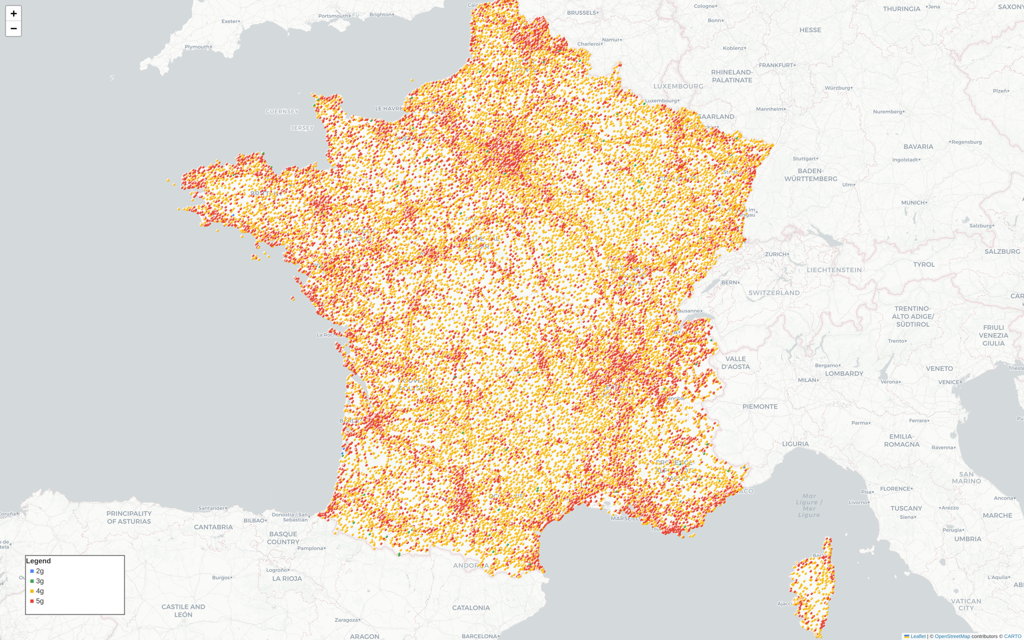
\includegraphics[width=0.7\textwidth]{images/France-Technologies.png}
        \caption{\label{fig:fr-tech}Les technologies dans toute la France}
    \end{figure}
\end{frame}

\begin{frame}{}
    \begin{figure}
        \includegraphics[width=0.7\textwidth]{images/Normandie-Opérateurs.png}
        \caption{\label{fig:no-op}Les opérateurs en Normandie}
    \end{figure}
\end{frame}

\begin{frame}{}
    \begin{figure}
        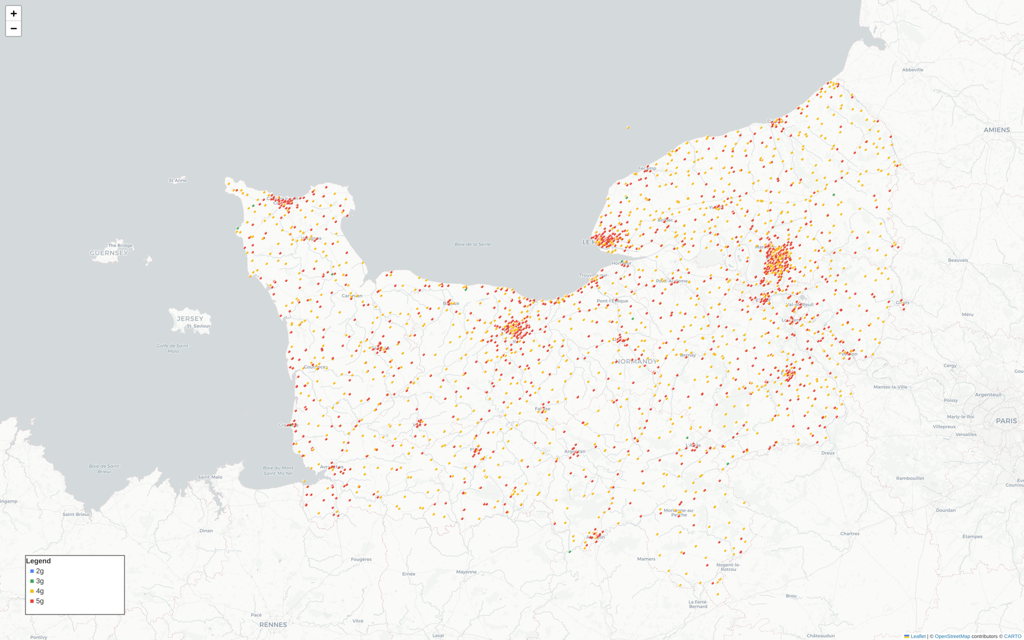
\includegraphics[width=0.7\textwidth]{images/Normandie-Technologies.png}
        \caption{\label{fig:no-tech}Les technologies en Normandie}
    \end{figure}
\end{frame}

\subsubsection{DBScan}
\begin{frame}{Détection des villes}
    Il est très clair que les stations de bases sont très regroupé au sein des villes. Il semble donc qu'il soit possible de détecter si les stations de bases sont en zone rurale ou urbaine à l'aide de la densité de stations de base

    \begin{block}{DBscan (1996)}
        L'algorithme DBscan (Density-Based spatial clustering of applications with noise) est un algorithme qui s'appuie sur la densité estimée des clusters pour effectuer le partitionnement.
    \end{block}
    \begin{block}{Paramètres}
        \begin{itemize}
            \item $\varepsilon$ : dissimilarité maximum entre deux individus ;
            \item $n_{\min}$ : cardinal minimum de chaque classe.
        \end{itemize}
    \end{block}
\end{frame}

\begin{frame}{Théorie : l'algorithme}
    \begin{block}{}
        \begin{enumerate}
            \item Pour chaque point $p_{j}$ :
                \begin{align*}
                    N\left(p_{i}\right) & \gets\left\{ p_{j}, j\in N=\left\{ 1, \dots, n\right\} \mid d(i,j)\leqslant\varepsilon\right\} \\
                    C & \gets\left\{ p_{i}\mid\left|N\left(p_{i}\right)\right|\geqslant n_{\min}\right\} 
                \end{align*}
            \item Construire le graphe de voisinage $G=\left(X, U\right)$, avec $$X=\left\{ p_{i}\mid i\in N\right\} \text{ et } U=\left\{ ij\mid i, j\in N,d(i,j)\leqslant\varepsilon\right\}$$
            \item Trouver les composantes connexes des sommets de $G$ (notées $G_{1}, \dots, G_{p}$) ;
            \item Pour chaque $p_{i}\notin C$ :
                \begin{align*}
                    j^{*} & =\arg\min_{1, \dots, p}\left(d\left(p_{i}, C_{k}\right)\right)\\
                    \text{si } & d\left(p_{i}, C_{j^{*}}\right)\leqslant\varepsilon\text{ alors}\\
                     & C_{j^{*}}\gets C_{j^{*}}\cup\left\{ p_{i}\right\} 
                \end{align*}
        \end{enumerate}
    \end{block}    
\end{frame}

\begin{frame}{}
    \begin{figure}
        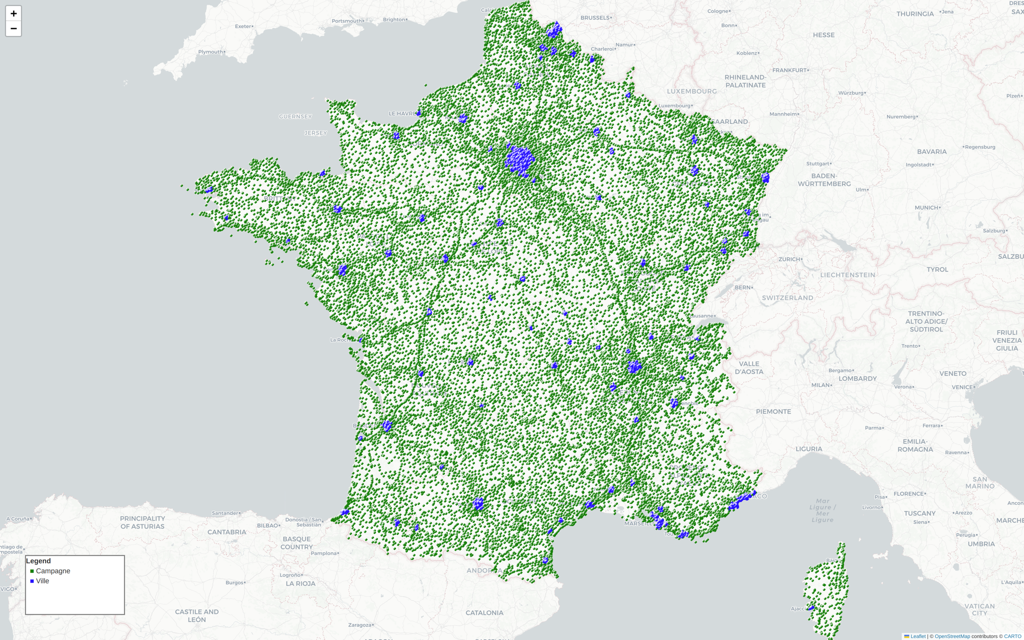
\includegraphics[width=0.7\textwidth]{images/France-Villes-Orange_0.03_15.png}
        \caption{\label{fig:fr-vi-or-0.03-15}Les villes détectées en France pour l'opérateur Orange avec $\epsilon=0.03$ et $n_{min}=15$}
    \end{figure}
\end{frame}


\subsubsection{Delaunay et Voronoï}

\begin{frame}{Diagramme de Voronoï}
    \begin{columns}
        \begin{column}{0.6\textwidth}
            \begin{block}{Définition}
                Le diagramme de Voronoï associé à un ensemble de points $(d_i)_{1\leq i \leq n}$ est un pavage de l'espace tel que chaque pavé $P_i$ représente l'ensemble des points plus proches de $d_i$ que de n'importe quel $d_j$ avec $j\neq i$ i.e.
            \end{block}
        \end{column}
            
        \begin{column}{0.4\textwidth}
            \begin{figure}
                
\includegraphics[width=0.5\textwidth]{images/Coloured_Voronoi_2D.png}
                \caption{\label{fig:vor-ex}Exemple de diagramme de Voronoï}
            \end{figure}
        \end{column}
    \end{columns}
    
            
\end{frame}

\begin{frame}{Triangulation de Delaunay}
    \begin{columns}
        \begin{column}{0.6\textwidth}
            \begin{block}{Définition}
                La triangulation de Delaunay d'un ensemble $P$ de points du plan est une triangulation $DT(P)$ telle qu'aucun point de $P$ n'est à l'intérieur du cercle circonscrit d'un des triangles de $DT(P)$. Les triangulations de Delaunay maximisent le plus petit angle de l'ensemble des angles des triangles, évitant ainsi les triangles \og allongés \fg{}.
            \end{block}
        \end{column}
            
        \begin{column}{0.4\textwidth}
             \begin{figure}
                
\includegraphics[width=0.5\textwidth]{images/Delaunay_circumcircles_vectorial.svg.png}
                \caption{\label{fig:del-ex}Exemple de triangulation de Delaunay}
            \end{figure}
        \end{column}
    \end{columns}
\end{frame}

\begin{frame}{Lien entre les 2}
    \begin{columns}
        \begin{column}{0.6\textwidth}
            \begin{block}{Propriétés}
                \begin{itemize}
                    \item La triangulation de Delaunay d’un ensemble discret $P$ de points est le graphe dual du diagramme de Voronoï associé à $P$;
                    \item Il est donc très facile de passer de l'un à l'autre (en temps polynomial);
                    \item il existe des algorithmes pour trouver une triangulation de Delaunay en $O(n\log(n))$.
                \end{itemize}      
            \end{block} 
        \end{column}
            
        \begin{column}{0.4\textwidth}
            \begin{figure}
                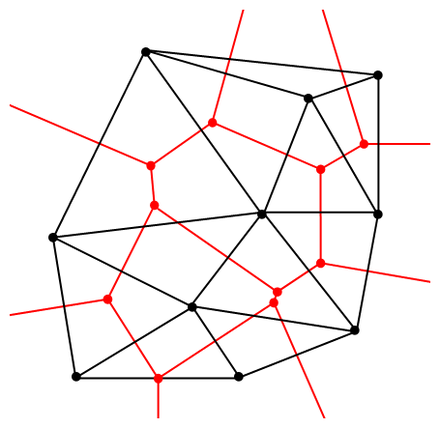
\includegraphics[width=0.5\textwidth]{images/Delaunay_Voronoi.png}
                \caption{\label{fig:del-vor}Lien entre Delaunay et Voronoï}
            \end{figure}
        \end{column}
    \end{columns} 
\end{frame}

\begin{frame}{Retour au problème}
    \begin{block}{Application à notre cas d'étude}
        Nous allons pouvoir utiliser ces notions en définissant :
        \begin{itemize}
            \item les voisins potentiels comme étant les triangles adjacents dans la triangulation de Delaunay
            \item les zones de couverture des antennes comme les pavés associé dans le diagramme de Voronoï
        \end{itemize}
    \end{block}
\end{frame}
}

\subsection{Paul}
\insertsubsectionframe

\begin{frame}{Résumé des épisodes précédents}
    Mon travail, pour la semaine qui vient de s'écouler, s'articule autour de trois axes majeurs :
    \begin{block}{}
        \begin{itemize}
            \item Découverte des données ;
            \item Documentation ;
            \item Reprise du travail de l'année précédente.
        \end{itemize}
    \end{block}
        
\end{frame}

{
\smallframetitle
\begin{frame}{Documentation}
    La majeure partie du travail de la semaine écoulée a consisté à se former aux différents outils de \texttt{Python} afin de pouvoir effectuer sereinement le travail.

    \begin{block}{Outils utilisés}
        \begin{itemize}
            \item \texttt{pandas.DataFrame} : gestion des données ;
            \item \texttt{scipy.spatial.Delaunay} : création de la triangulation de Delaunay ;
            \item \texttt{networkx.Graph} : création de graphes ;
            \item \texttt{matplotlib.pyplot} : affichage des résultats.
        \end{itemize}
    \end{block}
\end{frame}

\begin{frame}{Reprise du travail précédent (1/3)}
    La première tâche consistait à essayer de faire fonctionner le code fourni. Résultat : il ne fonctionne pas\dots
    
    Décision : refaire par moi-même. Cependant, j'ai gardé les idées.
    \begin{block}{Approche pour déterminer les voisins de stations de base}
        \begin{itemize}
            \item Faire une triangulation de Delaunay (liste de voisins potentiels);
            \item Eliminer les voisins distants de plus de $\unit[15]{km}$ ;
            \item Garder le voisin le plus proche dans chaque cadrant autour de chaque station (6 cadrants);
            \item Garder le voisin le plus proche quand deux stations voisines sont séparées par un angle faible.
        \end{itemize}
            
    \end{block}
\end{frame}

\begin{frame}{Reprise du travail précédent (2/3)}
    Ayant refait l'implantation moi-même, j'ai décidé d'utiliser les graphes au lieu de simplement les datasFrames : permettra de faciliter l'application de la théorie des graphes.
    \begin{block}{Apports de cette nouvelle représentation}
        \begin{itemize}
            \item On travail directement sur le graphe de Delaunay ;
            \item Le traitement des voisins est beaucoup plus facile ;
            \item La représentation graphique est plus claire.
        \end{itemize}
    \end{block}
\end{frame}

\begin{frame}{Reprise du travail précédent (3/3) : Résultats}
    Pour l'instant seul les deux premiers critères de filtrage sont fonctionnels. Voici ce que l'on obtient sur le département du Gard :
    \begin{figure}
        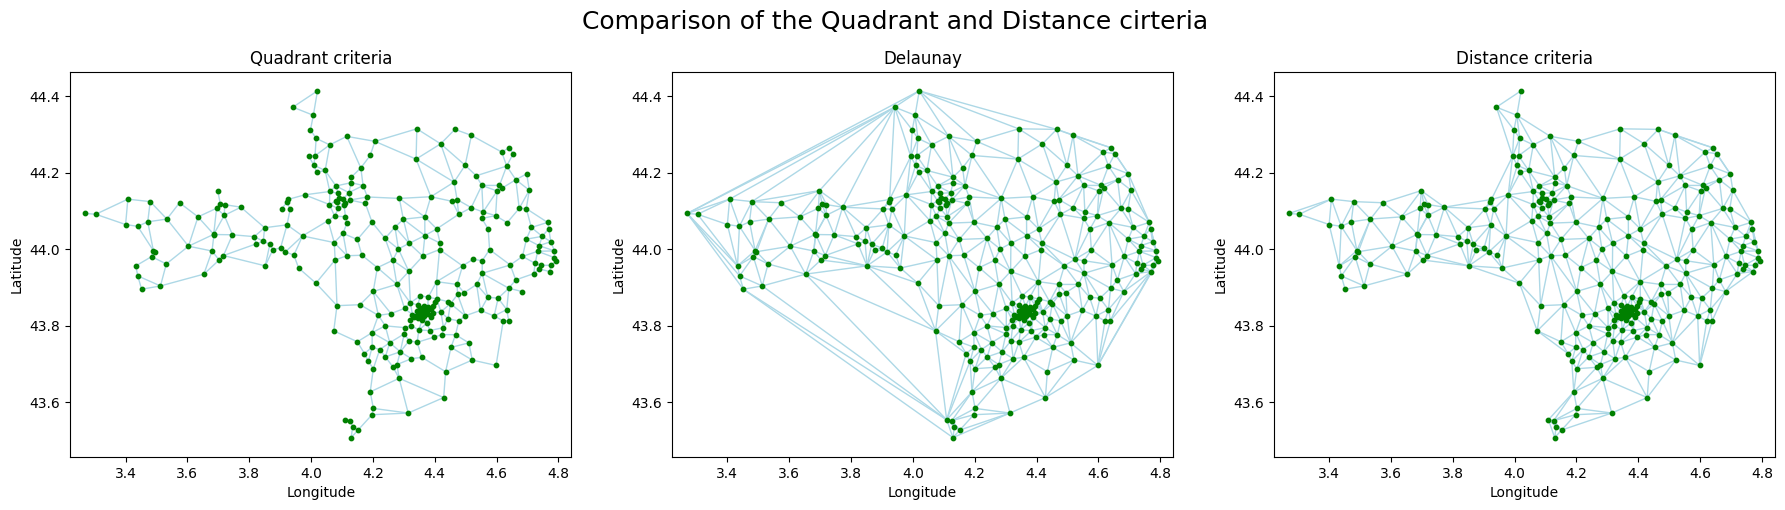
\includegraphics[width=0.9\textwidth]{images/comparaison_criteres.png}
        \caption{\label{fig:comp-crit}Evolution de la triangulation de Delaunay en fonction de critères de filtrage}
    \end{figure}
\end{frame}

\begin{frame}{Perspectives d'amélioration et travail à venir}
    \begin{block}{Améliorations}
        \begin{itemize} 
            \item Vérifier que l'algorithme du critère du quadrant donne les bons résultats;
            \item Optimisation dudit algorithme.
        \end{itemize}
    \end{block}

    \begin{block}{Travail à venir}
        \begin{itemize} 
            \item Implanter une version fonctionnelle du critère de l'angle;
            \item Se renseigner sur l'état de l'art de la théorie des graphes.
        \end{itemize}
    \end{block}
\end{frame}
}




\subsection{Brendan}
\insertsubsectionframe
\begin{frame}{Réalisation d'une interface graphique en \texttt{Python}}
    \begin{block}{Contexte}
        \begin{itemize}
            \item Beaucoup de cartes à tracer car beaucoup de paramètres ;
            \item Cartes gourmandes en ressources et pas adaptées à des notebooks \texttt{Python} ;
            \item Réalisation d'une application permettant de facilement tracer ces cartes au sein d'un navigateur web.
        \end{itemize}
    \end{block}
    
\end{frame}

% \smallframetitle

\section{Semaine du 14/05/24 au 21/05/24}
\insertsectionframe
\subsection{Le jeu de donnée}
\insertsubsectionframe

\begin{frame}{Le jeu de donnée}
    \begin{block}{Arcep}
        L'autorité de régulation des communications électroniques, des postes et de la distribution de la presse (Arcep) est une autorité administrative indépendante française chargée de réguler les communications électroniques et postales et la distribution de la presse.
    \end{block}

    \begin{block}{Mon Réseau Mobile}
        Mon Réseau Mobile est la plate-forme cartographique regroupant l’ensemble des données géographiques en lien avec les réseaux dits \og mobiles \fg{} (2G, 3G, 4G, 5G) régulés par l’Arcep.
    \end{block}

    \begin{alertblock}{Nouvelle mise à jour}
        Une nouvelle mise à jour des données est prévue de \textbf{jeudi 20 juin 2024} à 17h40 : données du 1\ier{} trimestre de 2024.
    \end{alertblock}

    A cette adresse : \url{https://www.data.gouv.fr/fr/datasets/mon-reseau-mobile/\#/discussions}, on peut poser nos questions sur le jeu de données.
\end{frame}


\begin{frame}{Arborescence du jeu de données}
    \begin{columns}
        \begin{column}{0.4\textwidth}
            Les fichiers de données sont rangés par trimestre de publication, zone (France métropolitaine/Outre-mer) et département le cas échéant :
        \end{column}
            
        \begin{column}{0.6\textwidth}
            \begin{figure}
                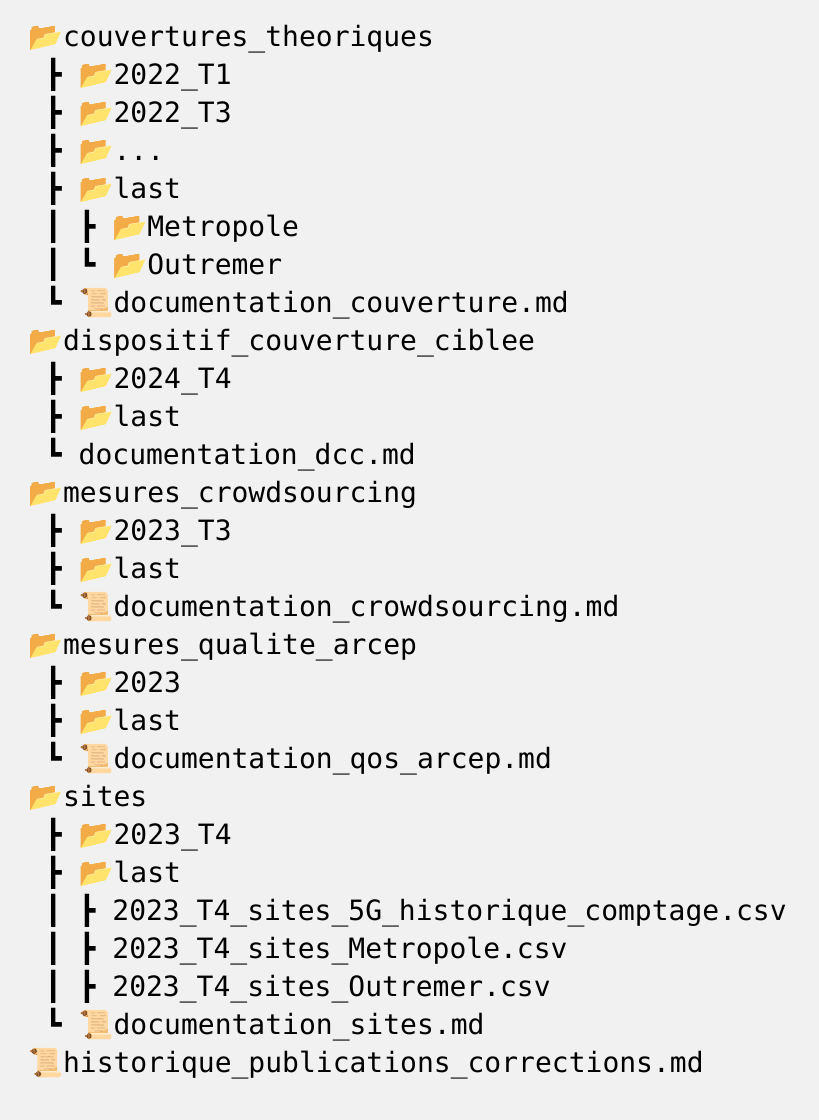
\includegraphics[height=0.55\paperheight]{images/architecture.png}
                \caption{\label{fig:archi}Architecture de la base de donnée}
            \end{figure}
        \end{column}
    \end{columns} 
    
\end{frame}

\begin{frame}{Fréquences de mises à jour}
    \begin{figure}
        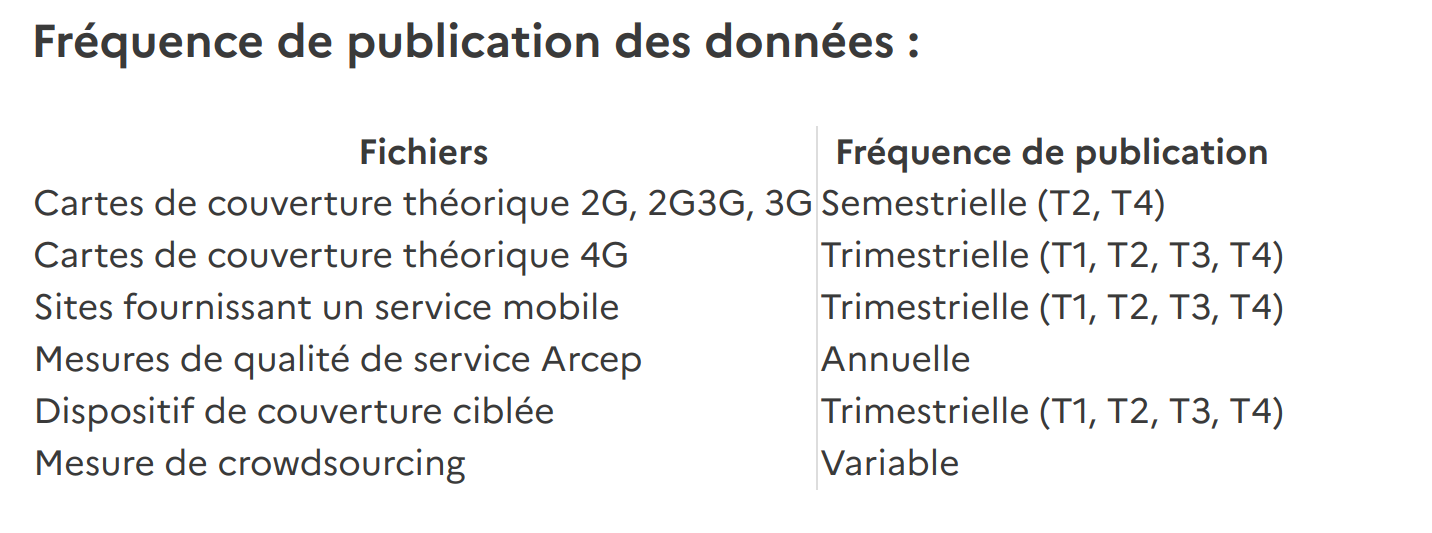
\includegraphics[height=0.5\paperheight]{images/frequence.png}
        \caption{\label{fig:freq}Fréquence de publication de mises à jour}
    \end{figure}
\end{frame}


\subsection{Faisons parler les données}
\insertsubsectionframe

\begin{frame}{Quelques chiffres en vrac}
    Tout d'abord, remarquons que chaque station peut être identifiée à son \texttt{num\_site} (seul deux stations n'en n'ont pas).
    Ensuite, voici ce que l'on a découvert :
    \begin{block}{Des chiffres sympathiques}
        \begin{itemize}
            \item \texttt{site\_zb} : $10\,596$ (Site issu du programme \og zones blanches – centres-bourgs\fg{}) ;
            \item \texttt{site\_dcc} : $10\,627$ (Site issu du \og Dispositif de Couverture Ciblée\fg{}) ;
            \item \texttt{site\_strategique} : $144$ (Site issu du programme \og France Mobile\fg{}) ;
            \item \texttt{mes\_4g\_trim} : $1\,618$ (Equipement du site en technologie 4g au cours du dernier trimestre (du 30/06/2022 au 30/09/2022)) ;
            \item \texttt{id\_site\_partage} : $5\,453$ (Sites mutualisés entre plusieurs opérateurs) ;
            \item \texttt{site\_capa\_204mbps} : $92\,664$ (Site dont la capacité maximum théorique est supérieure ou égale à $\unit[240]{Mbs}$).
        \end{itemize}
    \end{block}
\end{frame}

\begin{frame}{Quelques chiffres en vrac : précision sur les indicateurs}
    Ensuite, voici ce que l'on a découvert :
    \begin{block}{\texttt{site\_zb}}
        Le premier programme, initié en 2003 et nommé \og zones blanches – centres-bourgs\fg{} consistait à apporter des services de téléphonie mobile, SMS et internet mobile à très haut débit, dans plus de 3500 centres-bourgs de communes de France qui ne bénéficiaient d’aucune couverture mobile.
        \footnotemark[1]
    \end{block}

    \begin{block}{\texttt{site\_dcc}}
        Le dispositif de couverture ciblée vise à assurer une couverture mobile de qualité dans des zones non ou mal couvertes, en construisant jusqu’à 5 000 nouveaux sites par opérateur, dont une partie sera mutualisée.
        \footnotemark[2]
    \end{block}
    
    \footnotetext[1]{\url{https://www.tactis.fr/zone-blanche-zone-grise/}}
    \footnotetext[2]{\url{https://agence-cohesion-territoires.gouv.fr/france-mobile-54}}
\end{frame}



\begin{frame}{Comparaison des différents équipements en terme de technologies (1/7)}
    Voici tout d'abord un graphique sur la présence d'une technologie en fonction de l'opérateur (une technologie présente sur un site n'exclue pas la présence d'une autre technologie) :
    \begin{figure}
        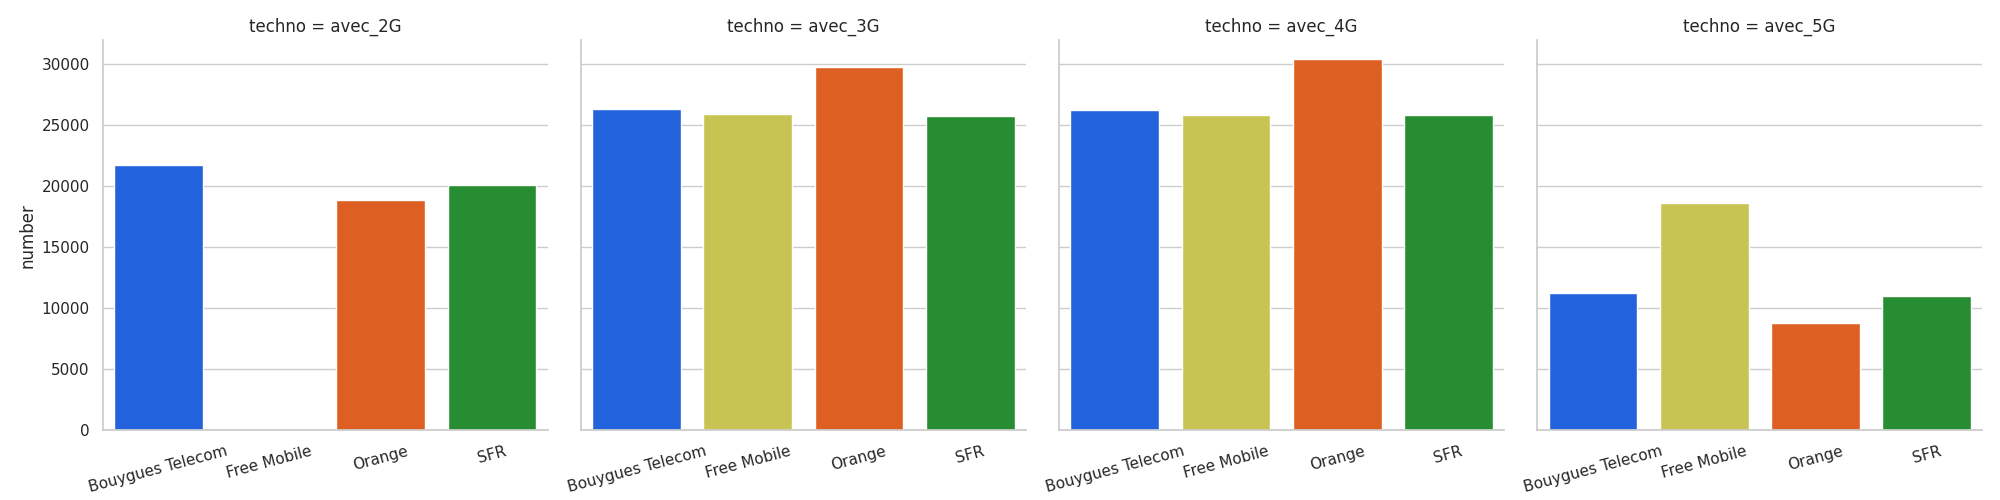
\includegraphics[height=0.4\paperheight]{images/barplots/avec_techno.png}
        \caption{\label{fig:av_tech}Nombres de sites équipés d'au moins une technologie}
    \end{figure}
\end{frame}

\begin{frame}{Comparaison des différents équipements en terme de technologies (2/7)}
    \begin{table}[!ht]
        \centering
        \footnotesize
        \begin{tabular}{cccccc}
        \hline
            \textbf{Technologie} & \textbf{Bouygues Telecom} & \textbf{Free Mobile} & \textbf{Orange} & \textbf{SFR} & \textbf{Total} \\ \hline
            \textbf{2G} & 4 & 0 & 10 & 20 & 34 \\ 
            \textbf{3G} & 30 & 102 & 65 & 37 & 234 \\ 
            \textbf{4G} & 15 & 15 & 602 & 106 & 738 \\ 
            \textbf{5G} & 0 & 0 & 3 & 0 & 3 \\ 
            \textbf{2-3G} & 66 & 0 & 21 & 80 & 167 \\ 
            \textbf{2-4G} & 12 & 0 & 63 & 67 & 142 \\ 
            \textbf{2-5G} & 0 & 0 & 0 & 0 & 0 \\ 
            \textbf{3-4G} & 3889 & 7225 & 9288 & 4909 & 25311 \\ 
            \textbf{3-5G} & 0 & 0 & 0 & 0 & 0 \\ 
            \textbf{4-5G} & 6 & 0 & 109 & 38 & 153 \\ 
            \textbf{2-3-4G} & 11044 & 0 & 11697 & 9831 & 32572 \\ 
            \textbf{2-3-5G} & 0 & 0 & 1 & 0 & 1 \\ 
            \textbf{2-4-5G} & 0 & 0 & 5 & 10 & 15 \\ 
            \textbf{3-4-5G} & 681 & 18607 & 1638 & 835 & 21761 \\ 
            \textbf{2-3-4-5G} & 10584 & 0 & 7038 & 10085 & 27707 \\ 
            \textbf{Total} & 26331 & 25949 & 30540 & 26018 & 108838 \\ \hline
        \end{tabular}
        \caption{Résumé des données de présence de technologie}
    \end{table}
\end{frame}

\begin{frame}{Comparaison des différents équipements en terme de technologies (3/7)}
    Maintenant nous nous intéressons à la fréquence de présence de certaines technologies et pas d'autres :
    \begin{figure}
        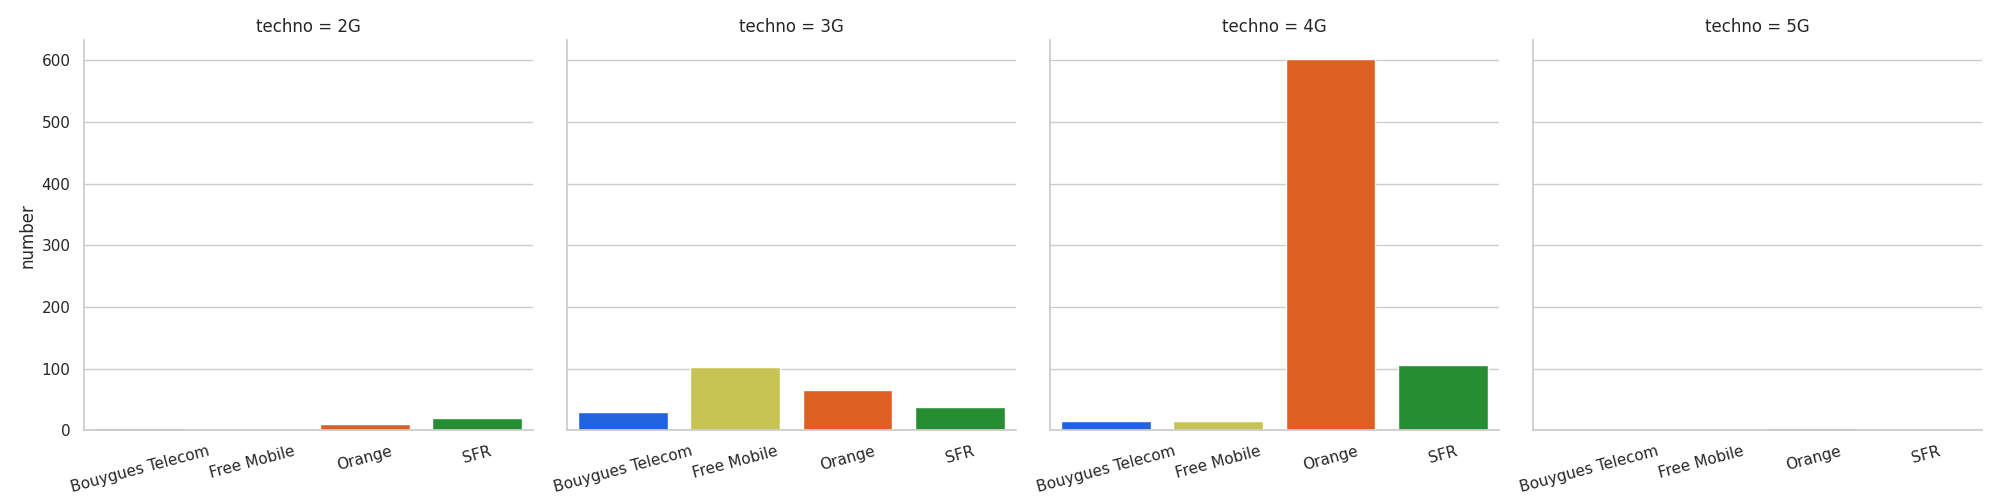
\includegraphics[height=0.4\paperheight]{images/barplots/xG.png}
        \caption{\label{fig:xG}Nombres de sites équipés d'une unique technologie}
    \end{figure}
\end{frame}

\begin{frame}{Comparaison des différents équipements en terme de technologies (4/7)}
    \begin{figure}
        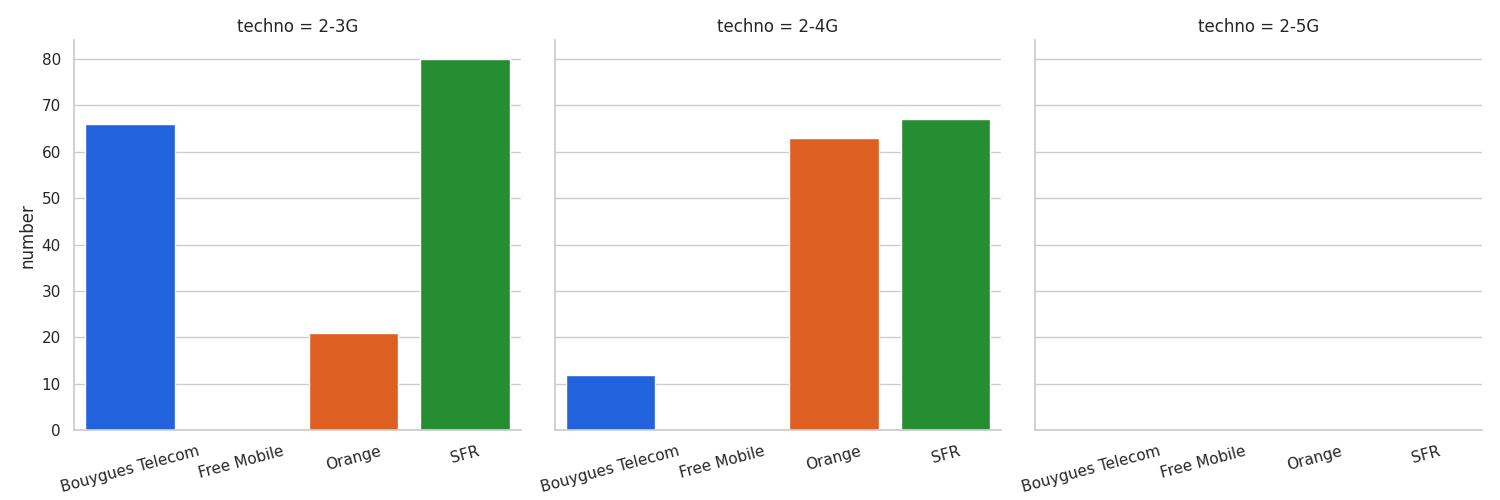
\includegraphics[height=0.4\paperheight]{images/barplots/2-xG.png}
        \caption{\label{fig:2-xG}Nombres de sites équipés de deux technologies}
    \end{figure}
\end{frame}

\begin{frame}{Comparaison des différents équipements en terme de technologies (5/7)}
    \begin{columns}
        \begin{column}{0.65\textwidth}
            \begin{figure}
                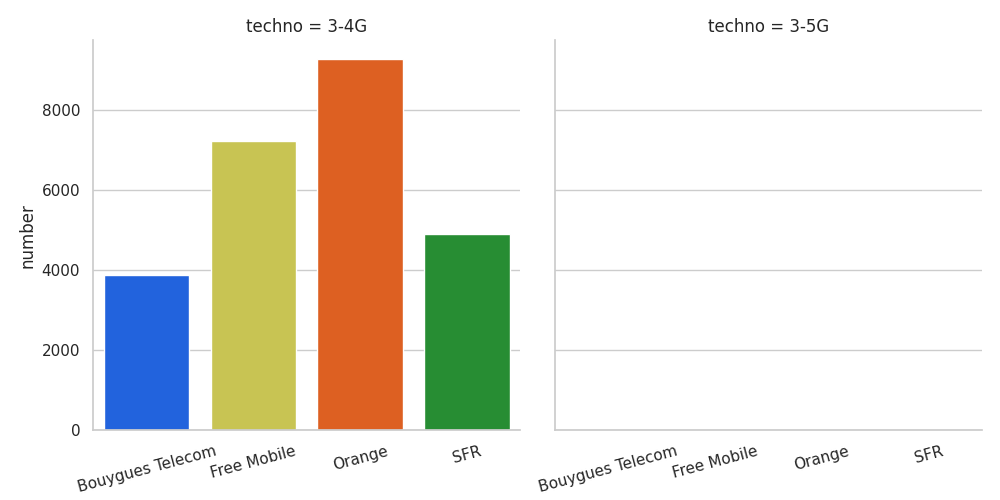
\includegraphics[height=0.4\paperheight]{images/barplots/3-xG.png}
                \caption{\label{fig:3-xG}Nombres de sites équipés de deux technologies (suite)}
            \end{figure}
        \end{column}
            
        \begin{column}{0.35\textwidth}
            \begin{figure}
                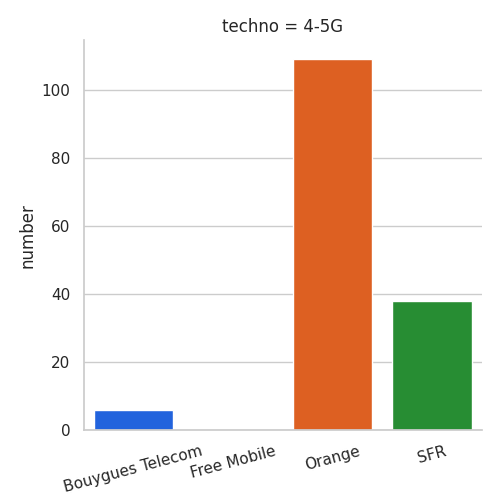
\includegraphics[height=0.4\paperheight]{images/barplots/4-5G.png}
                \caption{\label{fig:4-5G}Nombres de sites équipés de deux technologies (suite-bis)}
            \end{figure}
        \end{column}
    \end{columns} 
\end{frame}

\begin{frame}{Comparaison des différents équipements en terme de technologies (6/7)}
    \begin{figure}
        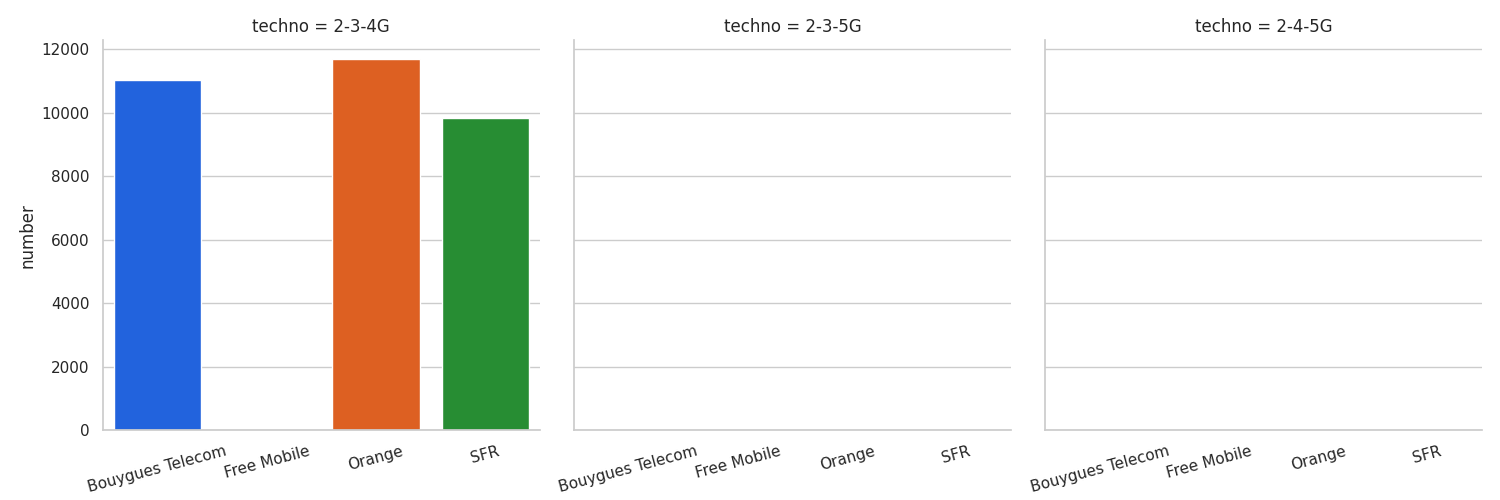
\includegraphics[height=0.4\paperheight]{images/barplots/2-x-yG.png}
        \caption{\label{fig:2-x-yG}Nombres de sites équipés de trois technologies}
    \end{figure}
\end{frame}

\begin{frame}{Comparaison des différents équipements en terme de technologies (7/7)}
    \begin{columns}
        \begin{column}{0.35\textwidth}
            \begin{figure}
                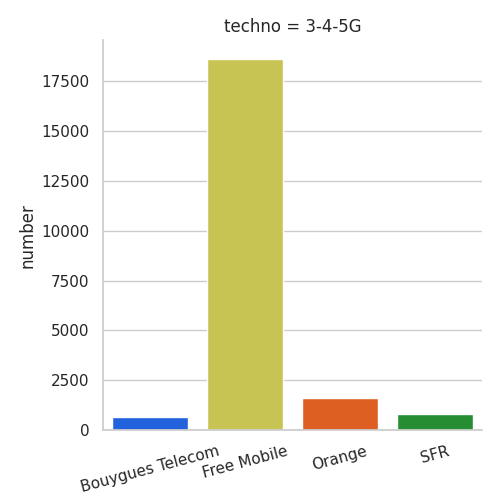
\includegraphics[height=0.4\paperheight]{images/barplots/3-4-5G.png}
                \caption{\label{fig:3-4-5G}Nombres de sites équipés de trois technologies (suite)}
            \end{figure}
        \end{column}
            
        \begin{column}{0.65\textwidth}
            \begin{figure}
                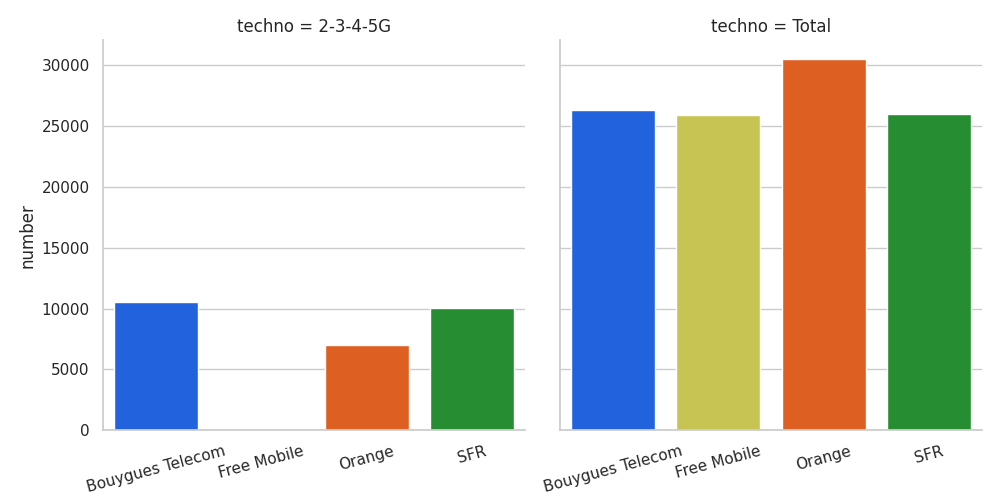
\includegraphics[height=0.4\paperheight]{images/barplots/all-tot.png}
                \caption{\label{fig:all-tot}Nombre de sites équipés de toutes les technologies et total}
            \end{figure}
        \end{column}
    \end{columns} 
\end{frame}

\subsection{Affichage plus détaillé des cartes}
\insertsubsectionframe

\subsubsection{Les stations de base par opérateurs}
\begin{frame}{Les stations de base par opérateur}
    \begin{figure}
        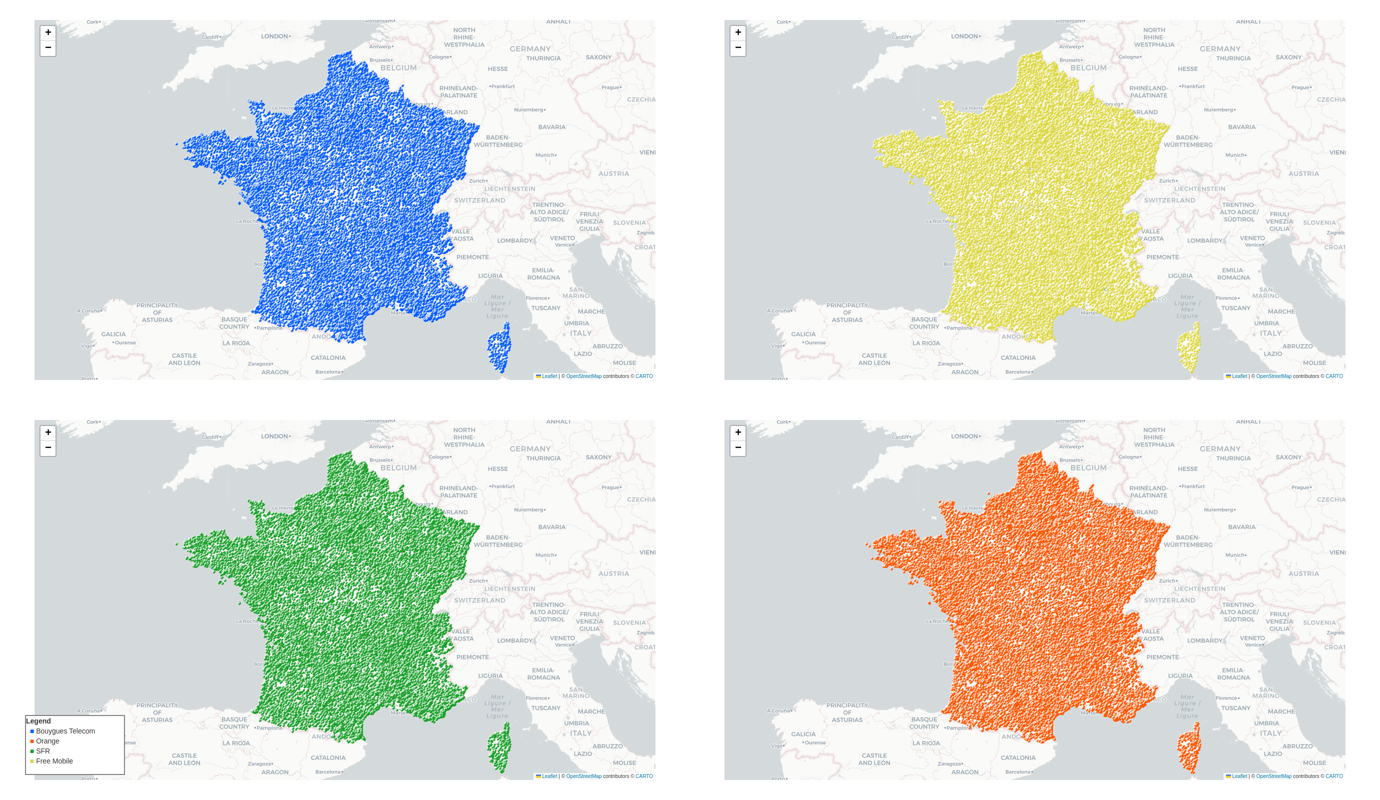
\includegraphics[width=0.9\paperheight]{images/cartes/subplots-providers.png}
        \caption{\label{fig:sp-prov}Les stations de base par opérateurs}
    \end{figure}
\end{frame}


\subsubsection{Les technologies par opérateurs}
\subsubsection{Les technologies par opérateurs}
\begin{frame}{Les stations 2G}
    \begin{figure}
        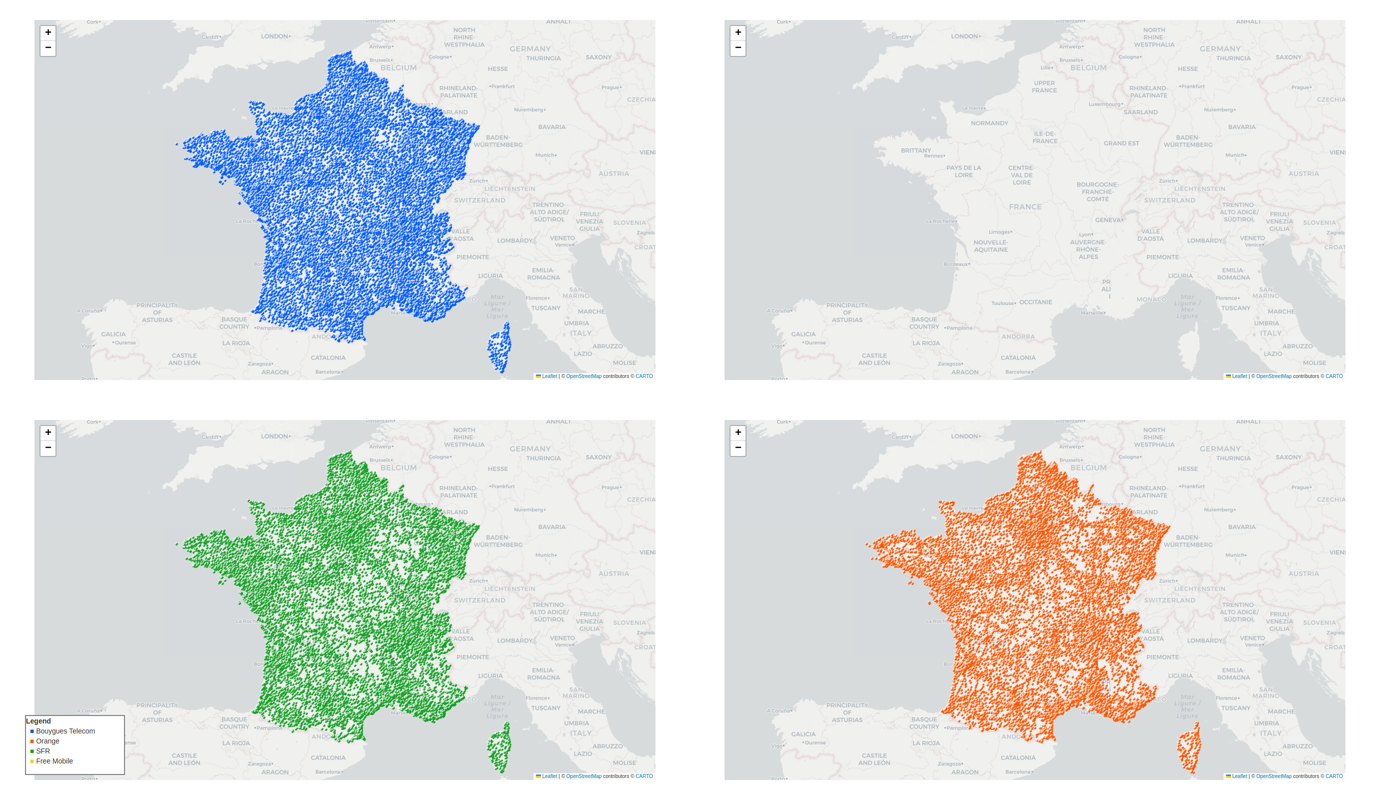
\includegraphics[width=0.9\paperheight]{images/cartes/providers-site_2g.png}
        \caption{\label{fig:sp-2g}Les stations 2G}
    \end{figure}
\end{frame}

\begin{frame}{Les stations 3G}
    \begin{figure}
        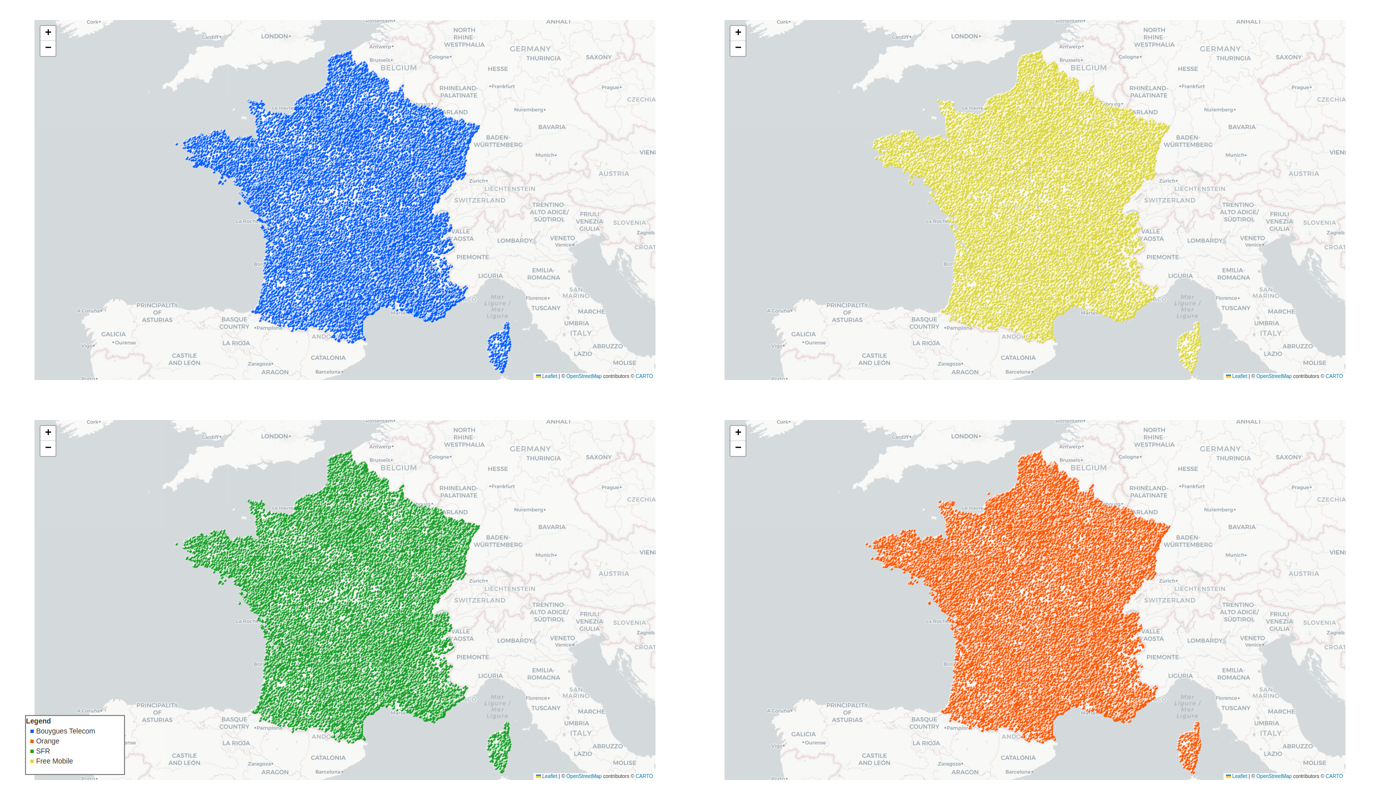
\includegraphics[width=0.9\paperheight]{images/cartes/providers-site_3g.png}
        \caption{\label{fig:sp-3g}Les stations 3G}
    \end{figure}
\end{frame}

\begin{frame}{Les stations 4G}
    \begin{figure}
        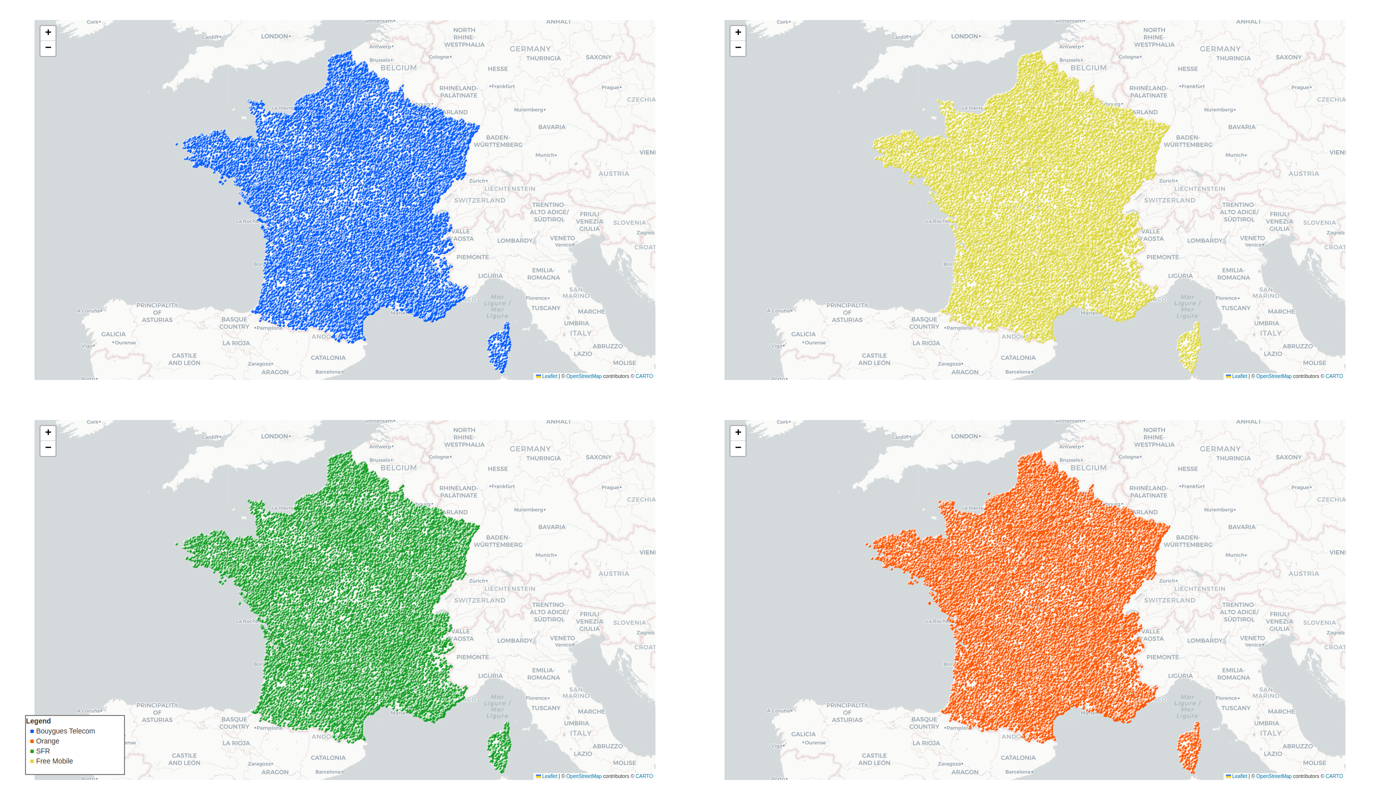
\includegraphics[width=0.9\paperheight]{images/cartes/providers-site_4g.png}
        \caption{\label{fig:sp-4g}Les stations 4G}
    \end{figure}
\end{frame}

\begin{frame}{Les stations 5G}
    \begin{figure}
        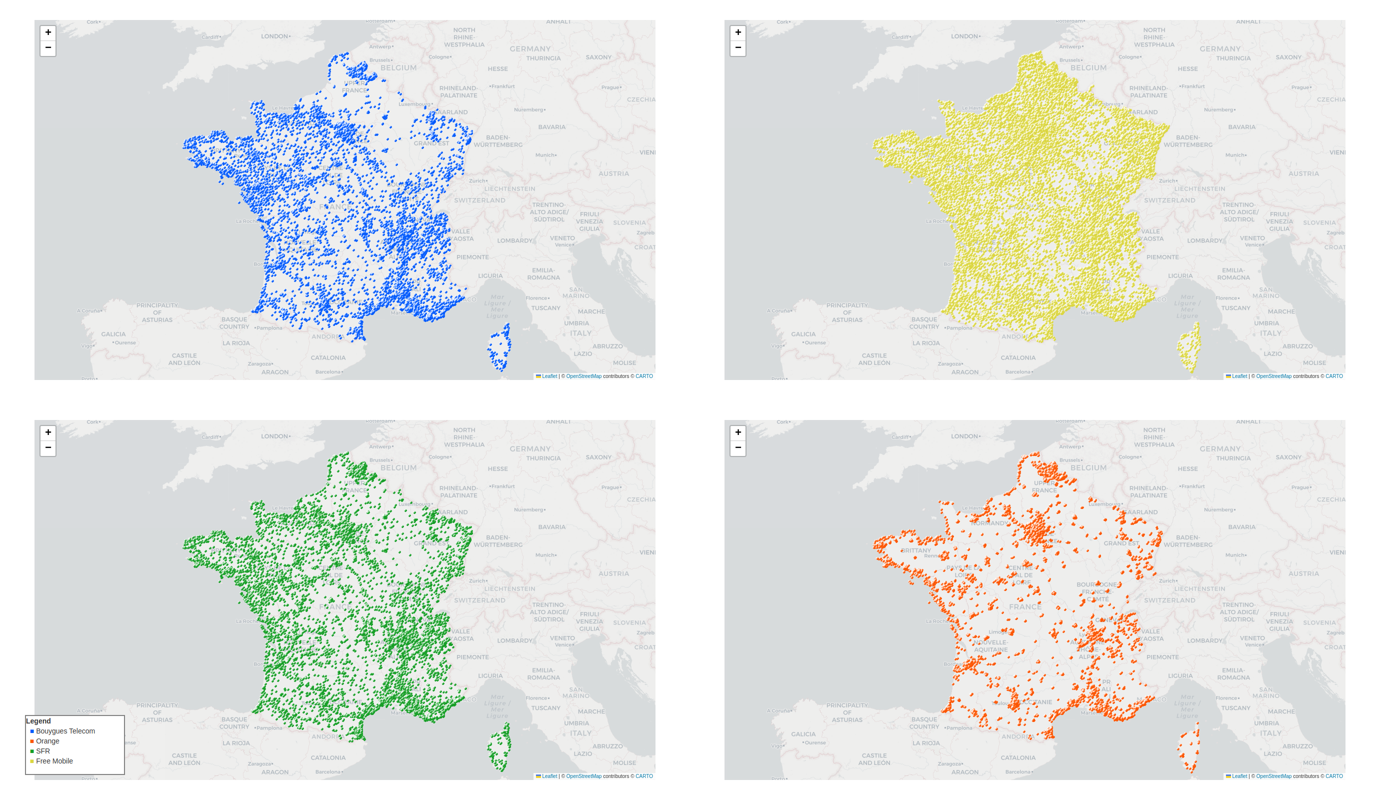
\includegraphics[width=0.9\paperheight]{images/cartes/providers-site_5g.png}
        \caption{\label{fig:sp-5g}Les stations 5G}
    \end{figure}
\end{frame}


\subsection{Evolution du nombre de stations de base au cours du temps}
\insertsubsectionframe

\begin{frame}{2023\_T4\_sites\_5G\_historique\_comptage}
    \begin{figure}
        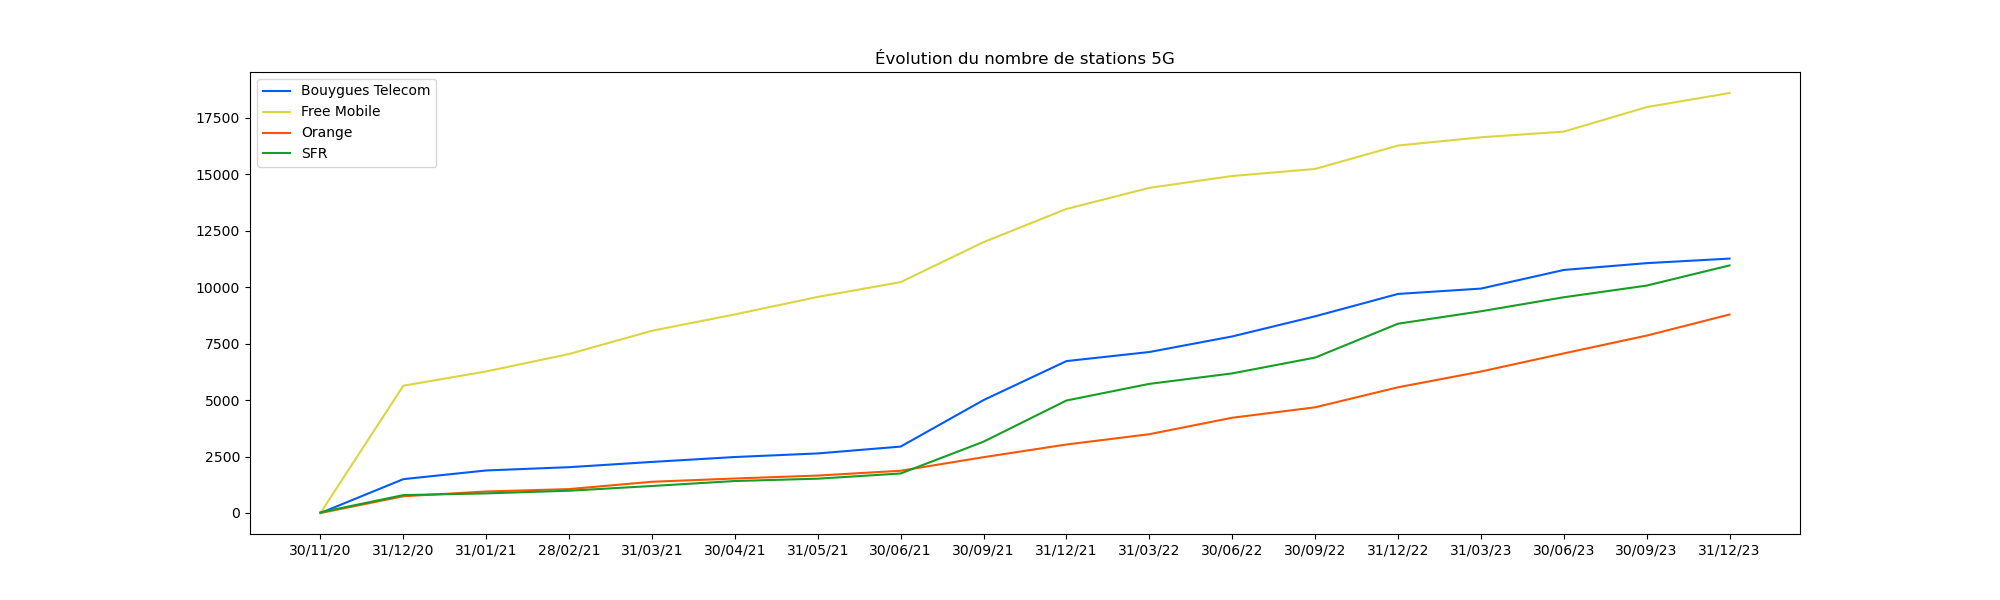
\includegraphics[height=0.5\paperheight]{images/5G-evolution.png}
        \caption{\label{fig:5G-ev}Evolution du nombre de stations 5G en France}
    \end{figure}
\end{frame}


\begin{frame}{Compilation des jeux de données sites}
    \begin{figure}
        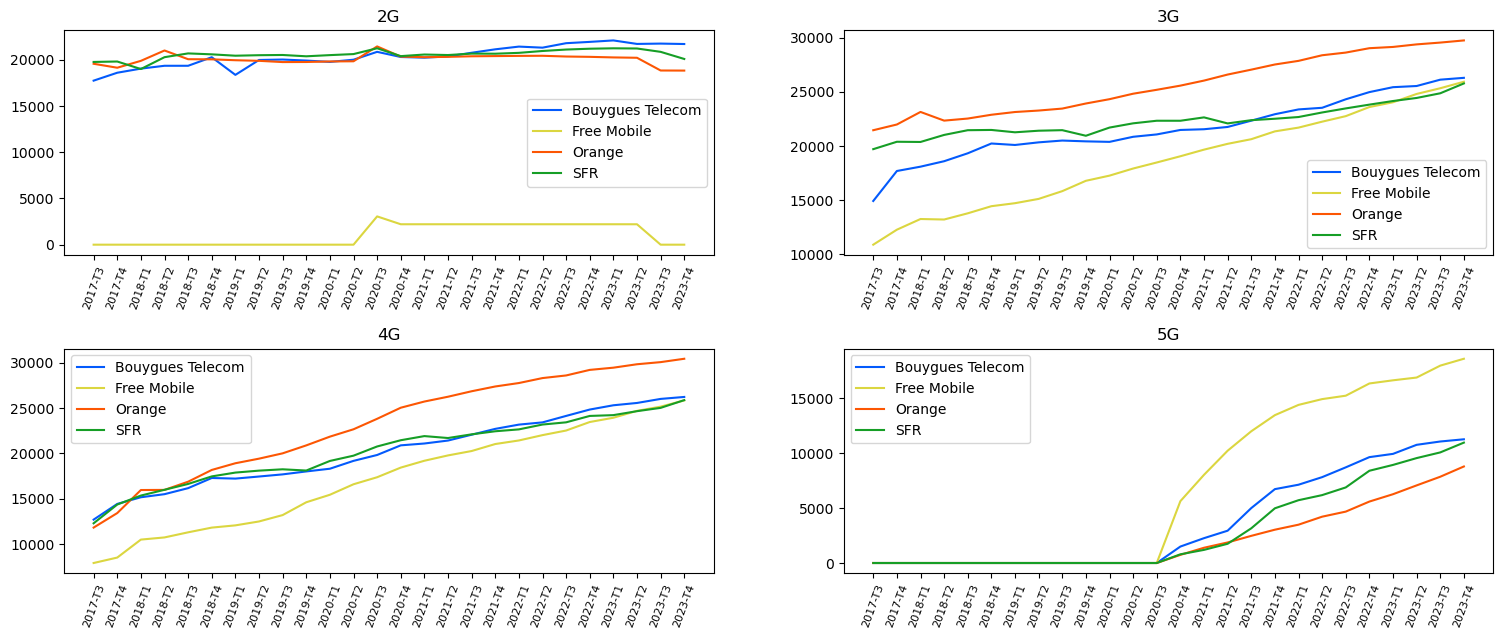
\includegraphics[width=0.78\paperwidth]{images/technos-evolution.png}
        \caption{\label{fig:techno-ev} Evolution du nombre de stations toutes technologies en France}
    \end{figure}
\end{frame}

\begin{frame}{Dispositif de couverture ciblée, éléments d'analyse}
    \begin{block}{infos générales}
        \begin{itemize}
            \item 4621 stations de bases potentielles;
            \item 26 attributs.
        \end{itemize}
    \end{block}

    \begin{block}{anomalies}
        \begin{itemize}
            \item 412 lignes de ce jeu de données ont les colonnes \textbf{x\_lambert\_93} ou \textbf{y\_lambert\_93} non renseigné;
            \item Plusieurs points sont placés en dehors de la France.
        \end{itemize}
    \end{block}
\end{frame}


\begin{frame}{Dispositif de couverture ciblée}
    \begin{figure}
        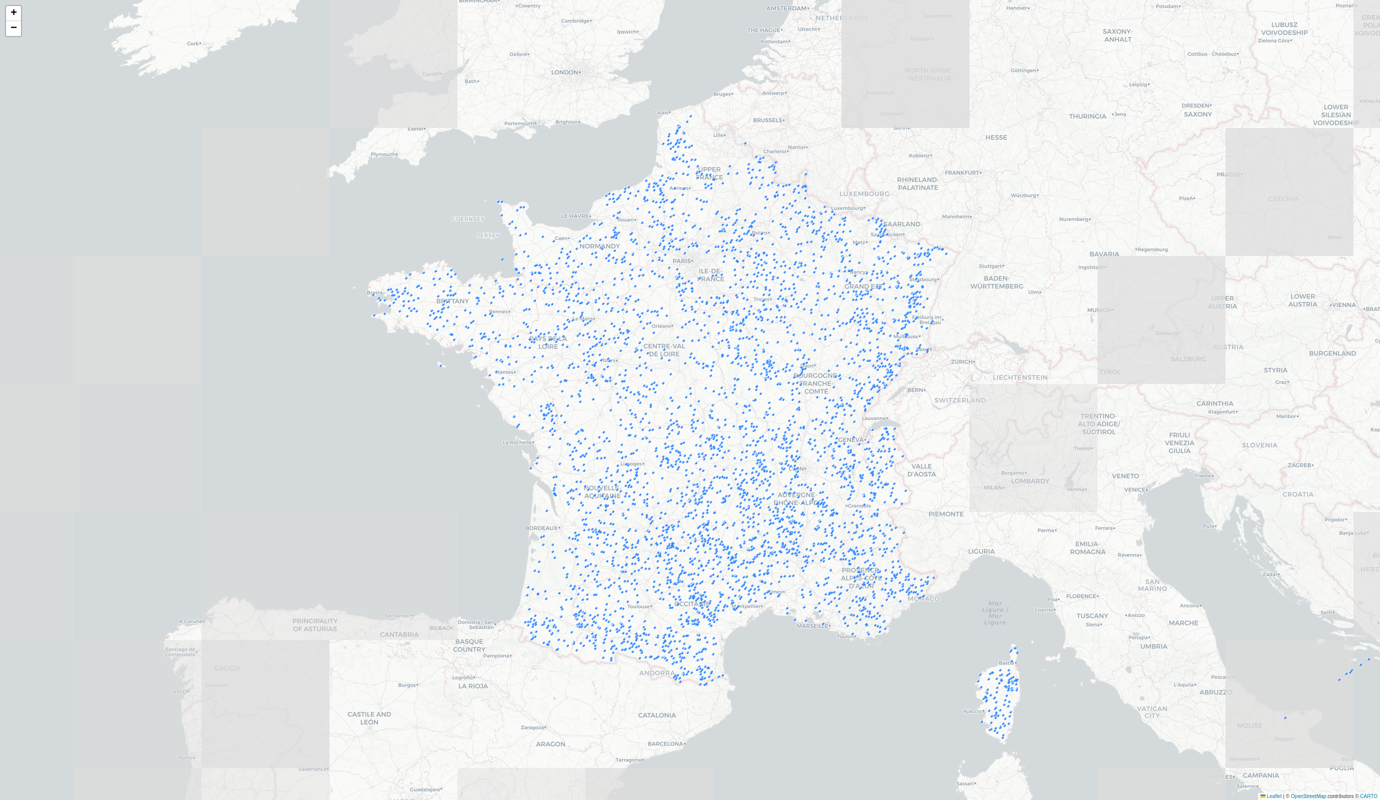
\includegraphics[height=.8\textheight]{images/couverture_ciblee.png}
    \end{figure}
\end{frame}

\begin{frame}{Couverture théorique}
    \begin{block}{Informations}
        \begin{itemize}
            \item format \texttt{.gpkg} (geopackage);
            \item ouverture à l'aide du logiciel libre QGIS.
        \end{itemize}
    \end{block}

    \begin{block}{Utilité}
        \begin{itemize}
            \item Aurait pu permettre de déterminer si 2 stations de base sont voisines (si leur couverture se chevauche);
            \item Non réalisable à l'aide de ce jeu de donnée : seule la couverture globale de chaque région est donnée.
        \end{itemize}
    \end{block}
\end{frame}

\begin{frame}{}
    \begin{figure}
        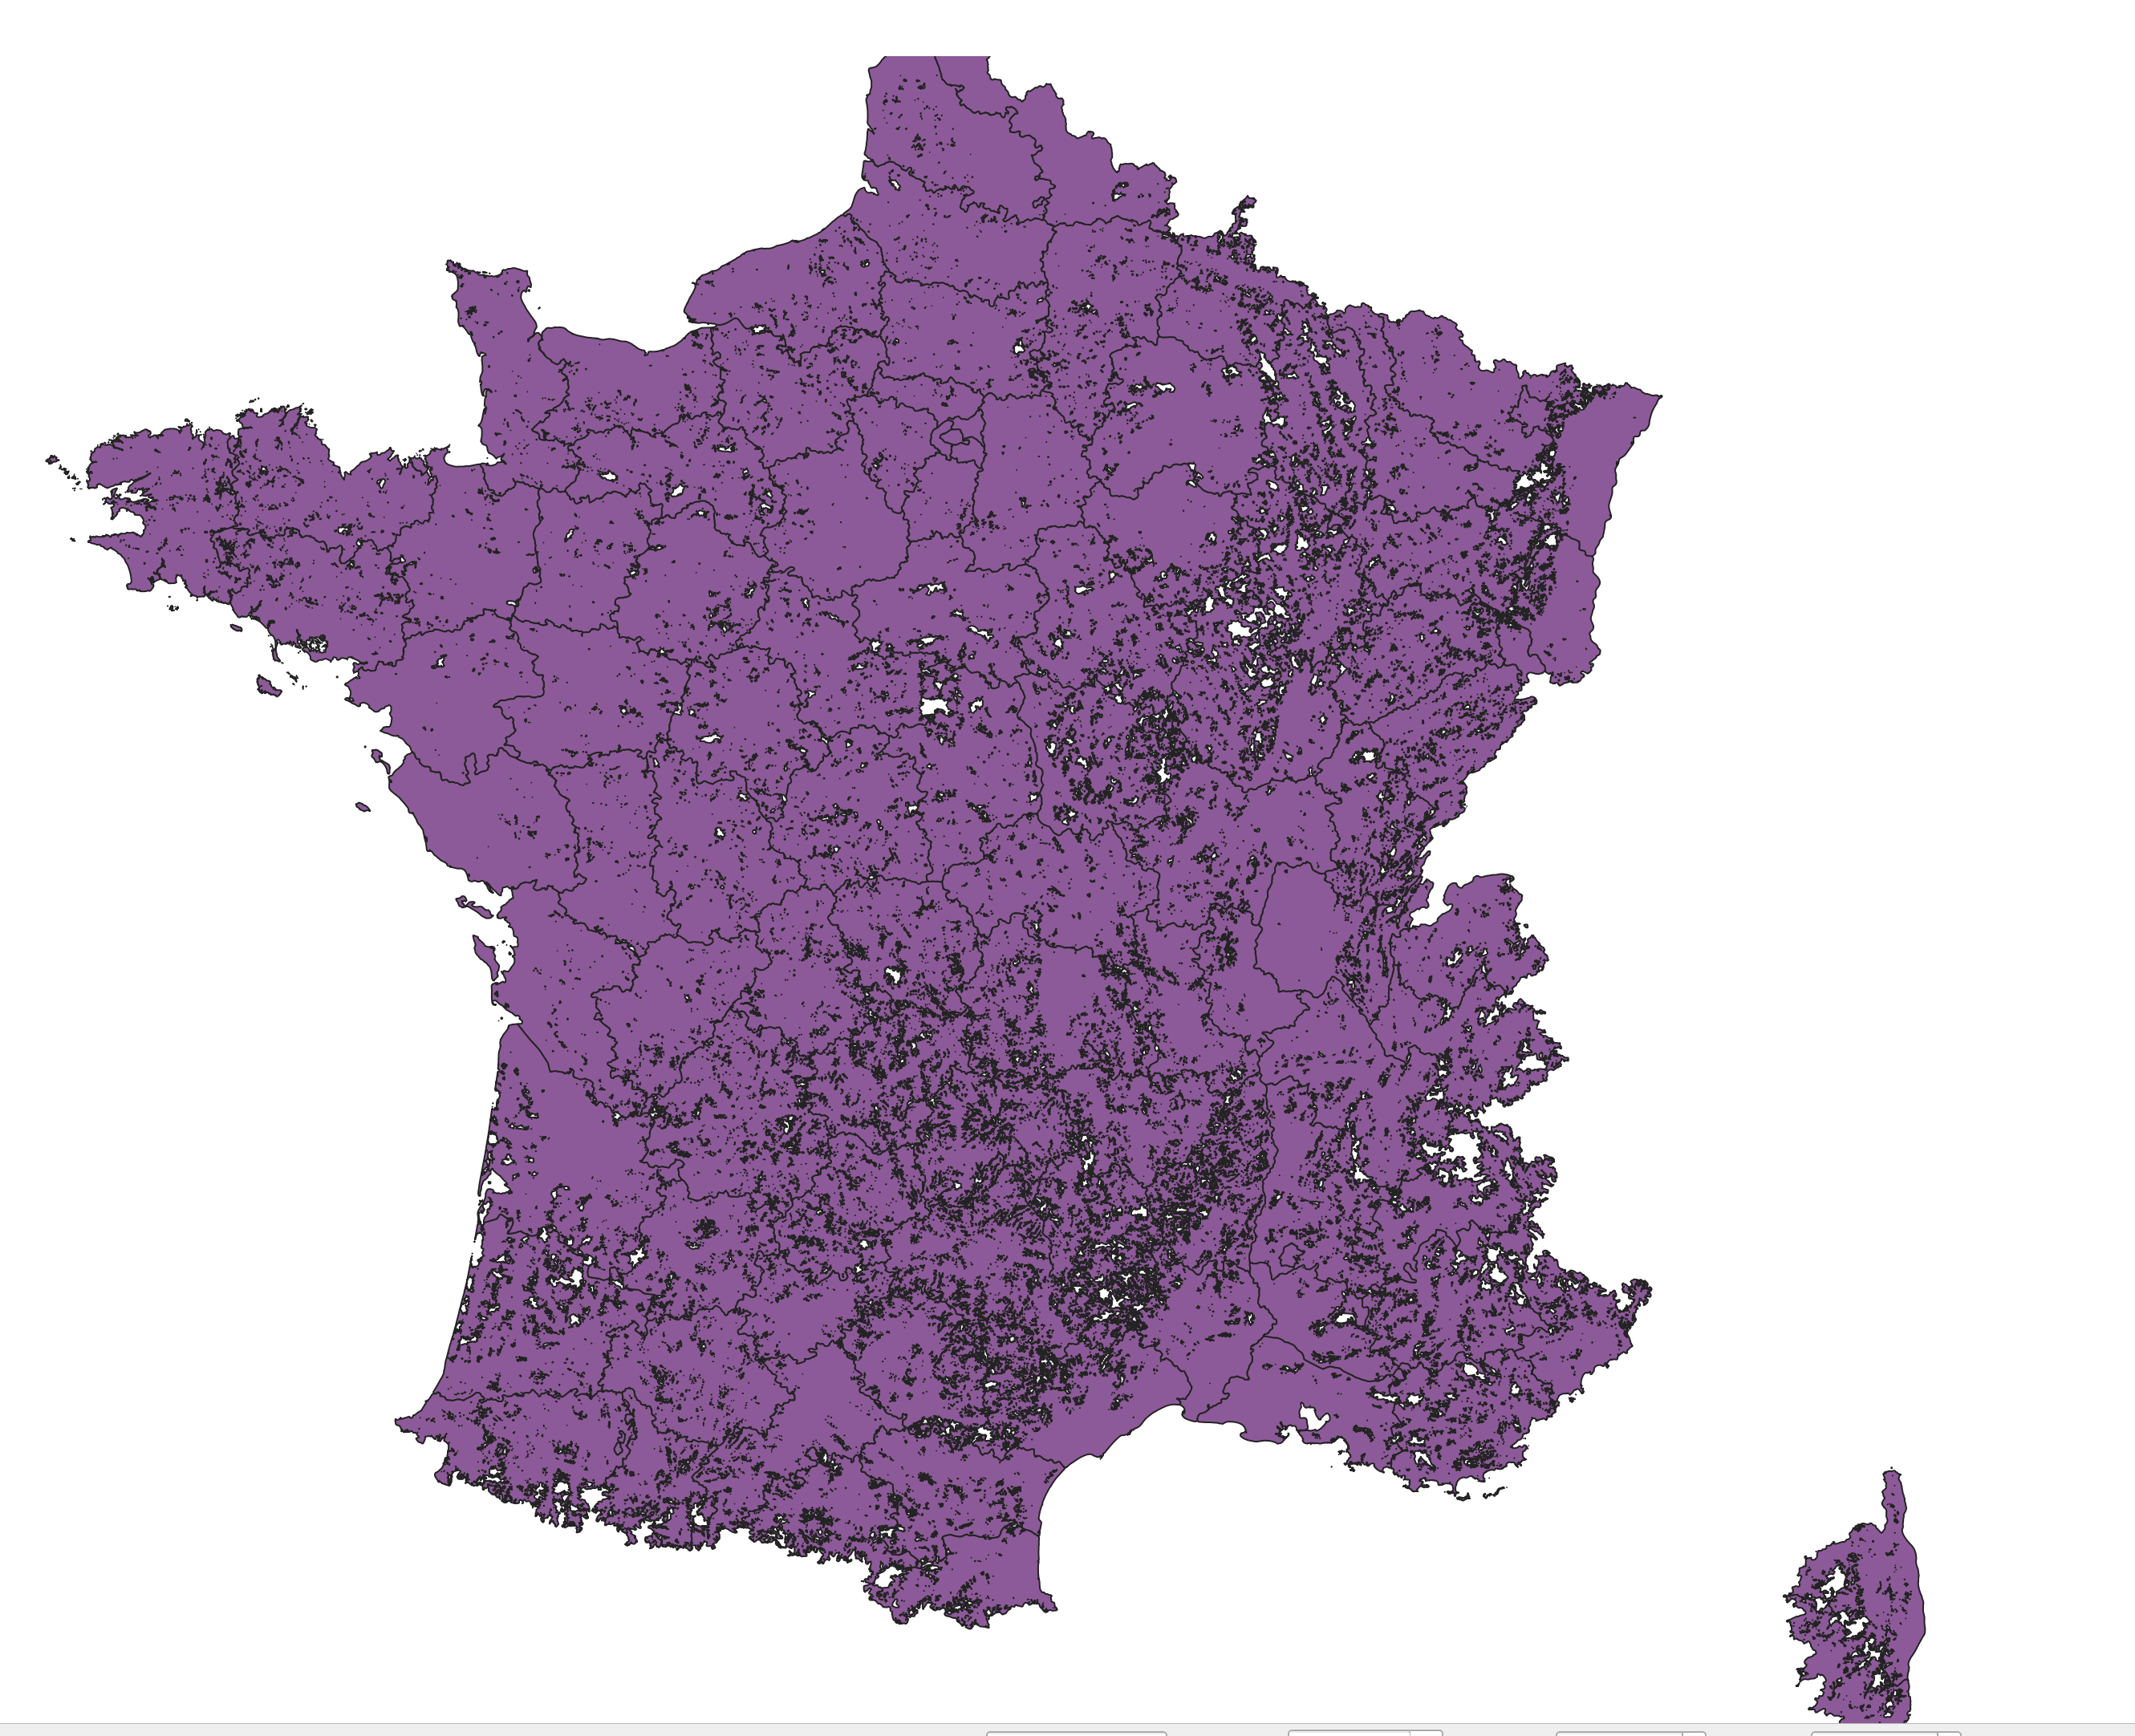
\includegraphics[height=.8\textheight]{images/couverture_theorique_bouygues.png}
    \end{figure}
\end{frame}

% \smallframetitle

\section{Semaine du 21/05/24 au 27/05/24}
\insertsectionframe

\subsection{Statistiques stations de bases - départements}
\insertsubsectionframe

\begin{frame}{Méthodologie}
    On va utiliser une base de donnée complémentaire, reprise de celle trouvée l'année dernière.

    \begin{block}{Une nouvelle base de donnée\footnotemark[1]}
        Cette base de donnée renseigne, par département, la \textbf{superficie} (en $\unit{km^2}$), la \textbf{population} et la \textbf{densité de population} au $\unit{km^2}$.
    \end{block}
    
    A partir de cette base, on va donc pouvoir extraire le nombre d'habitants par stations (normalisé par la taille du département) et la densité de station par département.

    \begin{block}{Calcul du nombre d'habitants par stations normalisé}
        Soit $\lambda$ le nombre d'habitants par stations, par $\unit{km^2}$. Tout d'abord, on se donne $\gamma$, le rapport entre le nombre d'habitant et la surface du département, qui est donné par la densité de population.
        Ensuite, on calcule notre résultat comme suit :$$\lambda = \gamma\times\frac{1}{\text{nombre de stations du département}}$$
    \end{block}

    \footnotetext[1]{\url{https://france.ousuisje.com/departements/classement/superficie.php}}
\end{frame}

\begin{frame}{Nombre d'habitants par stations non normalisé}
    C'est le même calcul que précédemment, sauf qu'à la place de $\gamma$, on utilise simplement la population du département.
    \begin{figure}
        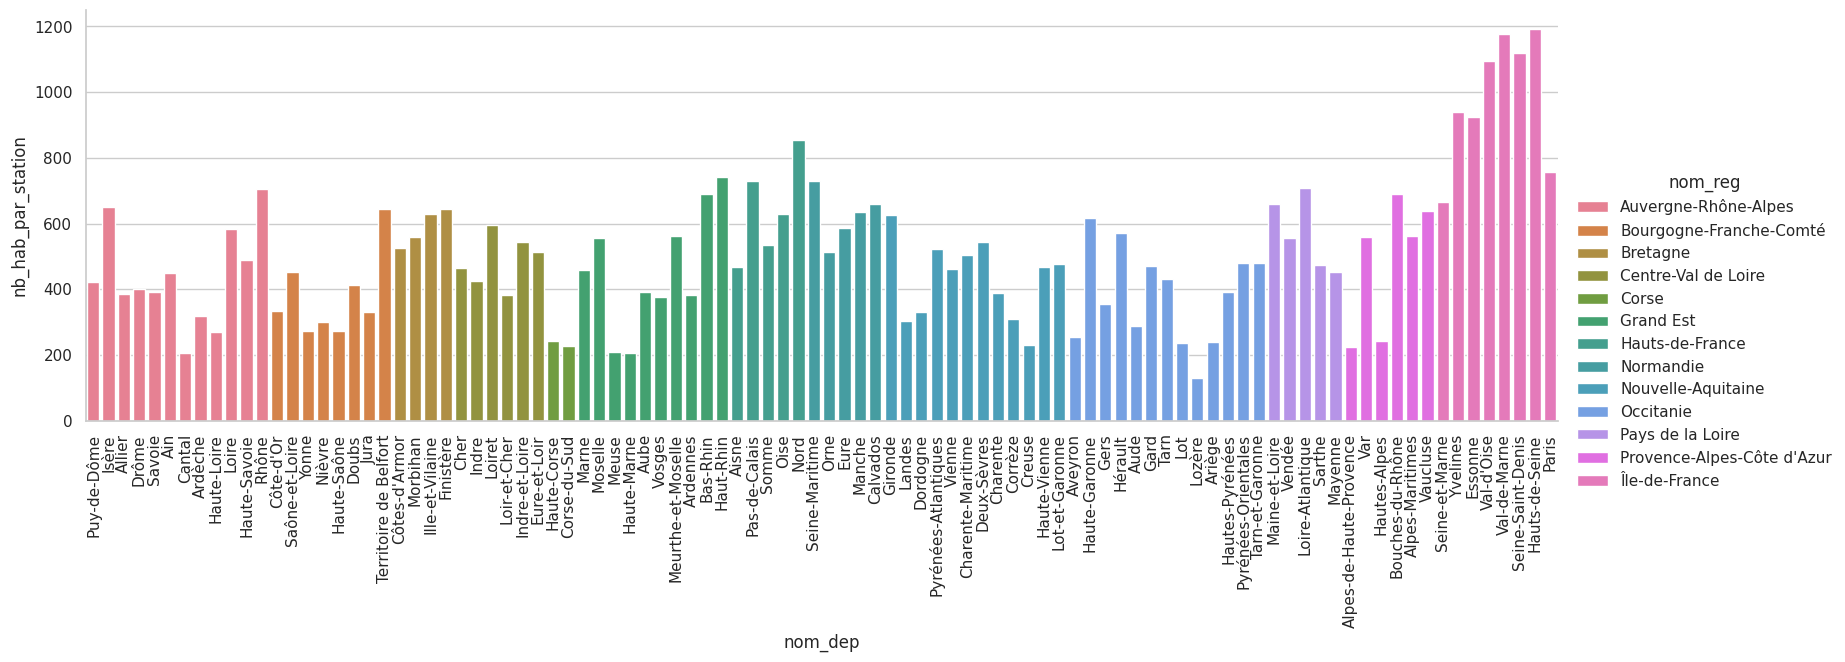
\includegraphics[width=0.9\paperwidth]{images/barplots/nb_hab_par_station_par_dep.png}
        \caption{\label{fig:nb_hap_par_stat_par_dep}Répartition du nombre d'habitants par station, en fonction du département}
    \end{figure}
\end{frame}

\begin{frame}{Nombre d'habitants par stations normalisé (1/2)}
    \begin{figure}
        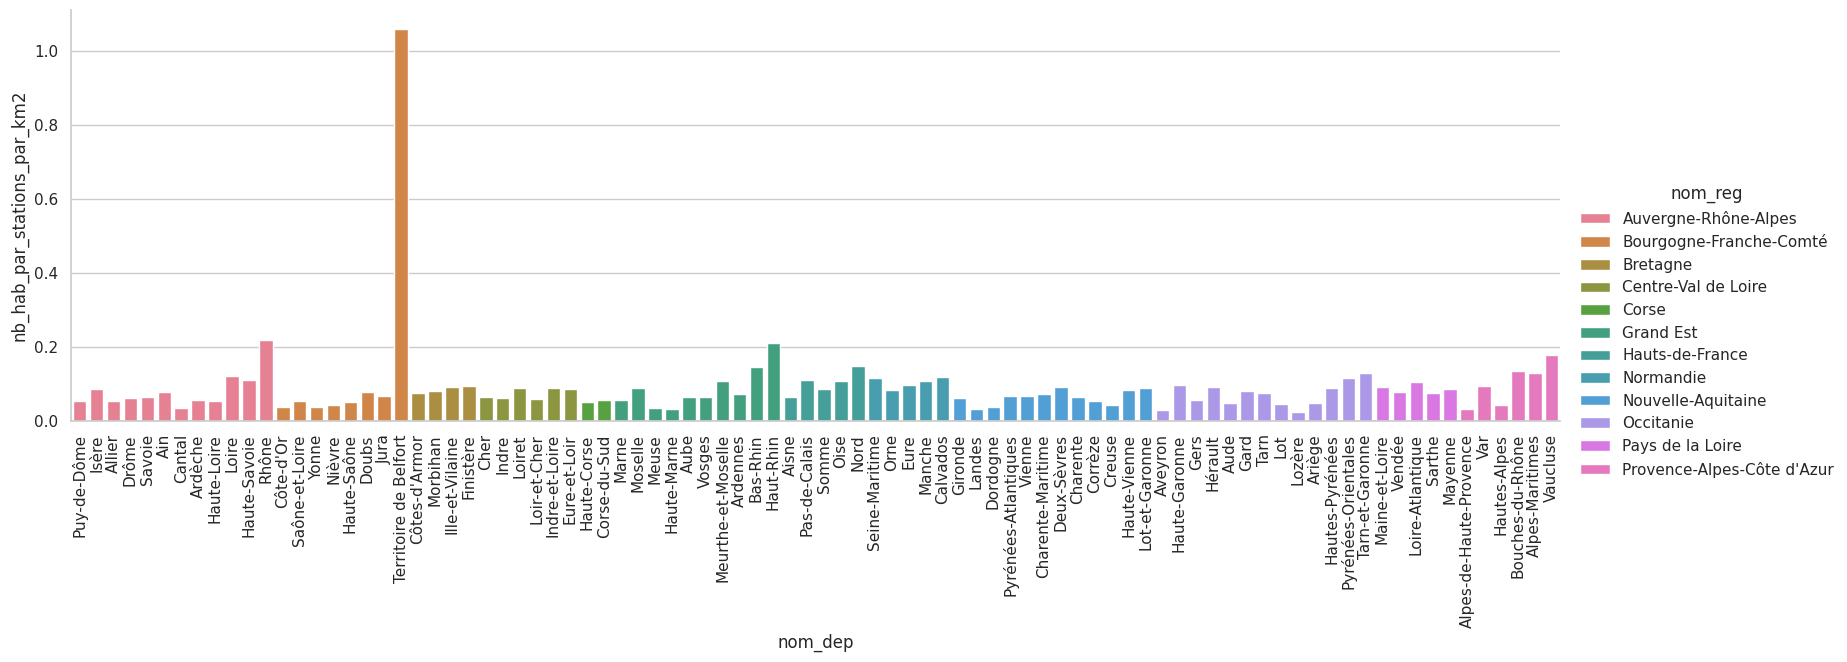
\includegraphics[width=0.9\paperwidth]{images/barplots/nb_hab_par_stations_par_km2_sansIDF.png}
        \caption{\label{fig:nb_hap_par_stat_par_dep_norm_ssIDF}Répartition du nombre d'habitants par station, en fonction du département (normalisé), sans l'Île-de-France}
    \end{figure}
\end{frame}

\begin{frame}{Nombre d'habitants par stations normalisé (2/2)}
    \begin{figure}
        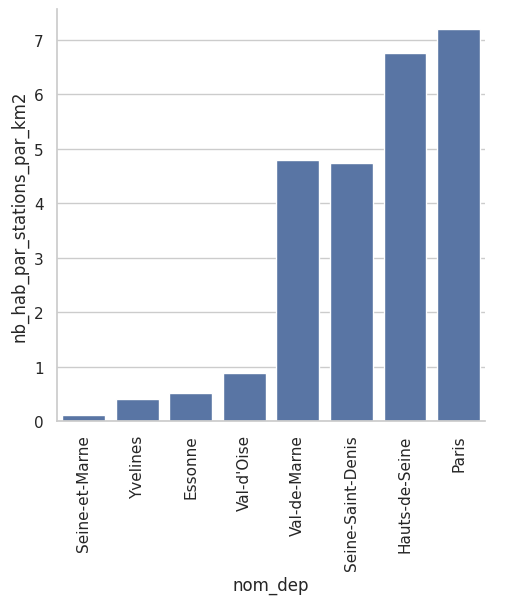
\includegraphics[height=0.55\paperheight]{images/barplots/nb_hab_par_stations_par_km2_IDF.png}
        \caption{\label{fig:nb_hap_par_stat_par_dep_norm_IDF}Répartition du nombre d'habitants par station, en fonction du département (normalisé), sur l'Île-de-France}
    \end{figure}
\end{frame}

\begin{frame}{Densité de stations (1/2)}
    \begin{figure}
        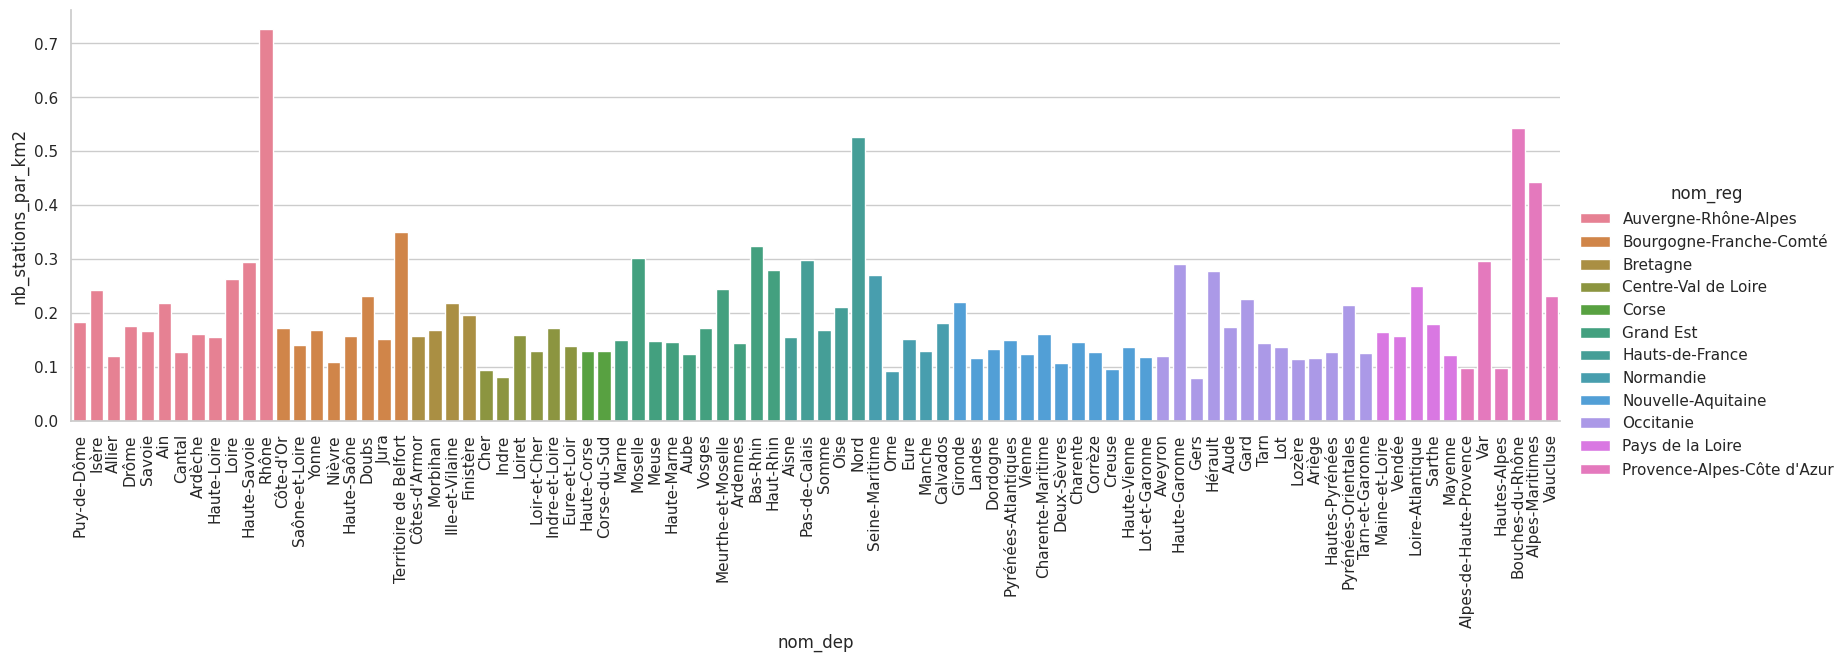
\includegraphics[width=0.9\paperwidth]{images/barplots/densite_station_par_dep_sansIDF.png}
        \caption{\label{fig:densite_stat_ssIDF}Nombre de stations de base au $\unit{km^2}$, sans l'Île-de-France}
    \end{figure}
\end{frame}

\begin{frame}{Densité de stations (2/2)}
    \begin{figure}
        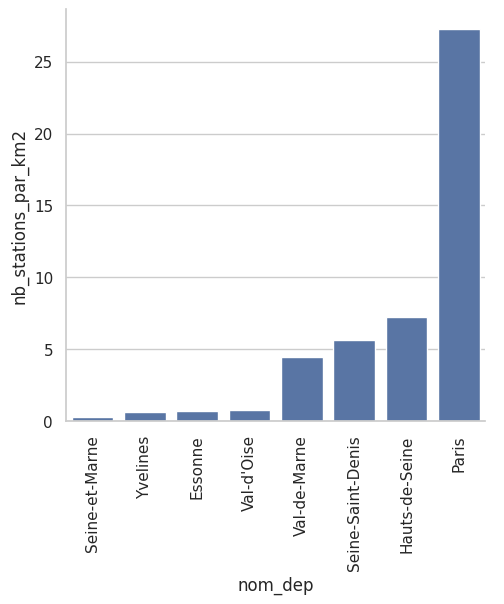
\includegraphics[height=0.55\paperheight]{images/barplots/densite_station_par_dep_IDF.png}
        \caption{\label{fig:densite_stat_IDF}Nombre de stations de base au $\unit{km^2}$, sur l'Île-de-France}
    \end{figure}
\end{frame}

\begin{frame}{Fréquences d'émission des stations 5G}
    \begin{figure}
        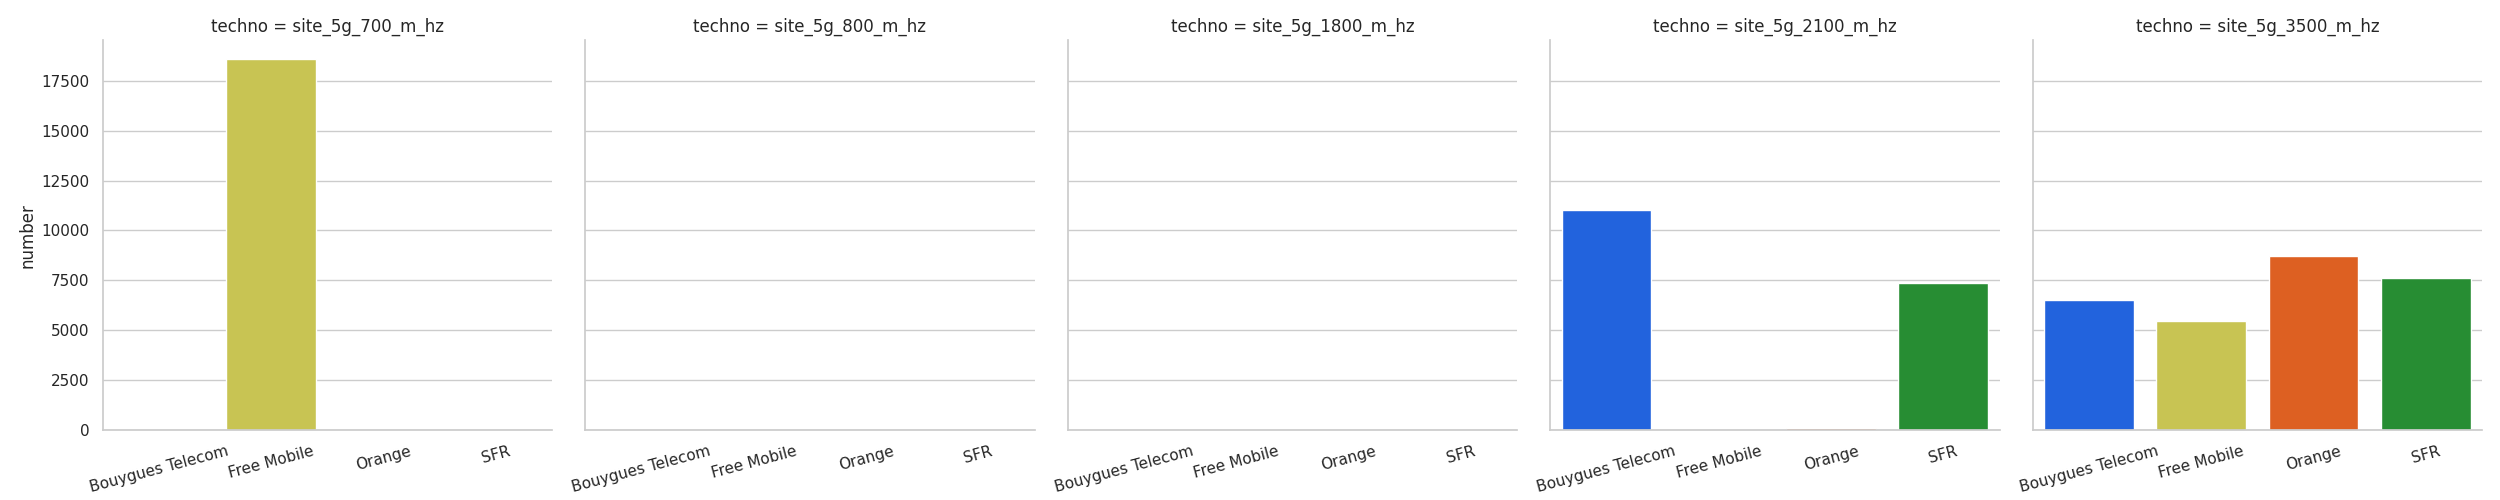
\includegraphics[width=0.9\paperwidth]{images/barplots/5G_freq.png}
        \caption{\label{fig:5g_freq}Répartition des fréquences d'émission des stations 5G, en fonction des opérateurs}
    \end{figure}
\end{frame}

\subsection{Détection de voisins - méthode PAQUIRY}
\insertsubsectionframe

\begin{frame}{Principe général}
    La recherche de voisins va s'articuler atour de deux axes :
    \begin{block}{Triangulation de Delaunay}
        On crée un graphe de voisinage grâce à la triangulation de Delaunay. Ceci nous donne donc, pour chaque station de base, une liste de voisins potentiels.
        Il faut ensuite vérifier que ce sont bien des voisins réels.
    \end{block}
    \begin{block}{Critères de sélection}
        Pour être sûr qu'un voisin est un voisin réel on applique trois critères, dans l'ordre suivant :
        \begin{enumerate}
            \item la distance maximale ;
            \item le plus proche voisin dans un cadrant ;
            \item l'angle minimum entre deux voisins.
        \end{enumerate}
    \end{block}
    Cette méthode a été élaborée par Delphine PAQUIRY l'été dernier.
\end{frame}

\begin{frame}{Critère de distance}
    \begin{columns}
        \begin{column}{0.4\paperwidth}
            \begin{block}{Principe}
                Ici, on élimine tous les voisins qui sont distants de plus de $\unit[15]{km}$.
            \end{block}
            \begin{block}{Intérêt du critère}
                Il est logique de penser que deux stations trop éloignées géographiquement ne sont pas voisines.
            \end{block}
        \end{column}
        \begin{column}{0.55\paperwidth}
            \begin{figure}
                \boxed{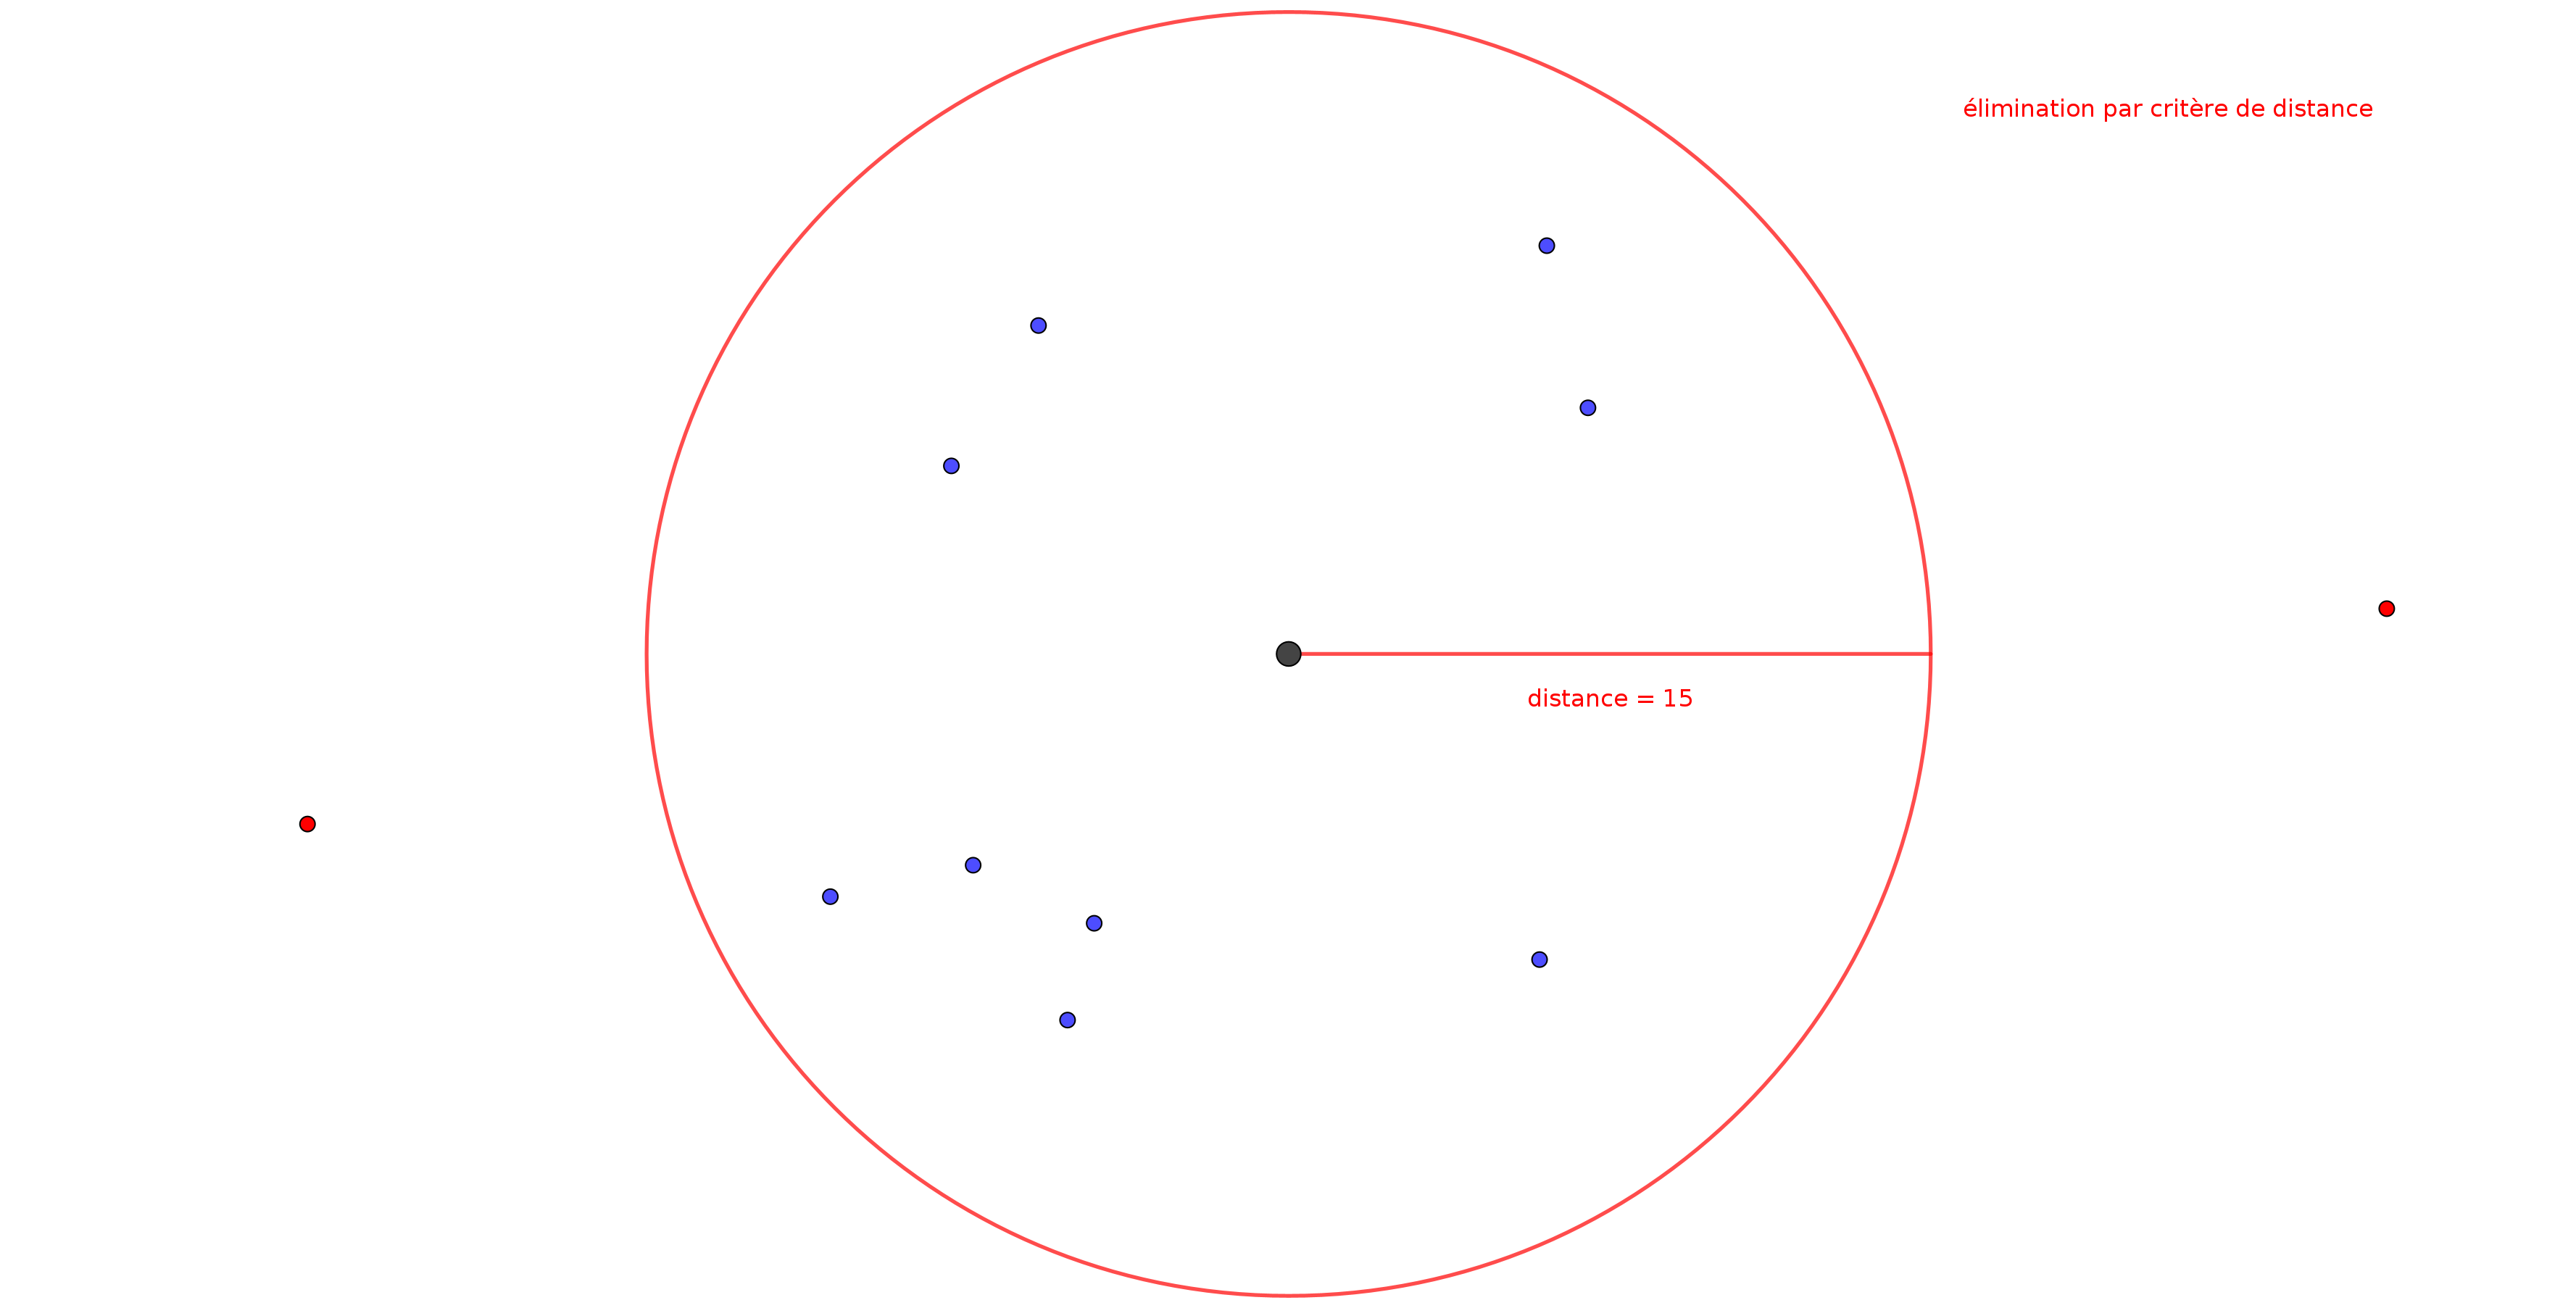
\includegraphics[width=0.5\paperwidth]{images/criteria_illustrations/distance.png}}
                \caption{\label{fig:distance_crit}Illustration du critère de distance}
            \end{figure}
        \end{column}
    \end{columns}
\end{frame}

\begin{frame}{Critère des cadrants}
    \begin{columns}
        \begin{column}{0.4\paperwidth}
            \begin{block}{Principe}
                Ici, on ne garde que le plus proche voisin dans un cadrant. On a choisi 6 cadrants car c'est le chiffre qui nous donne les meilleurs résultats.
            \end{block}
            \begin{block}{Intérêt du critère}
                On évite les effets de cluster.
            \end{block}
        \end{column}
        \begin{column}{0.55\paperwidth}
            \begin{figure}
                \boxed{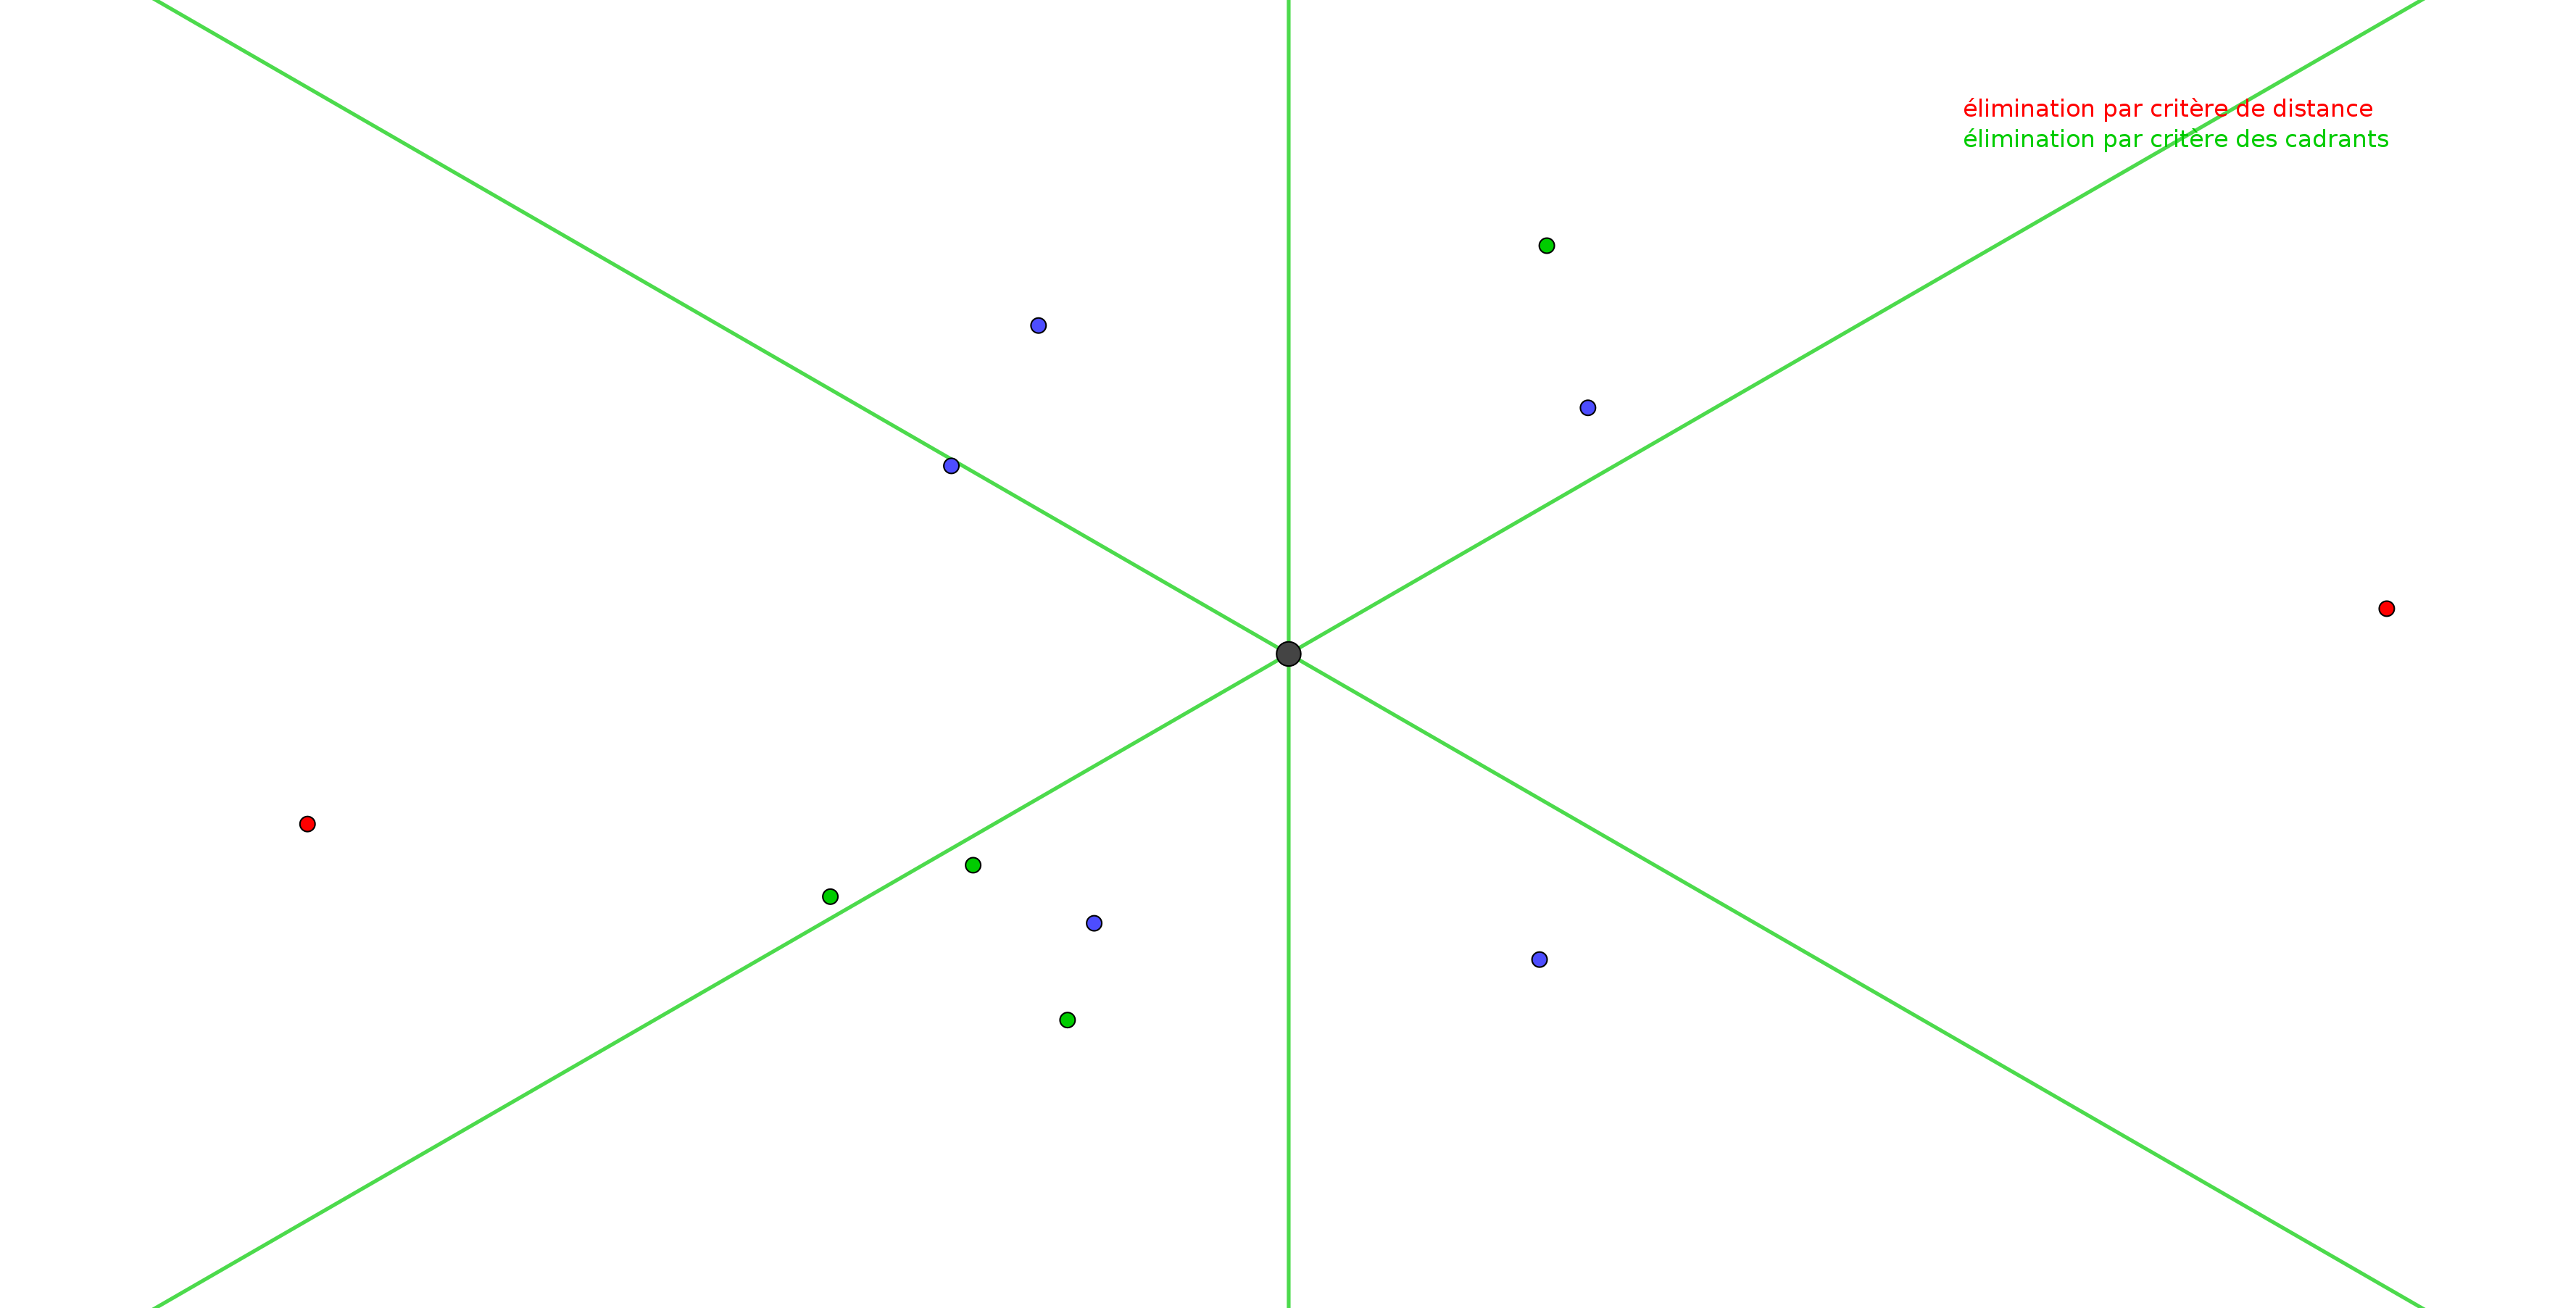
\includegraphics[width=0.5\paperwidth]{images/criteria_illustrations/cadrants.png}}
                \caption{\label{fig:cadrants_crit}Illustration du critère des cadrants}
            \end{figure}
        \end{column}
    \end{columns}
\end{frame}

\begin{frame}{Critère de l'angle}
    \begin{columns}
        \begin{column}{0.4\paperwidth}
            \begin{block}{Principe}
                Ici, si deux voisins sont séparés d'un angle inférieur à $30^{\circ}$, on ne garde que le plus proche. Cette valeur d'angle est arbitraire et pourrait être variable en fonction de l'urbanité de la station.
            \end{block}
            \begin{block}{Intérêt du critère}
                Si deux stations sont trop proches angulairement parlant, la plus proche fait écran par rapport à la plus éloignée.
            \end{block}
        \end{column}
        \begin{column}{0.55\paperwidth}
            \begin{figure}
                \boxed{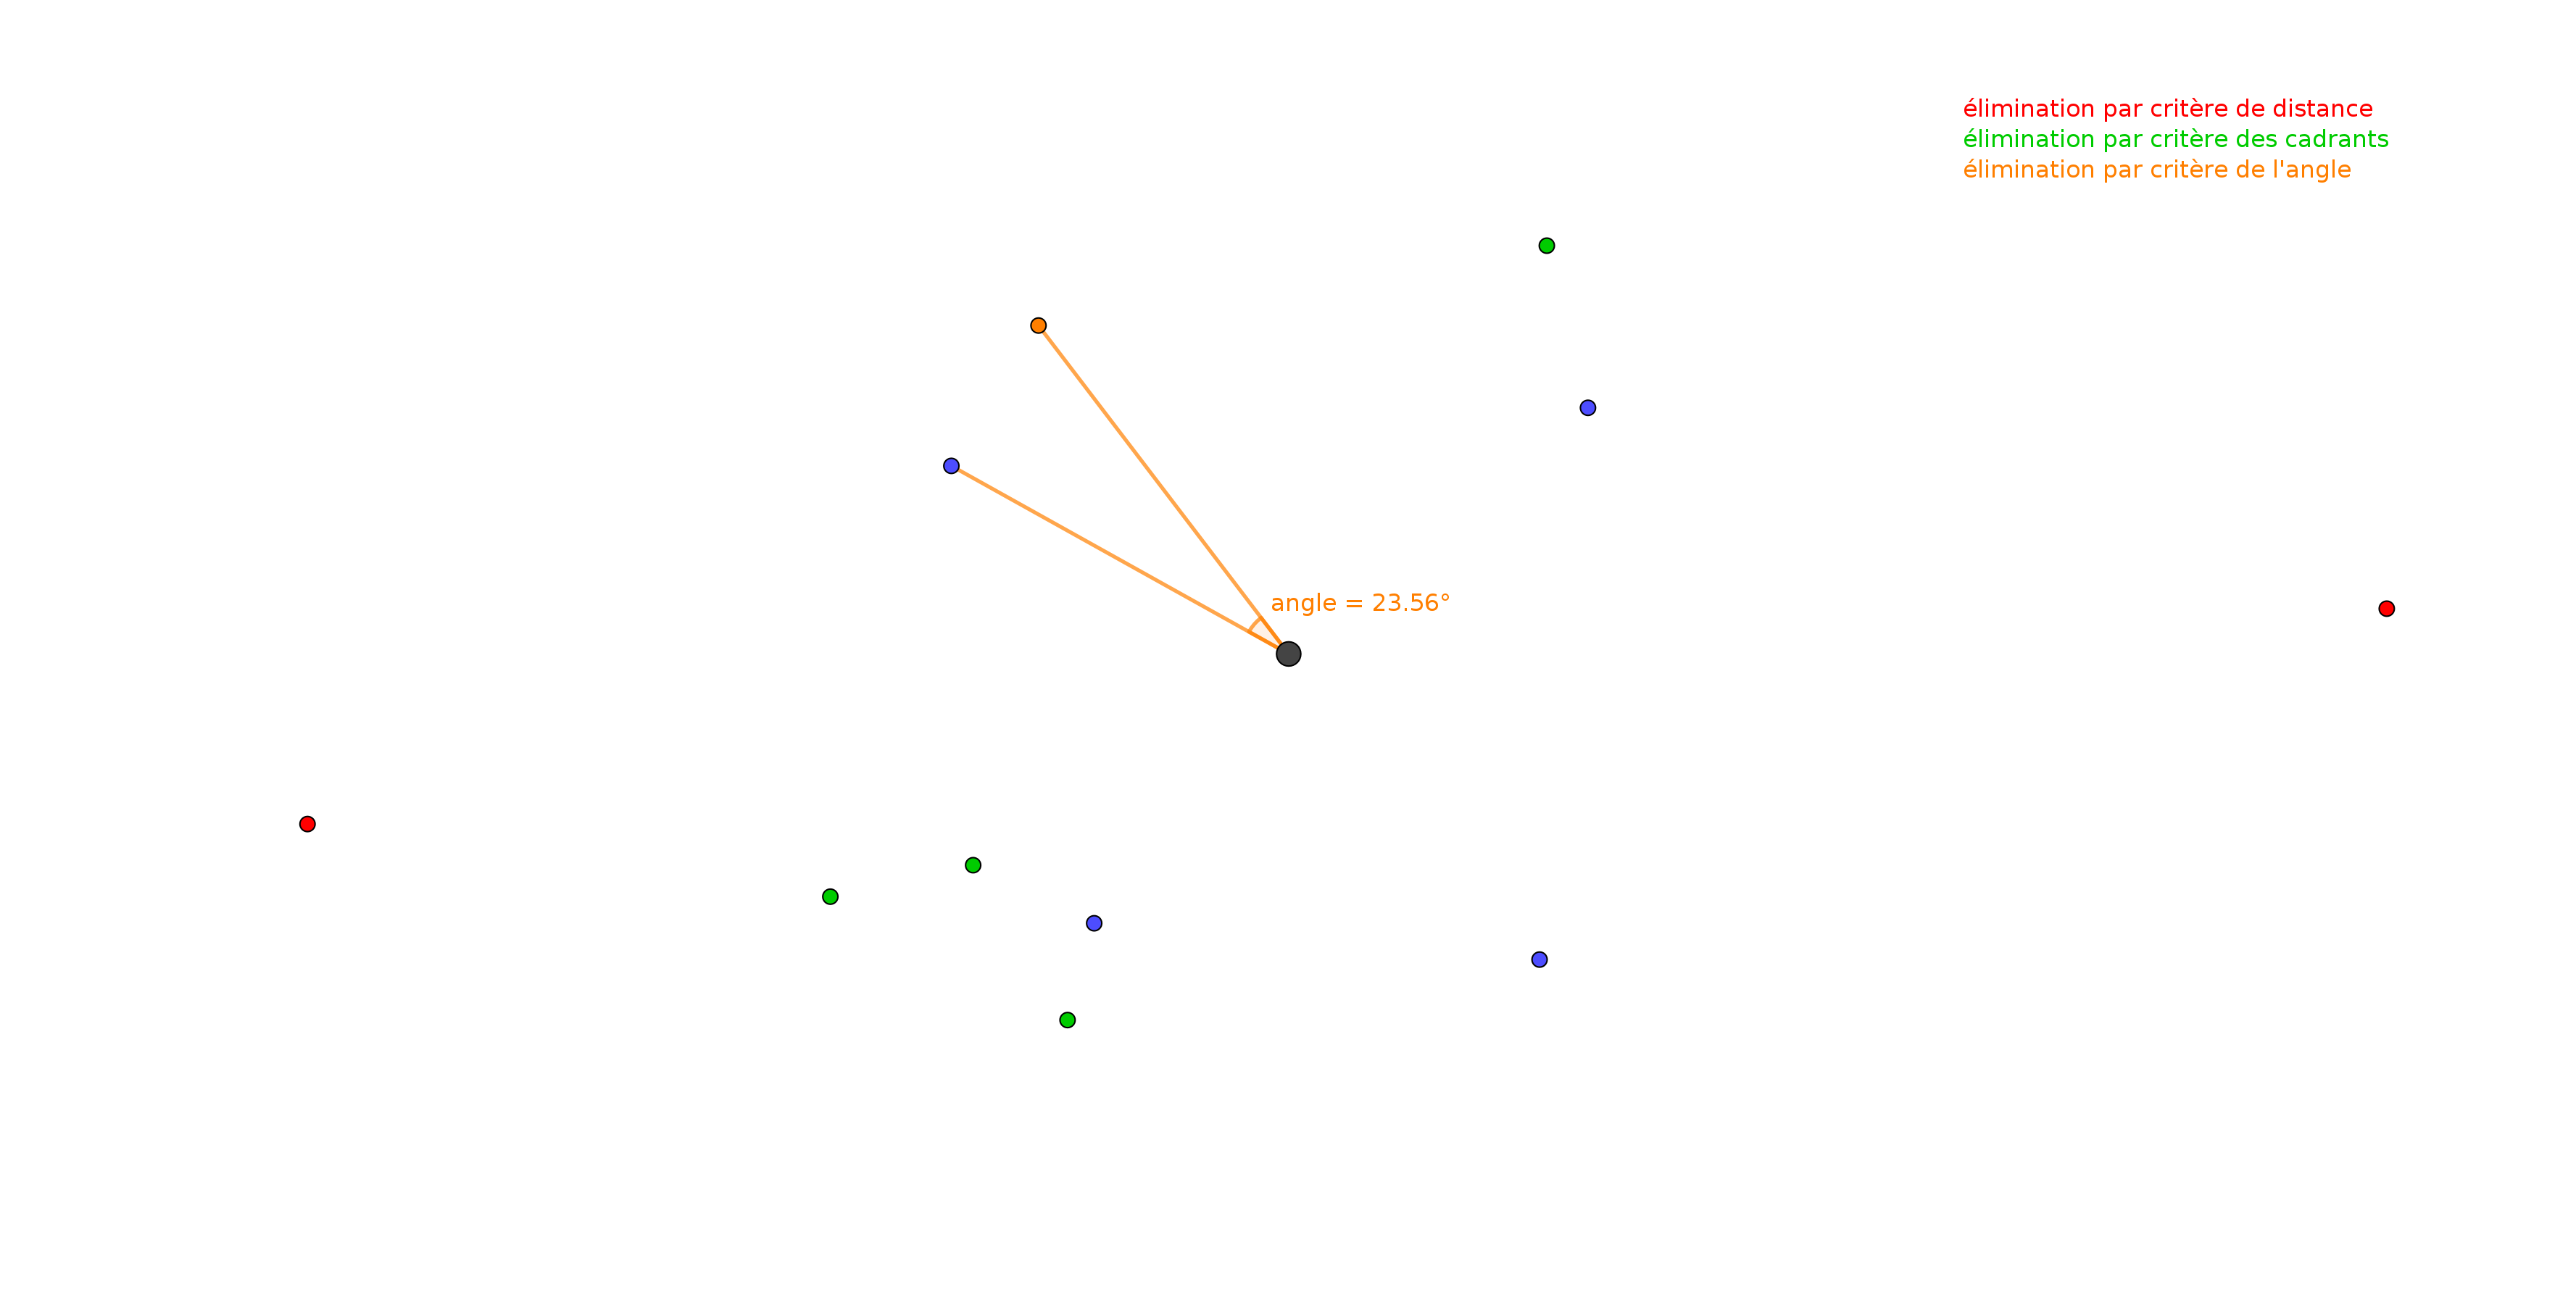
\includegraphics[width=0.5\paperwidth]{images/criteria_illustrations/angle.png}}
                \caption{\label{fig:angle_crit}Illustration du critère de l'angle}
            \end{figure}
        \end{column}
    \end{columns}
\end{frame}

\begin{frame}{Voisins réels}
    Voici donc ce que l'on obtient à la fin, un graphe de voisinage :
    \begin{figure}
        \boxed{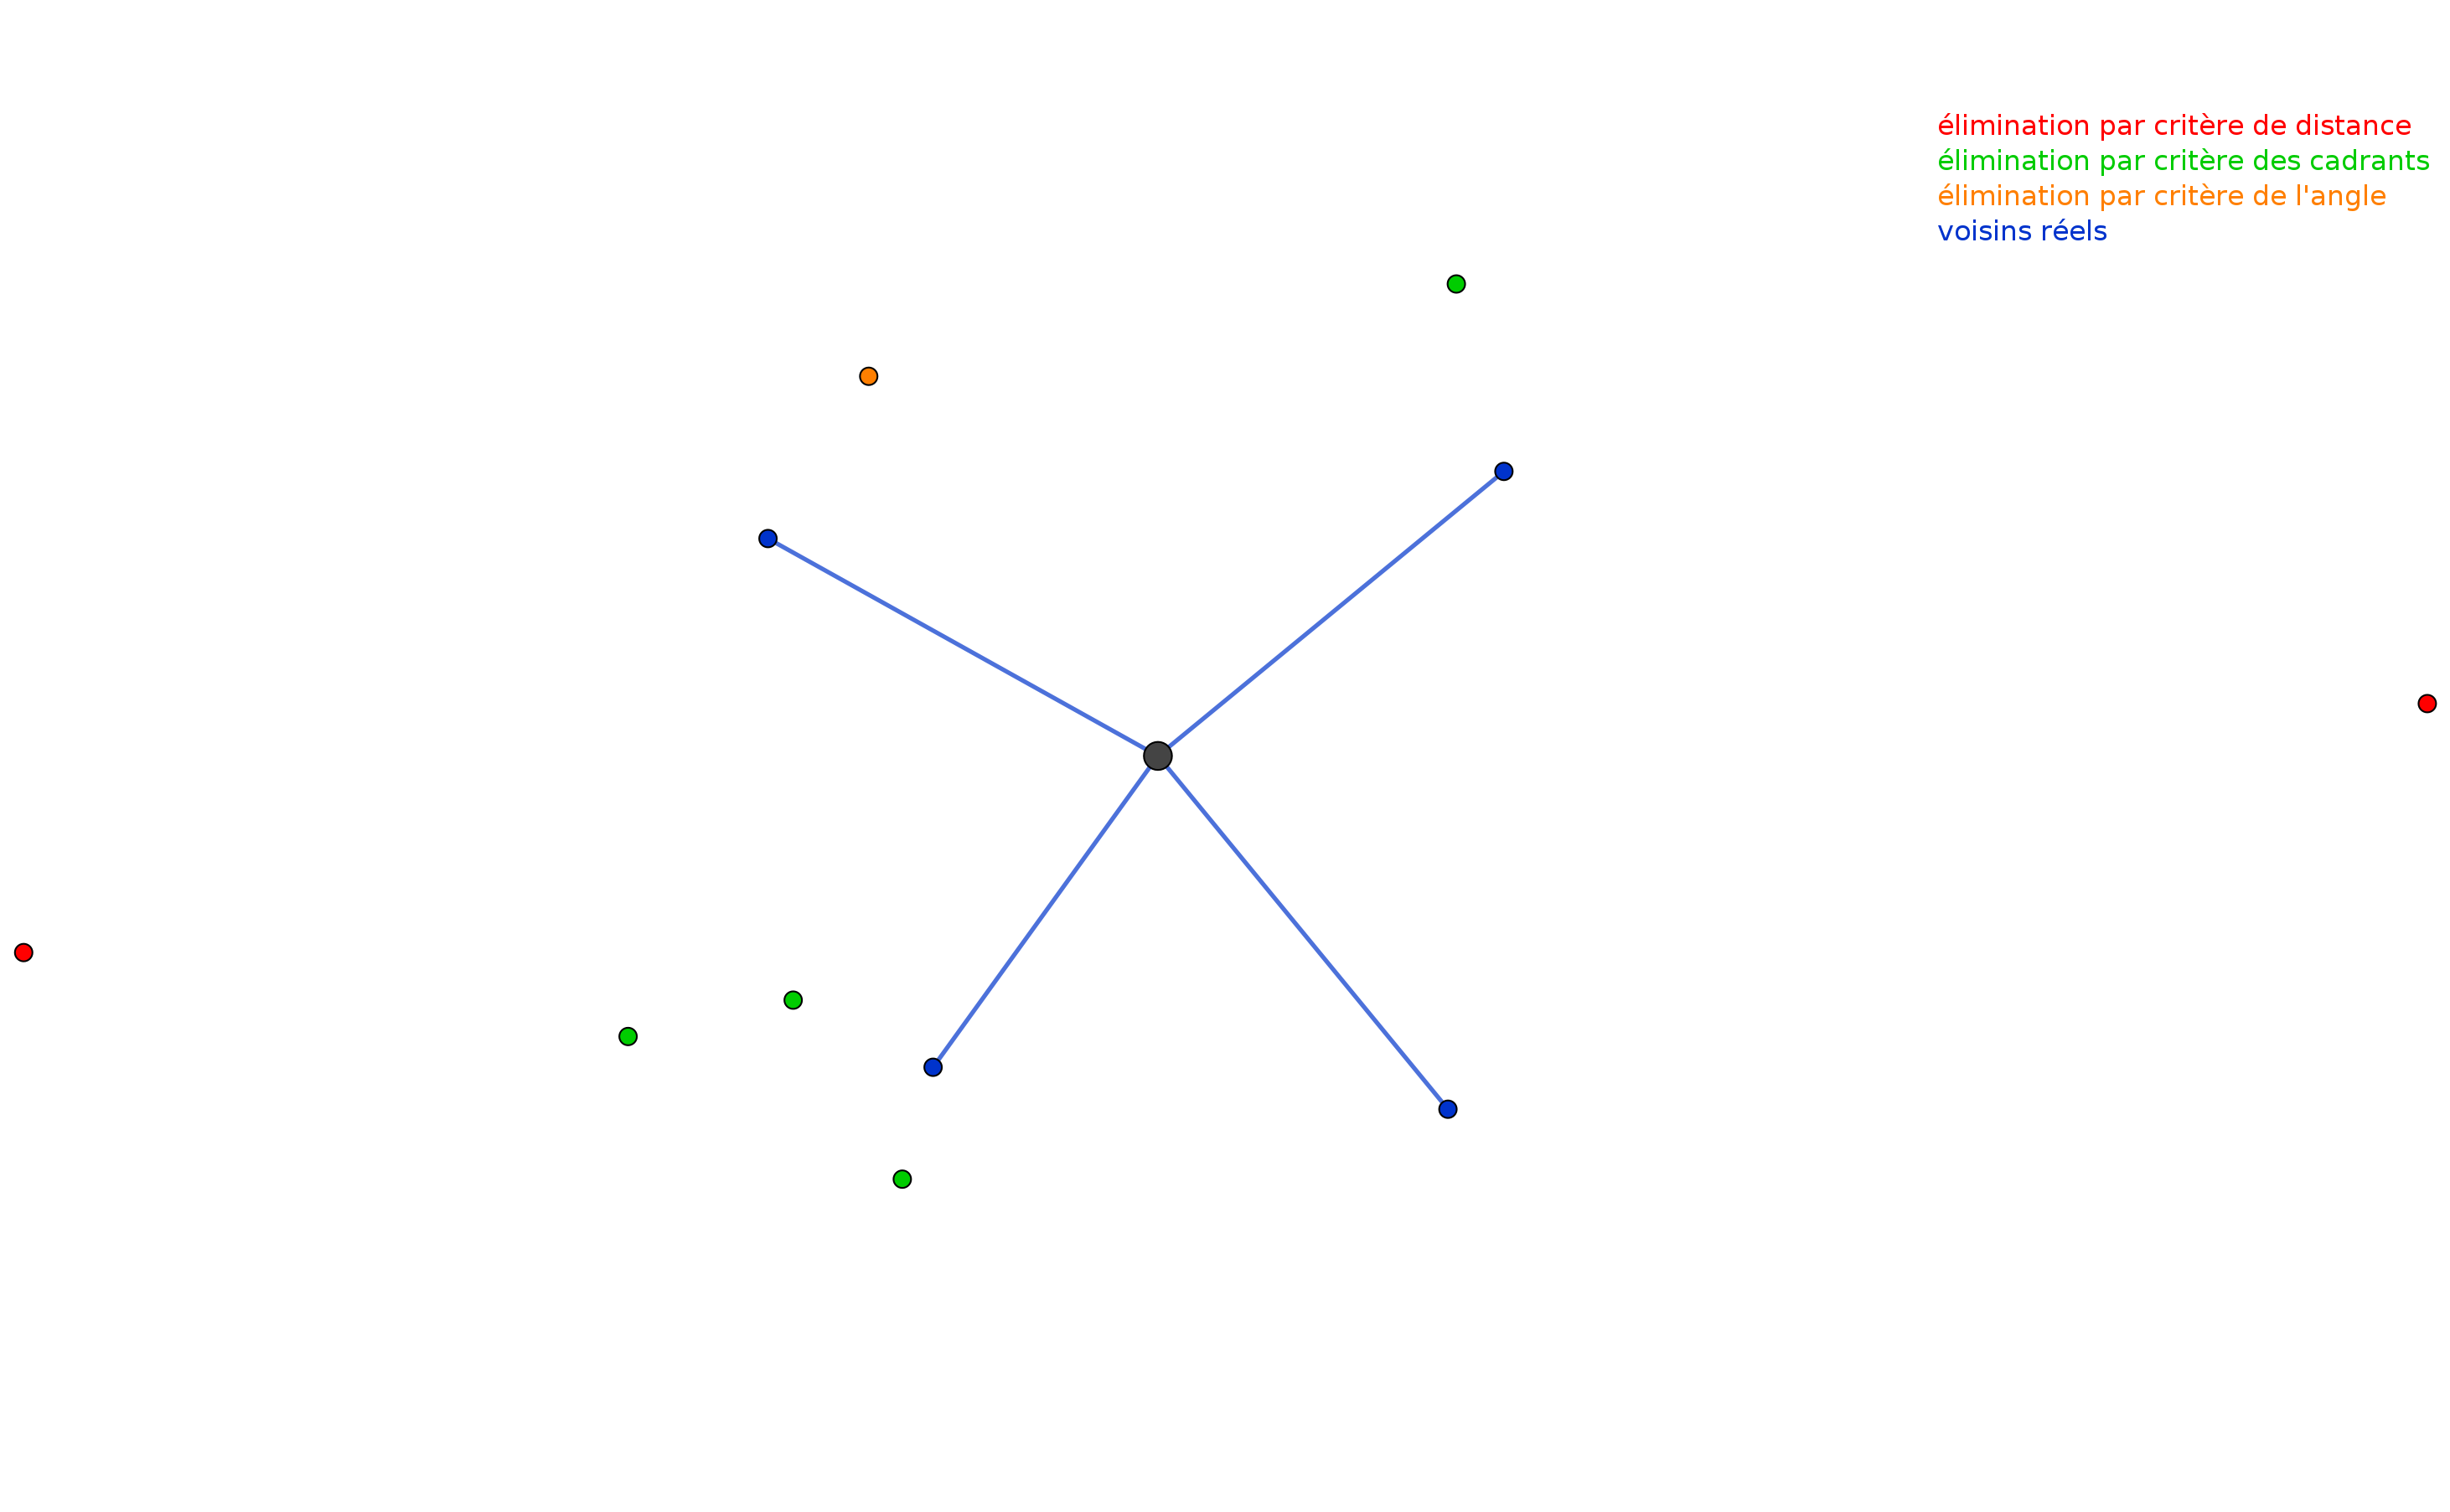
\includegraphics[height=0.55\paperheight]{images/criteria_illustrations/final.png}}
        \caption{\label{fig:result_crit}Résultat final - voisins réels}
    \end{figure}
\end{frame}

\subsection{Détection automatique des villes}
\insertsubsectionframe

\begin{frame}{DBScan}
    \begin{block}{Principe}
        \begin{itemize}
            \item Méthode de référence de la classification à densité (détection de clusters en se basant sur la concentration de points);
            \item Se base sur deux paramètres : $\varepsilon$ et $n_{min}$ qui caractérisent respectivement la distance maximale pour que deux points soient considérés \og proches \fg{} et la quantité minimale de points proches pour qu'un cluster soit créé.
        \end{itemize}
    \end{block}

    \begin{block}{Inconvénients}
        \begin{itemize}
            \item Le choix du paramètre $\varepsilon$ est hasardeux;
            \item Ne se comporte pas bien avec des jeux de données avec des clusters de densité variable (certains clusters avec des points plus rapprochés que d'autres);
            \item Réagit mal au bruit;
            \item Est binaire : un point appartient ou n'appartient pas à un cluster, pas d'entre deux.
        \end{itemize}
    \end{block}
\end{frame}

\begin{frame}{Fonctionnement DBScan (1/2)}

    \begin{columns}
        \begin{column}{0.40\textwidth}
            \begin{block}{Etape 0 : Initialisation}
                Soient n points de $\mathbb{R}^p$, $\epsilon \in \mathbb{R}$ et $n_{min} \in \mathbb{N}$.

                Ici, on prend $n_{min}=3$ et $\epsilon=2$
            \end{block}

            \begin{block}{Etape 1 - Les voisins}
                Pour chaque point, on cherche tous les points à une distance inférieure à $\epsilon$ (dont lui même). On les appelera les voisins.
            \end{block}
        \end{column}

        \begin{column}{0.60\textwidth}
            \begin{figure}
                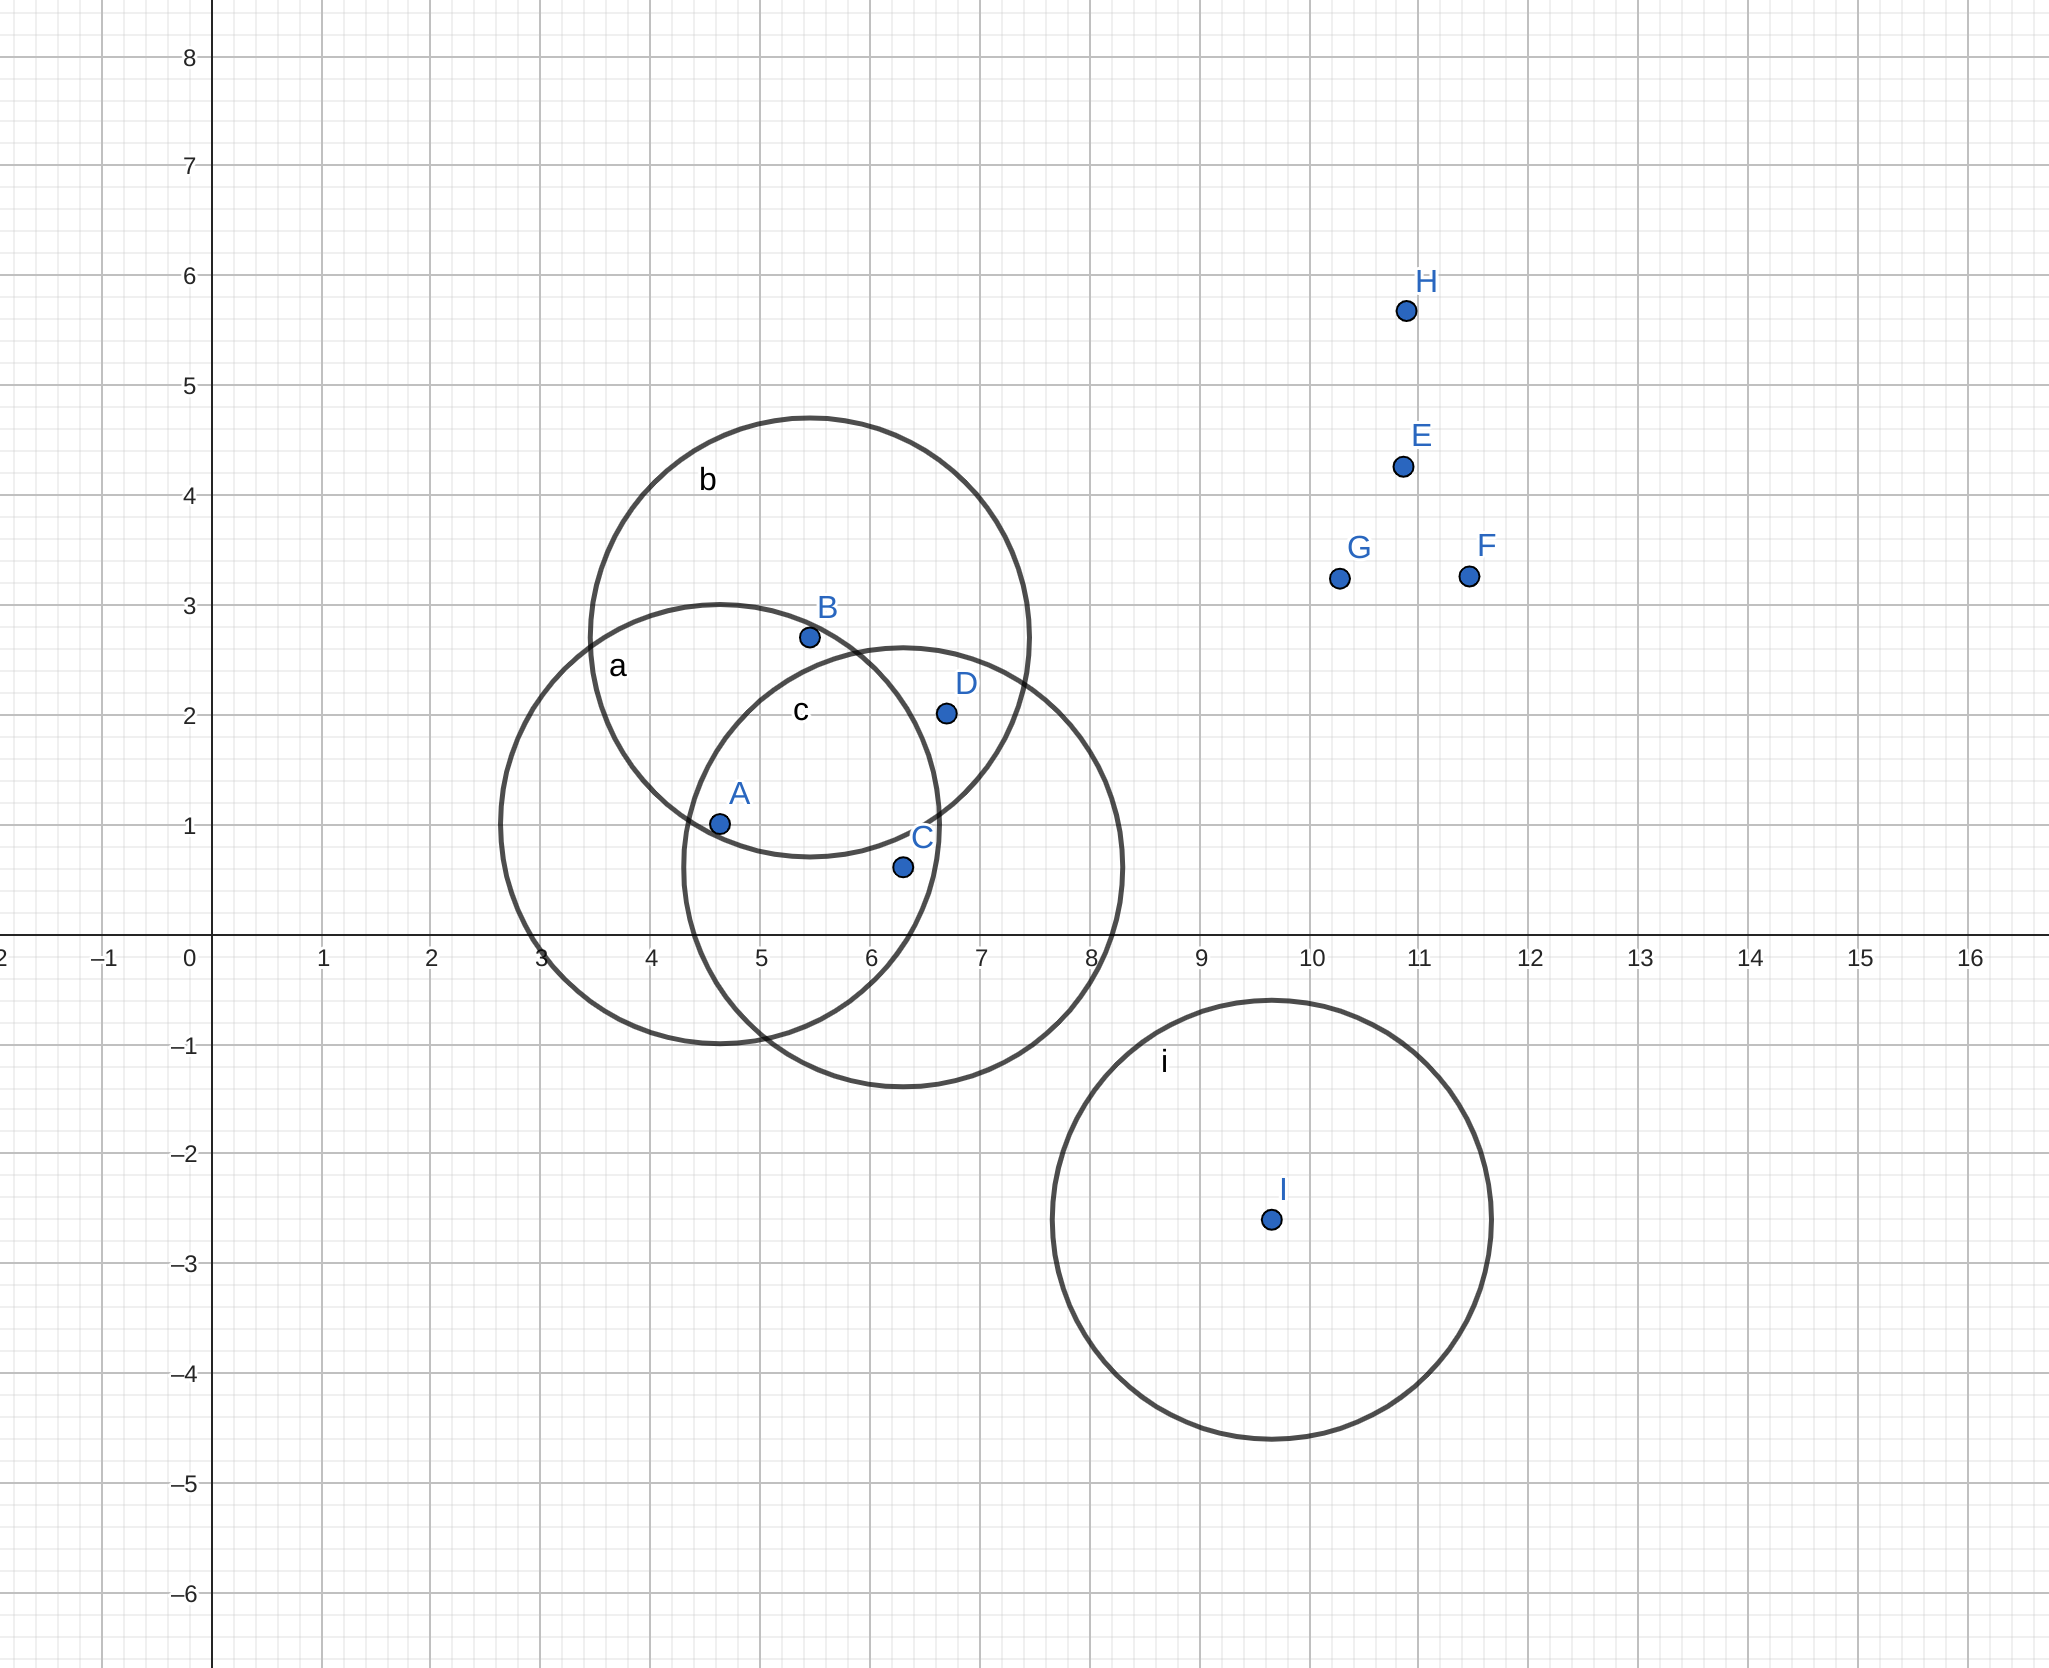
\includegraphics[height=0.41\paperheight]{images/Illustration_DBScan_1.png}
                \caption{\label{fig:ill_DBScan_1} DBScan : Détection des voisins}
            \end{figure}
        \end{column}
    \end{columns}

    \begin{table}[!ht]
        \centering
        \begin{tabular}{c|ccccc}
            \textbf{Point} & \textbf{A} & \textbf{B} & \textbf{C} & \textbf{\dots} & \textbf{I} \\ \hline
            \textbf{N(Points)} & $\left\{ A, B, C \right\}$ & $\left\{ A, B, D \right\}$ & $\left\{ A, C, D \right\}$ & & $\left\{ I \right\}$ \\ 
        \end{tabular}
    \end{table}
\end{frame}

\begin{frame}{Fonctionnement DBScan (2/2)}
    \begin{columns}
        \begin{column}{0.55\textwidth}
            \begin{block}{Etape 2 - Constuction du graphe de voisinage des noyaux}
                \begin{itemize}
                    \item Les points ayant au moins $n_{min}$ voisins sont considérés comme des noyaux. On construit alors un graphe dont les sommets sont les noyaux et il existe une arete entre deux noyaux si et seulement si ils sont voisins.
                    \item Les composantes connexes de ce graphe sont les clusters. On rattache alors aux clusters les points voisins d'au moins un noyau de ce cluster, on les appelle points de bordure.
                    \item Enfin, les sommets qui n'apparaissent pas dans le graphe sont considérés comme du bruit (pas de classe).
                \end{itemize}
            \end{block}
        \end{column}
        \begin{column}{0.45\textwidth}
            \begin{figure}
                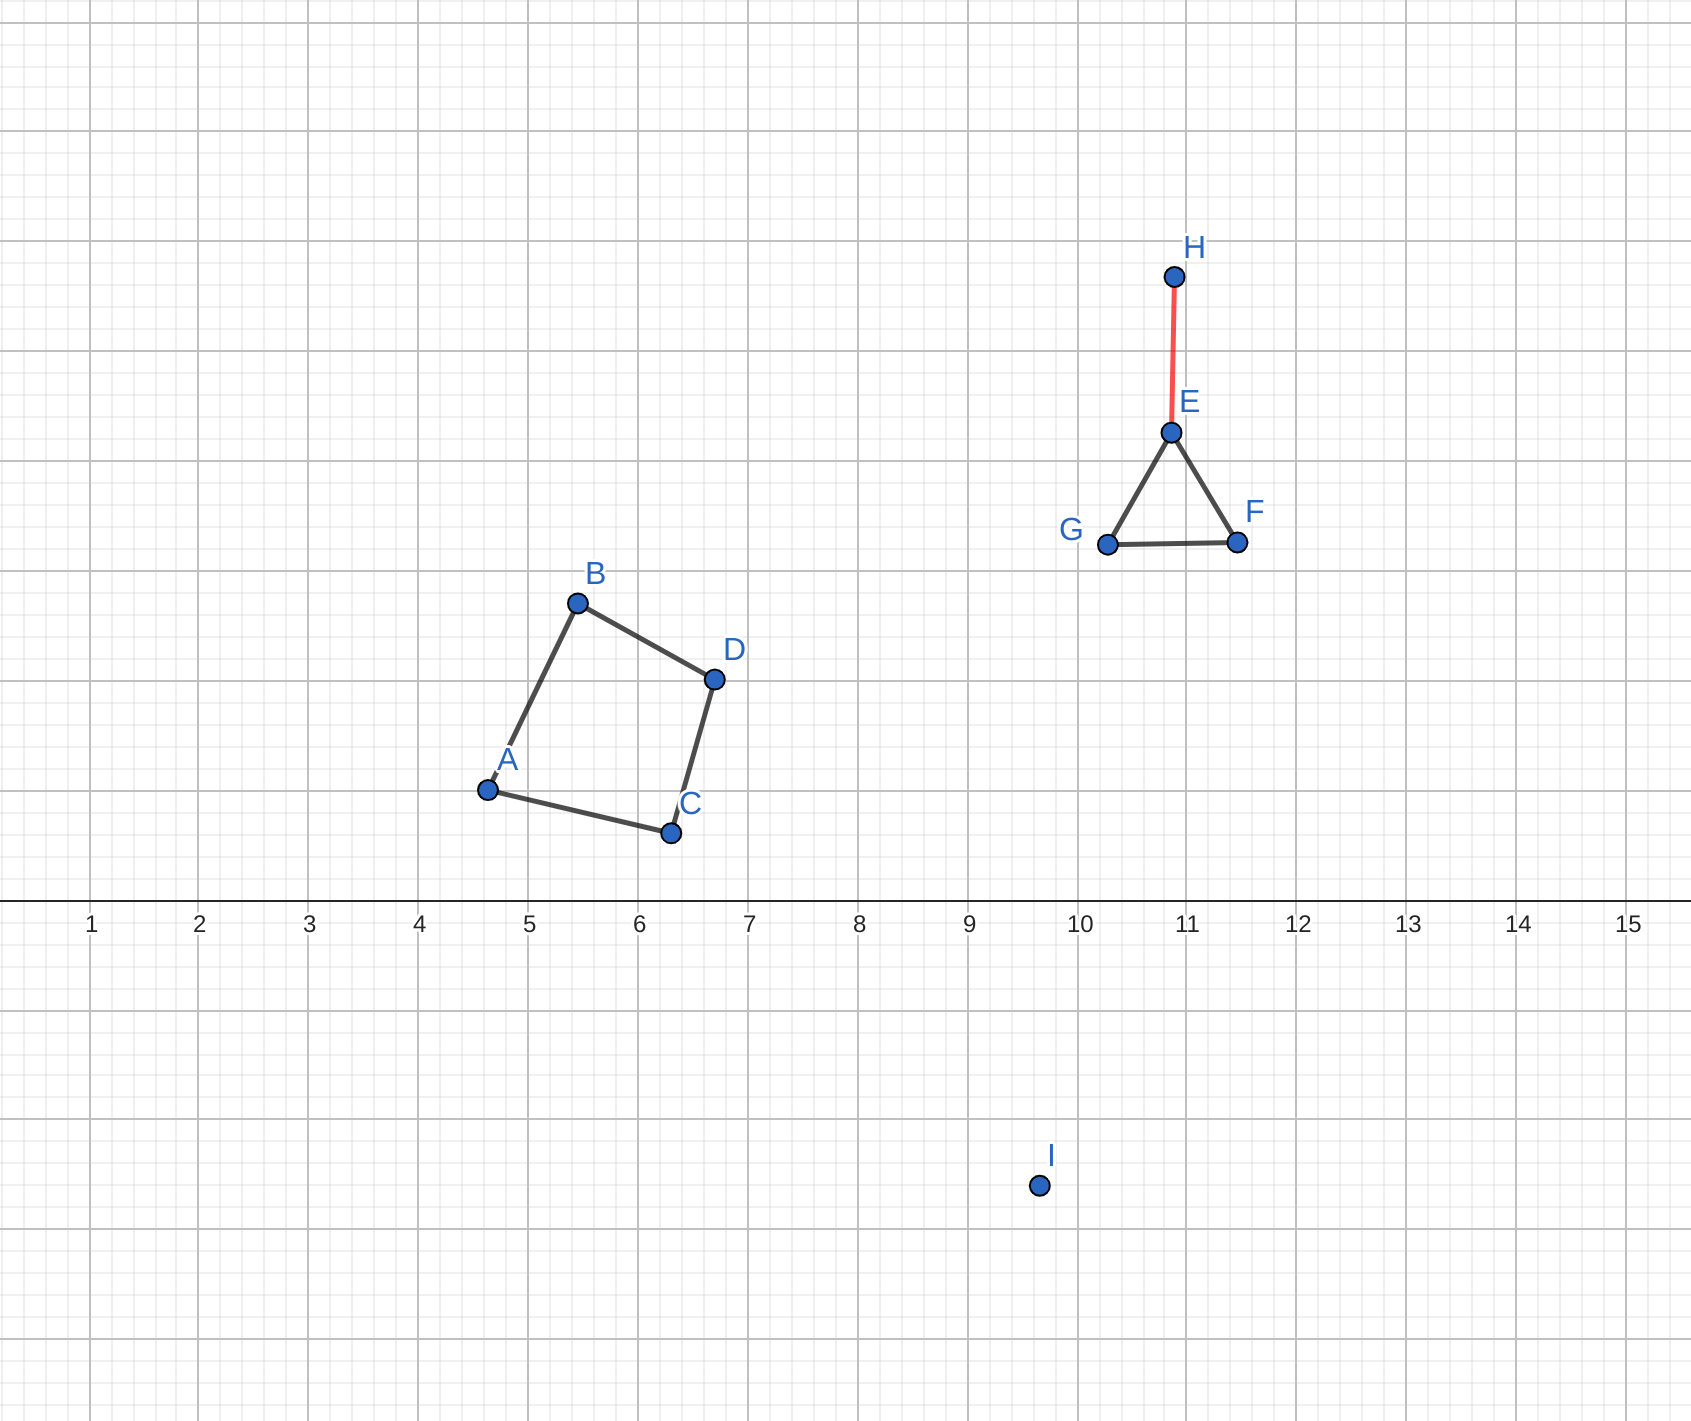
\includegraphics[height=0.5\paperheight]{images/Illustration_DBScan_2.png}
                \caption{\label{fig:ill_DBScan_2} DBScan : création des clusters}
            \end{figure}
        \end{column}
    \end{columns}
\end{frame}

\begin{frame}{Changement de métrique}
    Une façon d'améliorer le problème de mauvaise prise en compte du bruit est de changer de métrique :
    \begin{columns}
        \begin{column}{0.55\textwidth}
            \begin{block}{\emph{Core distance}}
                La \emph{core distance} d'un point du jeu de donnée est la distance entre ce point et son $k$-ième plus proche point ($k$ à fixer).
            \end{block}
        
            \begin{block}{Nouvelle métrique}
                La distance entre deux points $x$ et $y$ d'un jeu de donnée peut être définie comme la plus grande valeur entre les \emph{core distances} de $x$ et $y$ et la distance eucliedienne entre $x$ et $y$.
            \end{block}
        \end{column}
        \begin{column}{0.4\textwidth}
            \begin{figure}
                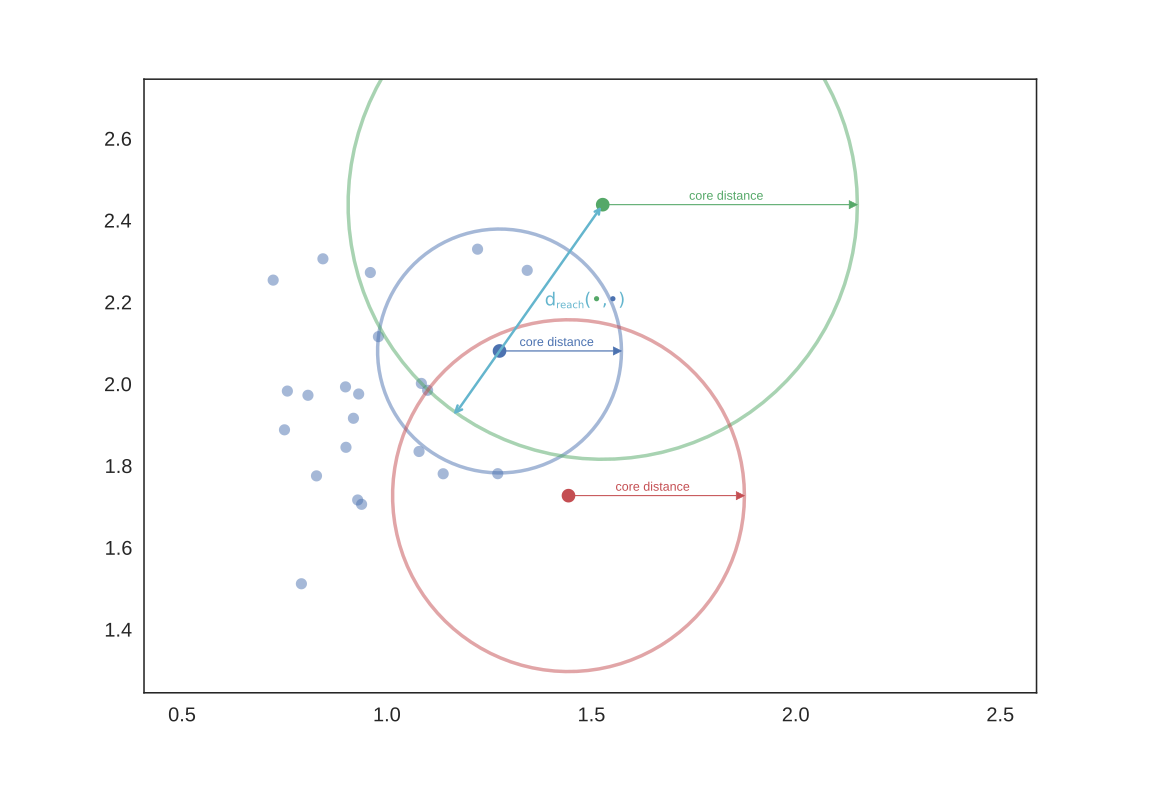
\includegraphics[width=0.6\paperheight]{images/metrique.png}
                \caption{\label{fig:metrique}Nouvelle métrique}
            \end{figure}
        \end{column}
    \end{columns}
\end{frame}



\begin{frame}{Fonctionnement HDBScan\footnotemark[2] }
    \begin{block}{Principe général}
        HDBScan consiste à fusionner les méthodes de classification hierarchique adscendante et DBScan pour permettre de s'affranchir du paramètre $\varepsilon$.
    \end{block}


    \begin{figure}
        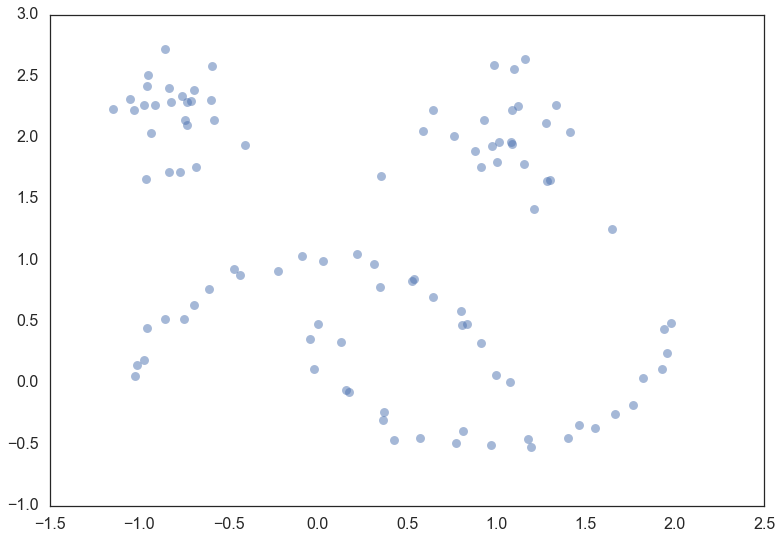
\includegraphics[width=0.5\paperheight]{images/Illustration-HDBSCAN-1.png}
        \caption{\label{fig:ill_HDBScan_1}Le jeu de donnée exemple \footnotemark[3]}
    \end{figure}

    \footnotetext[2]{\url{http://link.springer.com/chapter/10.1007\%2F978-3-642-37456-2\_14}}
    \footnotetext[3]{\url{{https://hdbscan.readthedocs.io/en/latest/how\_hdbscan_works.html}}}
\end{frame}

\begin{frame}{Fonctionnement HDBScan }
    \begin{columns}
        \begin{column}{0.55\textwidth}
            \begin{block}{Etape 1 - Constuction de l'abre couvrant de poids minimum}
                \begin{itemize}
                    \item Représenter les données par un graphe complet où chaque point est un sommet
                    \item Valuer les arêtes par la métrique expliquée précédemment;
                    \item Trouver un arbre couvrant de poids minimum dans ce graphe;
                \end{itemize}
            \end{block}
        \end{column}
        \begin{column}{0.45\textwidth}
            \begin{figure}
                \includegraphics[height=0.4\paperheight]{images/Illustration-HDBScan-2.png}
                \caption{\label{fig:ill_HDBScan_2} Arbre couvrant de poids minimum}
            \end{figure}
        \end{column}
    \end{columns}
\end{frame}

\begin{frame}{Fonctionnement HDBScan }
    \begin{columns}
        \begin{column}{0.55\textwidth}
            \begin{block}{Etape 2 - Création du dendrogramme}
                \begin{itemize}
                    \item Ne garder que les arêtes correspondant à un certain seuil que l'on fait varier.
                    \item Observer l'évolution des classes (composantes connexes) en fonction de cette distance.
                    \item Construire un dendrogramme à partir de ces informations.
                \end{itemize}
            \end{block}
        \end{column}
        \begin{column}{0.45\textwidth}
            \begin{figure}
                \includegraphics[height=0.4\paperheight]{images/Illustration-HDBScan-3.png}
                \caption{\label{fig:ill_HDBScan_3} Dendrogramme}
            \end{figure}
        \end{column}
    \end{columns}
\end{frame}

\begin{frame}{Fonctionnement HDBScan }
    \begin{columns}
        \begin{column}{0.55\textwidth}
            \begin{block}{Etape 3 - Condensation du dendrogramme}
                    On va chercher à condenser le dendrogramme précédent. Pour cela, on considère qu'au départ il n'y a qu'un cluster.
                    On considère qu'un cluster n'est plus considéré comme tel quand il possède moins d'individu qu'un certain seuil (appelons le $n_{min}$).
                    A chaque séparation dans le dendrogramme, il y'a trois cas de figure :
                    \begin{itemize}
                        \item Si les deux parties comportent au moins $n_{min}$ individus, alors on considère que le cluster parent meurt et donne naissance à deux enfants.
                        \item Si une seule des parties comporte au moins $n_{min}$ individus, alors on considère que ce cluster est la continuation du précédent.
                        \item Si les deux parties comportent moins de $n_{min}$ individus, alors on considère que le cluster meurt.
                    \end{itemize}

            \end{block}
        \end{column}
        \begin{column}{0.45\textwidth}
            \begin{figure}
                \includegraphics[height=0.4\paperheight]{images/Illustration-HDBScan-4.png}
                \caption{\label{fig:ill_HDBScan_4} Dendrogramme condensé}
            \end{figure}
        \end{column}
    \end{columns}
\end{frame}

\begin{frame}{Fonctionnement HDBScan }
    \begin{columns}
        \begin{column}{0.55\textwidth}
            \begin{block}{Etape 4 - Selection des clusters}
                    On va choisir les clusters que l'on veut grader au sein du dendrogramme condensé en choisissant les clusters les plus "durables".
                    Graphiquement, cela revient à choisir les clusters dont l'aire est la plus importante dans le dendrogramme condensé.
                    A la fin on souhaite une partition, donc qu'on ne peut selectionner à la fois un cluster et son descendant.
            \end{block}
        \end{column}
        \begin{column}{0.45\textwidth}
            \begin{figure}
                \includegraphics[height=0.4\paperheight]{images/Illustration-HDBScan-5.png}
                \caption{\label{fig:ill_HDBScan_5} Clusters choisis}
            \end{figure}
        \end{column}
    \end{columns}
\end{frame}

\begin{frame}{Fonctionnement HDBScan }
    \begin{columns}
        \begin{column}{0.55\textwidth}
            \begin{block}{Etape 5 - Resultat}
                    A la fin, on obtient les clusters ainsi qu'une probabilité pour chaque point qui caractèrise la probabilité que le point appartienne à son cluster. Cette probabilité est déterminée en observant à quel moment le point se déconnecte de son cluster dans le dengdrogramme.
            \end{block}
        \end{column}
        \begin{column}{0.45\textwidth}
            \begin{figure}
                \includegraphics[height=0.4\paperheight]{images/Illustration-HDBScan-6.png}
                \caption{\label{fig:ill_HDBScan_6} Résulats sur le jeu de donnée d'exemple}
            \end{figure}
        \end{column}
    \end{columns}
\end{frame}


\begin{frame}{HDBScan}
    \begin{block}{Avantages}
        \begin{itemize}
            \item Permet de prendre en compte les probèmes de classe à densité variable;
            \item Introduit un modèle probabiliste.
        \end{itemize}
    \end{block}

    \begin{block}{Application à notre cas d'utilisation}
        \begin{itemize}
            \item Appliqué de la même manière que DBScan : si un point est dans un cluster, alors on considère qu'il est en ville, sinon en campagne;
            \item La probabilité discutée précédemment permet de rajouter une incertitude sur l'appartenance (ou non) d'une station de base à une ville.
        \end{itemize}
    \end{block}
\end{frame}

\begin{frame}{Paramètres de sklearn.cluster.HDBSCAN \footnotemark[4]}
    \begin{itemize}
        \item \texttt{min\_cluster\_size=5} : groupings smaller than this size will be left as noise;
        \item \texttt{min\_samples=None} : The number of samples in a neighborhood for a point to be considered as a core point;
        \item \texttt{cluster\_selection\_epsilon=0.0} : Clusters below this value will be merged;
        \item \texttt{max\_cluster\_size=None};
        \item \texttt{metric='euclidean'};
        \item \texttt{metric\_params=None};
        \item \texttt{alpha=1.0} : A distance scaling parameter;
        \item \texttt{algorithm='auto'} : Exactly which algorithm to use for computing core distances;
        \item \texttt{leaf\_size=40} : Leaf size for trees responsible for fast nearest neighbour queries when a KDTree or a BallTree are used as core-distance algorithms;
        \item \texttt{n\_jobs=None} : Number of jobs to run in parallel to calculate distances;
        \item \texttt{cluster\_selection\_method='eom'} : The method used to select clusters from the condensed tree;
        \item \texttt{allow\_single\_cluster=False} : allow the result to be a single cluster;
        \item \texttt{store\_centers=None};
        \item \texttt{copy=False}.
    \end{itemize}
    \footnotetext[4]{\url{https://scikit-learn.org/stable/modules/generated/sklearn.cluster.HDBSCAN.html}}
\end{frame}

\begin{frame}{Résultats}
    \begin{figure}
        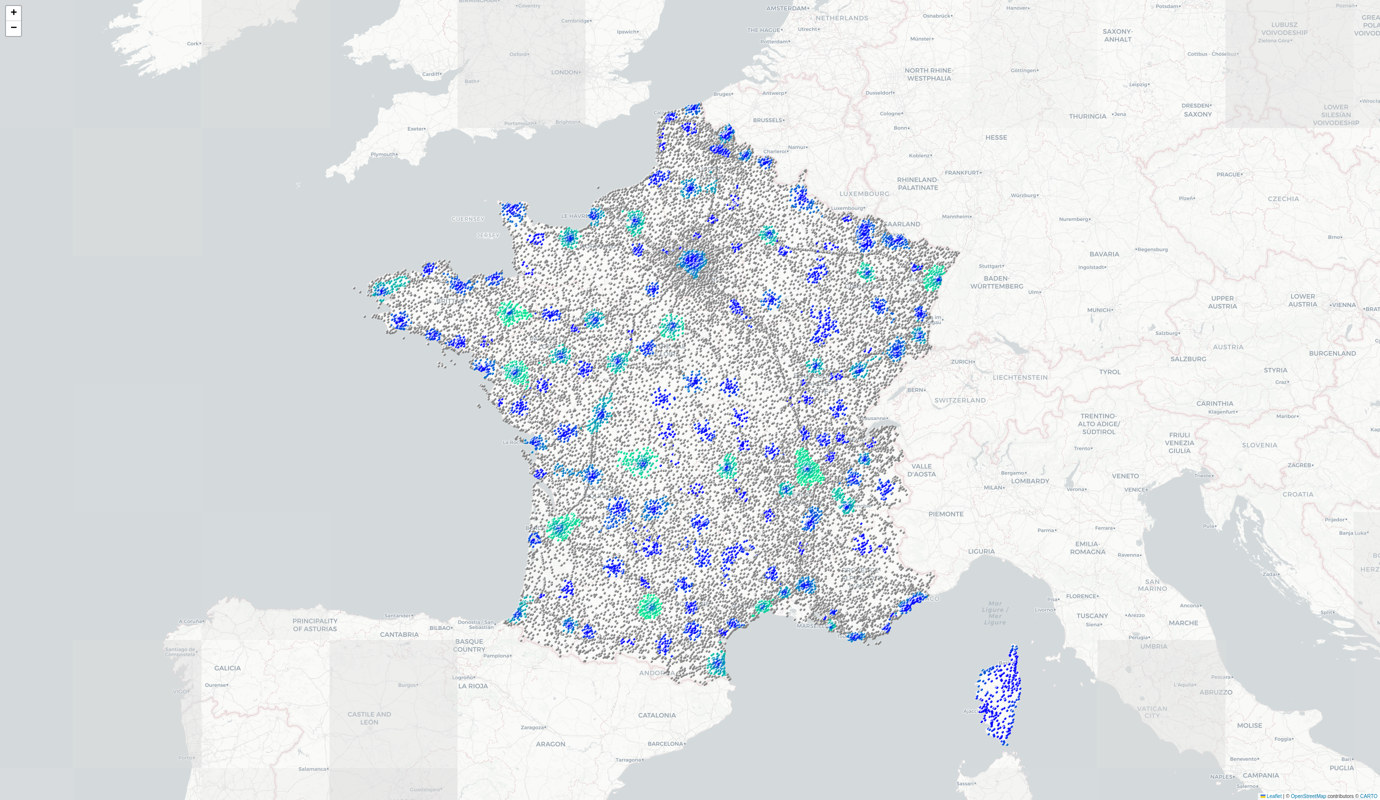
\includegraphics[width=0.9\paperheight]{images/villes_HDBSCAN.png}
        \caption{\label{fig:HDBSCAN}Application d'HDBScan \texttt{min\_cluster\_size=5}, \texttt{min\_samples=40}}
    \end{figure}
\end{frame}





% \smallframetitle

\section{Semaine du 27/05/24 au 31/05/24}
\insertsectionframe

\subsection{Comparaison des méthodes de détection des villes}
\insertsubsectionframe

\begin{frame}{HDBScan vs DBScan}
    \begin{columns}
        \begin{column}{0.5\textwidth}
            \begin{figure}
                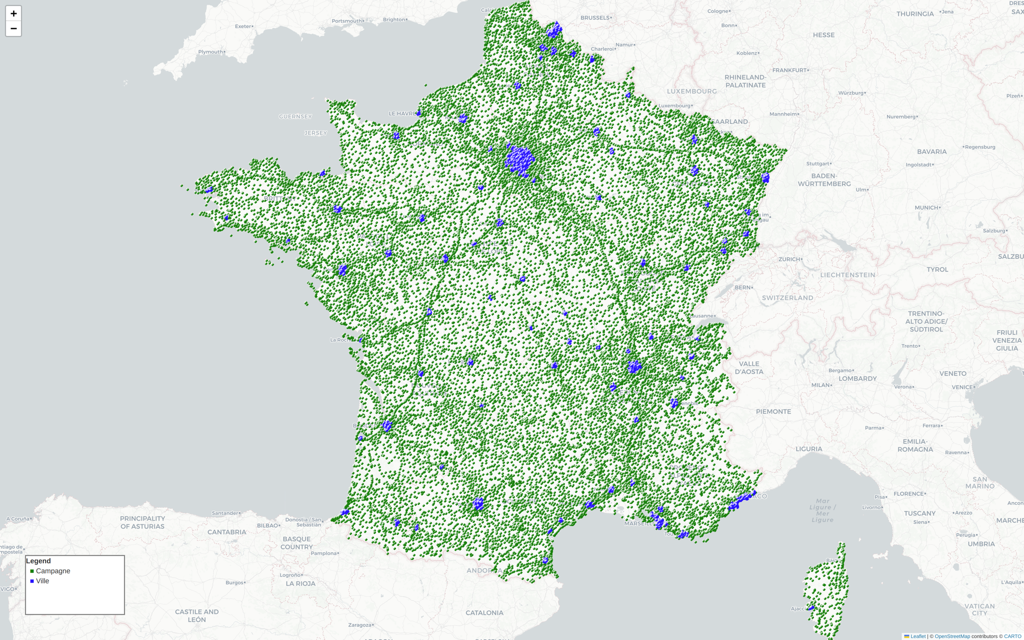
\includegraphics[width=0.4\paperwidth]{images/France-Villes-Orange_0.03_15.png}
                \caption{\label{fig:fr-vi-or-0.03-15-bis}Les villes détectées en France avec DBScan pour l'opérateur Orange avec $\epsilon=0.03$ et $n_{min}=15$}
            \end{figure}
        \end{column}
        \begin{column}{0.5\textwidth}
            \begin{figure}
                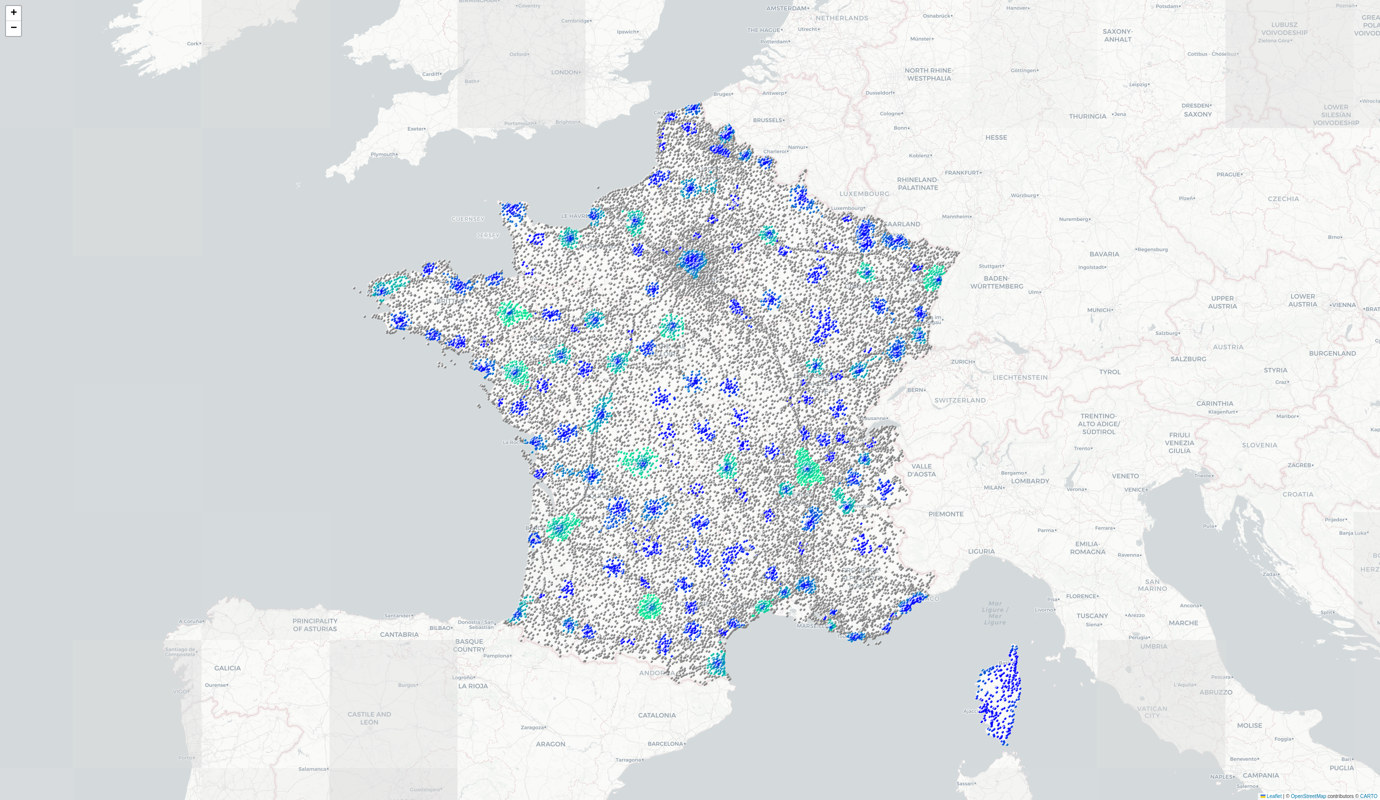
\includegraphics[width=0.4\paperwidth]{images/villes_HDBSCAN.png}
                \caption{\label{fig:HDBSCAN-bis}Les villes détectées en France avec HDBScan pour l'opérateur Orange avec \texttt{min\_cluster\_size=5}, \texttt{min\_samples=40}}
            \end{figure}
        \end{column}
    \end{columns}
\end{frame}

\subsection{Amélioration des critères de sélection}
\insertsubsectionframe

\begin{frame}{Prise en compte de la probabilité d'être dans une ville}
    \begin{block}{Concept}
        Chaque station possède une probabilité d'être dans une ville.
        On va donc utiliser ce paramètre afin de moduler l'angle et la distance minimale entre 2 stations.
    \end{block}

    \begin{block}{Choix d'implantation}
        Pour l'instant, on a séparé les stations en 4 catégories, en fonction de la probabilité d'être une ville:
        \begin{itemize}
            \item $p=1$ : \texttt{distance\_max = 1} et \texttt{min\_angle = 45};
            \item $p=0$ : \texttt{distance\_max = 15} et \texttt{min\_angle = 15};
            \item $p\in\left]1 ; 0,6\right[$ : \texttt{distance\_max = 5} et \texttt{min\_angle = 30};
            \item $p\in\left[0,6 ; 0\right[$ : \texttt{distance\_max = 10} et \texttt{min\_angle = 20}.
        \end{itemize}
    \end{block}
    
    \begin{alertblock}{Pistes de travail}
        Il va maintenant falloir effectuer des expérimentations pour trouver les bons paramètres et peut-être essayer de savoir quel paramètre est le plus pertinent.
    \end{alertblock}
\end{frame}

\begin{frame}{Améliorations des cadrants}
    \begin{block}{KNN}
        Dans un premier temps, nous avons décidé de pouvoir chosir le nombre de voisins par cadran que nous souhaitons conserver.
        Cette amélioration ne semble pas très concluante car la méthode devient trop permissive pour $k \geq 2$ (4190 / 4337 voisins conservés).
    \end{block}
    \begin{block}{Optimisation du positionnement des cadrans}
        La position de cadran est choisie en testant un angle $\alpha$ qui est décalage angulaire pour positionner le cadran.
        L'angle $\alpha$ choisi est la valeur entre 0 et 60 degrés qui maximise la distance entre les points et la limite de cadran la plus proche.
    \end{block}
\end{frame}

\begin{frame}{Illustration de l'optimisation du positionnement du cadran}
    \begin{columns}
        \begin{column}{0.5\textwidth}
            \begin{figure}
                \includegraphics[height=0.5\paperheight]{images/quadrants_sans_décalage.png}
                \caption{\label{fig:quad_sans_decalage} Quadrants non optimisés}
            \end{figure}
        \end{column}
        \begin{column}{0.5\textwidth}
            \begin{figure}
                \includegraphics[height=0.5\paperheight]{images/quadrants_avec_décalage.png}
                \caption{\label{fig:quad_avec_decalage} Quadrants optimisés}
            \end{figure}
        \end{column}
    \end{columns}
\end{frame}


\smallframetitle

\section{Semaine du 03/06/24 au 06/06/24}
\insertsectionframe

\subsection{Comparaison des résultats de 2 détection de villes}
\insertsubsectionframe

\begin{frame}{Affichage}
    \begin{columns}
        \begin{column}{0.5\textwidth}
            \begin{block}{Affichage des différences}
                Afin de visualiser les différences, nous pouvons tracer les 2 classifications en même temps sur une carte en adoptant ce code couleur :
                \begin{itemize}
                    \item Rouge : station en ville dans les 2 classification;
                    \item Bleu : station en ville dans exactement 1 classification;
                    \item Vert : station en campagne dans les 2 classifications.
                \end{itemize}
            \end{block}
        \end{column}

        \begin{column}{0.5\textwidth}
            \begin{figure}
                \includegraphics[height=0.5\paperheight]{images/city_comparison.png}
                \caption{\label{fig:city-comparison}Comparaison des résultats de détection de villes : DBScan vs HDBScan}
            \end{figure}
        \end{column}
    \end{columns}
    
    
\end{frame}


\begin{frame}{Indicateurs}
    \begin{block}{Indicateurs de base}
        Nous avons dévéloppé quatre indicateurs de base afin de caractériser la similarité entre deux classifications :
        \begin{itemize}
            \item $a$ : Le pourcentage de station en ville dans les deux classifications;
            \item $b$ : Le pourcentage de station en ville dans la première classification et non la deuxième;
            \item $c$ : Le pourcentage de station en ville dans la deuxième classification et non la première;
            \item $d$ : Le pourcentage de station en campagne dans les deux classifications.
        \end{itemize}
    \end{block}
    \begin{block}{Résultats}
        Sur les classifications présentées dans la slide précédentes, voici les résultats obtenus : 
        \begin{itemize}
            \item $a = 0,688$;
            \item $b = 0,028$;
            \item $c = 0,051$;
            \item $d = 0,232$.
        \end{itemize}
    \end{block}
\end{frame}


\subsection{Nouvelle manière de détecter les villes}
\insertsubsectionframe

\begin{frame}{Changement de cap} 
    \begin{block}{Problèmes rencontrés avec DBScan et HDBScan}
        \begin{itemize}
            \item Méthodes complexes donc peu prévisibles;
            \item Résultats non-satisfaisants quand le méthode est appliquée à seulement une partie de la France.
            \item DBScan est trop binaire, HDBScan est à densité variable donc ne détecte pas toutes les villes de la même façon (problème avec Paris notamment)
            \item Les probabilités de HDBScan ne caractérisent pas exactement la probabilité d'être en ville mais plutôt la certitude avec laquelle on peut rattacher un point à son cluster.
        \end{itemize}
    \end{block}

    \begin{block}{Réflexion sur une méthode plus simple}
        Nous souhaitions savoir quelle station se trouvait en ville, car on sait qu'en ville, les stations sont plus proches les unes des autres, donc les rayons de couverture plus courts.
        Cependant, il n'est pas nécessaire de detecter les villes pour cela, nous pouvons simplement regarder la distance moyenne aux $k$ plus proches voisins.
    \end{block}

\end{frame}

\begin{frame}{Méthodologie}
    \begin{block}{Nouvelle méthode}
        Au lieu d'utiliser une méthode de clustering, nous allons utiliser quelque chose de plus simple.
        On classifie chaque station selon la distance moyenne aux $3$ plus proches voisins. %2 c'est pas assez pour avoir quelquechose de palapable, 4 augmente trop la distance.
        Soit $d$ cette distance, on regroupe les stations de la manière suivante:
        \begin{itemize}
            \item $d\in\left]0, 1\right]$ : centre ville dense;
            \item $d\in\left]1, 2\right]$ : couronne périhurbaine;
            \item $d\in\left]2, 5\right]$ : campagne;
            \item $d\in\left]5, 10\right]$ : campagne profonde;
            \item $d\in\left]10, \infty\right[$ : trou paumé ou valeur aberrante.
        \end{itemize}
    \end{block}
\end{frame}

\begin{frame}{Méthodologie : choix techniques}
    \begin{block}{Calcul des plus proches voisins}
        Nous utilisons la bibliothèque \emph{sklearn.neighbors.NearestNeighbors}\footnotemark.
    \end{block}

    \begin{block}{Choix du nombre de voisins}
        Après plusieurs expérimentations, nous avons choisi de conserver $3$ voisins dans notre calcul.
        En effet, un chiffre inférieur à $2$ serait aberrant car ce ne serait pas une vraie moyenne (ici on cherche plus une mesure de la densité de stations).
        De plus, un chiffre supérieur à $4$ prendrait en compte des stations trop éloignées, ce qui serait aberrant.
    \end{block}
    
    \begin{block}{Métrique}
        Nous avons décidé de partir de la projection de Lambert 93 (qui est déjà présente dans nos données) pour calculer cette distance.
        L'avantage est le gain de temps (environ 30 fois plus rapide), sans perte de performance, par rapport à la conversion en $\unit{km}$ depuis les coordonnées Longitude, Latitude.
    \end{block}

    \footnotetext{\url{https://scikit-learn.org/stable/modules/generated/sklearn.neighbors.NearestNeighbors.html}}
\end{frame}

\begin{frame}{Mise à jour des critères}
    \begin{columns}
        \begin{column}{0.4\paperwidth}
            \begin{block}{Angle}
                Voici les différents paliers que nous appliquons :
                \begin{itemize}
                    \item $d\in\left]0, 1\right]$ : $\text{angle\_min}=40^\circ$;
                    \item $d\in\left]1, 2\right]$ : $\text{angle\_min}=30^\circ$;
                    \item $d\in\left]2, 5\right]$ : $\text{angle\_min}=25^\circ$;
                    \item $d\in\left]5, 10\right]$ : $\text{angle\_min}=15^\circ$;
                    \item $d\in\left]10, \infty\right[$ : $\text{angle\_min}=10^\circ$.
                \end{itemize}
            \end{block}
        \end{column}
        \begin{column}{0.4\paperwidth}
            \begin{block}{Distance}
                Voici les différents paliers que nous appliquons :
                \begin{itemize}
                    \item $d\in\left]0, 1\right]$ : $\text{distance\_max}=\unit[2]{km}$;
                    \item $d\in\left]1, 2\right]$ : $\text{distance\_max}=\unit[5]{km}$;
                    \item $d\in\left]2, 5\right]$ : $\text{distance\_max}=\unit[10]{km}$;
                    \item $d\in\left]5, 10\right]$ : $\text{distance\_max}=\unit[15]{km}$;
                    \item $d\in\left]10, \infty\right[$ : $\text{distance\_max}=\unit[15]{km}$.
                \end{itemize}
            \end{block}
        \end{column}
    \end{columns}
\end{frame}

\selectlanguage{english}

\selectlanguage{english}

\smallframetitle

\section{From 10/06/24 to 14/06/24}
\insertsectionframe

\subsection{Modification of criteria}
\insertsubsectionframe

\begin{frame}{New criteria and city classification}
    After some reflexions, we have agreed to change the way we classify the city-ness of each base station :
    \begin{block}{New city-ness classification}
        \begin{columns}
            \begin{column}{0.4\paperwidth}
                \begin{itemize}
                    \item $d\in\left]0, 1\right]$ : city center;
                    \item $d\in\left]1, 2\right]$ : urban area;
                \end{itemize}
            \end{column}
            \begin{column}{0.4\paperwidth}
                \begin{itemize}
                    \item $d\in\left]2, 4\right]$ : extra-urban area;
                    \item $d\in\left]4, \infty\right[$ : courntryside.
                \end{itemize}
            \end{column}
        \end{columns}
    \end{block}
    \begin{columns}
        \begin{column}{0.4\paperwidth}
            \begin{block}{Angle}
                \begin{itemize}
                    \item $d\in\left]0, 1\right]$ : $\text{angle\_min}=40^\circ$;
                    \item $d\in\left]1, 2\right]$ : $\text{angle\_min}=30^\circ$;
                    \item $d\in\left]2, 4\right]$ : $\text{angle\_min}=25^\circ$;
                    \item $d\in\left]4, \infty\right[$ : $\text{angle\_min}=15^\circ$.
                \end{itemize}
            \end{block}
        \end{column}
        \begin{column}{0.4\paperwidth}
            \begin{block}{Distance}
                \begin{itemize}
                    \item $d\in\left]0, 1\right]$ : $\text{distance\_max}=\unit[2]{km}$;
                    \item $d\in\left]1, 2\right]$ : $\text{distance\_max}=\unit[5]{km}$;
                    \item $d\in\left]2, 4\right]$ : $\text{distance\_max}=\unit[10]{km}$;
                    \item $d\in\left]4, \infty\right[$ : $\text{distance\_max}=\unit[15]{km}$.
                \end{itemize}
            \end{block}
        \end{column}
    \end{columns}
\end{frame}


\subsection{City detection results comparison}
\insertsubsectionframe

\begin{frame}{Reminder : the brute results}
    \begin{figure}
        \includegraphics[height=0.6\paperheight]{images/city-detection.png}
        \caption{\label{fig:city-detection}City detection by respectively DBScan, HDBScan and 3-NN methods}
    \end{figure}
\end{frame}

\begin{frame}{Graphical methods comparison}
    \begin{figure}
        \includegraphics[height=0.6\paperheight]{images/city-detection-comparison.png}
        \caption{\label{fig:city-detection-comparison}DBScan vs HDBScan / HDBScan vs 3-NN / DBScan vs 3-NN}
    \end{figure}
\end{frame}

\begin{frame}{Numerical methods comparison}
    \begin{columns}
        \begin{column}{0.22\paperwidth}
            \begin{block}{DBScan vs HDBScan}
                \begin{itemize}
                    \item $a=0.688$
                    \item $b=0.028$
                    \item $c=0.052$
                    \item $d=0.232$
                \end{itemize}
            \end{block}
        \end{column}
        \begin{column}{0.22\paperwidth}
            \begin{block}{HDBScan vs 3-NN}
                \begin{itemize}
                    \item $a=0.626$
                    \item $b=0.114$
                    \item $c=0.010$
                    \item $d=0.250$
                \end{itemize}
            \end{block}
        \end{column}
        \begin{column}{0.22\paperwidth}
            \begin{block}{DBScan vs 3-NN}
                \begin{itemize}
                    \item $a=0.630$
                    \item $b=0.086$
                    \item $c=0.007$
                    \item $d=0.277$
                \end{itemize}
            \end{block}
        \end{column}
    \end{columns}
\end{frame}

\subsection{Improvement of City detection}
\insertsubsectionframe

\begin{frame}{Reminder : functionnement of base 3-NN}
    \begin{figure}
        \includegraphics[height=0.6\paperheight]{images/illustration_3-NN.png}
        \caption{\label{fig:illus-3-NN}How 3-NN method works}
    \end{figure}
\end{frame}

\smallframetitle

\section{From 17/06/24 to 21/06/24}
\insertsectionframe

\subsection{Road detection method - in progress}
\insertsubsectionframe

\begin{frame}{Methodology}
    We have seen that one classification with either DBScan or HDBScan isn't enough. So, why not combining them.
    \begin{block}{The base idea}
        We will combine the clusters of DBScan, HDBScan and OPTICS (another density base clustering method) to try to find roads.
    \end{block}

    \begin{block}{One problem}
        We are now able to detect road/railways but the problem is that there is still little clusters that are useless.
    \end{block}
\end{frame}

\begin{frame}{New method illustration (1/2)}
    \begin{columns}
        \begin{column}{0.4\paperwidth}
            \begin{figure}
                \boxed{\includegraphics[width=0.4\paperwidth]{images/road_detection/clust1.png}}
                \caption{One clustering method}
            \end{figure}
        \end{column}
        \begin{column}{0.4\paperwidth}
            \begin{figure}
                \boxed{\includegraphics[width=0.4\paperwidth]{images/road_detection/clust2.png}}
                \caption{Another clustering method}
            \end{figure}
        \end{column}
    \end{columns}
\end{frame}

\begin{frame}{New method illustration (2/2)}
    \begin{columns}
        \begin{column}{0.4\paperwidth}
            \begin{figure}
                \boxed{\includegraphics[width=0.4\paperwidth]{images/road_detection/merge_clust.png}}
                \caption{Merge of the clusters}
            \end{figure}
        \end{column}
        \begin{column}{0.4\paperwidth}
            \begin{figure}
                \boxed{\includegraphics[width=0.4\paperwidth]{images/road_detection/elimination.png}}
                \caption{Elimination of noise}
            \end{figure}
        \end{column}
    \end{columns}
\end{frame}

\begin{frame}{DBScan clustering}
    \begin{figure}
        \includegraphics[height=0.6\paperheight]{images/cartes/road_detection/dbs.png}
        \caption{DBScan clustering}
    \end{figure}
\end{frame}

\begin{frame}{HDBScan clustering}
    \begin{figure}
        \includegraphics[height=0.6\paperheight]{images/cartes/road_detection/hdb.png}
        \caption{HDBScan clustering}
    \end{figure}
\end{frame}

\begin{frame}{OPTICS clustering}
    \begin{figure}
        \includegraphics[height=0.6\paperheight]{images/cartes/road_detection/opt.png}
        \caption{OPTICS clustering}
    \end{figure}
\end{frame}

\begin{frame}{Result}
    \begin{figure}
        \includegraphics[height=0.6\paperheight]{images/cartes/road_detection/res.png}
        \caption{Road detection}
    \end{figure}
\end{frame}

\subsection{More details and problems}
\insertsubsectionframe

\begin{frame}{Detailed clusters detected}
    \begin{figure}
        \includegraphics[height=0.6\paperheight]{images/clusters_road_detection.html.png}
        \caption{Detailed clusters detected in coutryside by each method}
    \end{figure}
\end{frame}

\begin{frame}{Problems and ideas}
    \begin{block}{Problems}
        \begin{itemize}
            \item A lot of little citys detected : not only roads ;
            \item The areas around big citys are a mess ;
            \item HDBScan has only one cluster.
        \end{itemize}
    \end{block}

    \begin{block}{Ideas}
        \begin{itemize}
            \item Refine the parameters of each method ;
            \item Use linear regressions to detect parts of roads and maybe help propagate them.
        \end{itemize}
    \end{block}
\end{frame}

\subsection{Altair AI Studio Software Review}
\insertsubsectionframe

\begin{frame}{Altair AI Studio Software Review}
    Objective is to evaluate Altair AI Studio for their potential to enhance our research on classifying the terrain of mobile base stations.
    Available at: \url{https://altair.com/altair-ai-studio}
    \begin{block}{Altair AI Studio}
        This is a platform designed for data analysis and machine learning model building. Possible benefits for us:
        \begin{itemize}
            \item Supports clustering and classification algorithms.
            \item Support for various machine learning algorithms.
            \item Enables effective result visualization (graphs) for enhanced analysis.
        \end{itemize}
    \end{block}
    \begin{columns}
        \begin{column}{0.4\paperwidth}
            \begin{block}{Key Features:}
                \begin{itemize}
                    \item Integration with various data sources.
                    \item Interactive model creation and testing.
                    \item Support for various machine learning algorithms.
                \end{itemize}
            \end{block}
        \end{column}
        \begin{column}{0.4\paperwidth}
            \begin{block}{Users:}
                \begin{itemize}
                    \item Data researchers
                    \item Analysts
                    \item Machine learning developers
                \end{itemize}
            \end{block}
        \end{column}
    \end{columns}
\end{frame}

\begin{frame}{Example of Usage in Altair AI Studio}
    \begin{figure}
        \includegraphics[height=0.6\paperheight]{images/Altair/Altair_proc_exmpl.png}
        \caption{How Altair AI Software works}
    \end{figure}
\end{frame}


\subsection{New Possible Approach for Terrain Classification}
\insertsubsectionframe

\begin{frame}{More accurate verification of the classification of base station locations}
We want to validate and enhance the previous classification of base station locations by leveraging a new geographic dataset. 
We found and will try to use a comprehensive dataset from \url{data.enseignementsup-recherche.gouv.fr}, which includes precise geographic data points across France with pre-defined zone classifications.
\begin{block}{Methodology for Base Station Classification}
    Previously, we worked with a dataset containing locations of all base stations. Now, we utilize an additional dataset with geographic points across France, each classified into zones (urban, suburban, rural). By comparing base station coordinates with these geographic points, we determine the zone of each base station. The closest geographic point's classification is assigned to the base station, providing a more accurate terrain classification.
\end{block}
    \begin{block}{Benefits:}
        \begin{itemize}
            \item Cross-reference base station coordinates with geographic data points to accurately assign zone classifications.
            \item Provides an additional layer of verification and accuracy for our classification methods.
        \end{itemize}
    \end{block}
\end{frame}



\begin{frame}{Classification of points in the new dataset}
    \begin{figure}
        \includegraphics[height=0.6\paperheight]{images/Geo_approach/New_dataset_points_ill.png}
        \caption{Classification of points from the new dataset}
    \end{figure}
\end{frame}
\begin{frame}{Classification of points in the new dataset}
    \begin{block}{Geographic identifiers:}
        \begin{itemize}
        \item UU (Urban Units): Areas classified as urban units.
        \item CR (Rural Communes): Areas classified as rural communes.
        \item AU (Urban Areas): Larger urban areas or agglomerations.
        \end{itemize}
    \end{block}
    \begin{block}{Methodology and Challenges}
            This method helps classify base station locations by comparing them with geographic data points. However, we need to preprocess the dataset carefully and address the issue of having a limited number of points. To ensure high accuracy, we might need to augment the data or combine it with other datasets for better coverage and precision
    \end{block}
\end{frame}

\subsection{Another new database}
\insertsubsectionframe

\begin{frame}{New possibilities on city/countryside classification}
    \begin{columns}
        \begin{column}{0.4\paperwidth}
            \begin{figure}
                \boxed{\includegraphics[width=0.4\paperwidth]{images/cartes/new_databases/new_database.png}}
                \caption{Database we presented last week}
            \end{figure}
        \end{column}
        \begin{column}{0.4\paperwidth}
            \begin{figure}
                \boxed{\includegraphics[width=0.4\paperwidth]{images/cartes/new_databases/new-new_database.png}}
                \caption{A new database (cities with more than $5000$ inhabitants)}
            \end{figure}
        \end{column}
    \end{columns}
\end{frame}

\begin{frame}{What's this?}
    We found a new database on the population of each french commune in 2021\footnote{\url{https://www.insee.fr/fr/statistiques/7739582}}.
    \begin{block}{INSEE?}
        It is the National Institute of Statistics and Economics Studies. It collects, analyses and disseminates information on the French economy and society.
    \end{block}

    \begin{block}{Why this one?}
        Firstly, this database is really recent (updated on 26/01/2024). Then, the other database we introduced was to permisive in the definition of what is a city (a commune with more than $2000$ inhabitants).
        So we wanted something more flexible.
    \end{block}
\end{frame}

\subsection{Back to road detection}
\insertsubsectionframe

\begin{frame}{HDBScan parameters adaptation}
    \begin{figure}
        \boxed{\includegraphics[height=0.6\paperheight]{images/hdbscan_roads_crude.png}}
        \caption{Result of HDBScan with new parameters on countryside to detect roads}
    \end{figure}
\end{frame}

\begin{frame}{A bit of math theory (1/2)}
    \begin{block}{Multiple linear regression}
        Let a dataset be composed of $m$ vectors$\ensuremath{\left(x^{i}\right)_{i\in\left\{ 1\dots m\right\} }}$
        of $\mathbb{R}^{n}$, ie $\forall i\in\{1,\dots ,m\}$, $x^{i}=(x_{1}^{i},\dots,x_{n}^{i})$. 

        Let $\left(y^{i}\right)_{i\in\left\{ 1\dots m\right\}}$
        be $m$ associated values in $\mathbb{R}$.

        Then, we can find a linear function $f:\mathbb{R}^{n}\rightarrow\mathbb{R}$
        (ie $f(x_{1},\dots,x_{n})=c_{1}x_{1}+\dots+c_{n}x_{n}$) that minimises
        the error : $\Vert\sum_{i=1}^{m}(f(x^{i})-y^{i})\Vert$

        $f$ is called a multiple linear regression associated to $\left(x^{i}\right)_{i\in\left\{ 1\dots m\right\}}$
        and $\left(y^{i}\right)_{i\in\left\{ 1\dots m\right\}}$.
    \end{block}
    \begin{figure}
        \boxed{\includegraphics[height=0.3\paperheight]{images/multiple_linear_regression.png}}
        \caption{Example of multiple linear regression with $n=2$}
    \end{figure}
\end{frame}

\begin{frame}{A bit of math theory (2/2)}
    \begin{block}{Polynomial regression}
        Let a dataset be composed of $m$ values $\left(x^{i}\right)_{i\in\left\{ 1\dots m\right\} }$ of $\mathbb{R}$. 

        Let $\ensuremath{\left(y^{i}\right)_{i\in\left\{ 1\dots m\right\}}}$ be $m$ associated values in $\mathbb{R}$.

        We can transform the data in $m$ vectors$\left(x^{i}\right)_{i\in\left\{ 1\dots m\right\}}$
        of $\mathbb{R}^{n+1}$ defined by $(x_{0}^{i},x_{1}^{i},x_{2}^{i},\dots,x_{n}^{i})=(1,x^{i},(x^{i})^{2},\dots,(x^{i})^{n})$, 
        and then apply the multiple linear regression seen earlier on this transormed data.
        
        We therefore obtain a function 
        \[
            f:\begin{cases}
            \mathbb{R}\rightarrow\mathbb{R}\\
            x\mapsto c_{1}+c_{2}x+\dots+c_{n}x^{n}
            \end{cases}
        \]
        
        That is a degree $n$ polynome that approximates the relation between $x$ and $y$.
    \end{block}

    \begin{block}{Quantify the quality of the approximation}
        As for the simple linear regression, we obtain a $R$ coefficient between $0$ and $1$ that indicates if the approximation is close to the original data 
        (i.e. if the polynome we find at the end is close to the real appearance of the data).
    \end{block}
\end{frame}

\begin{frame}{Application of the method on each cluster of HDBScan}
    \begin{figure}
        \boxed{\includegraphics[height=0.6\paperheight]{images/hdbscan_roads.png}}
        \caption{Approximation of each cluster by a degree 20 polynome}
    \end{figure}
\end{frame}

\begin{frame}{Filtration of the cluster by keeping the ones that have a $R$ coefficient above a value}
    \begin{figure}
        \boxed{\includegraphics[height=0.6\paperheight]{images/hdbscan_roads_filtered.png}}
        \caption{Approximation of each cluster by a degree 20 polynome, keeping only the ones with a $R$ coefficient above $0.2$}
    \end{figure}
\end{frame}

\smallframetitle

\section{From 24/06/24 to 28/06/24}
\insertsectionframe

\subsection{New ideas on neighbours detection}
\insertsubsectionframe

\begin{frame}{Neighbours detection without Delaunay}
    Just to see, we asked ourselves: why not trying to find neighbours without the Delaunay triangulation? Here is our methodology:

    \begin{block}{Creating the potential-neighbours-graph}
        The base idea was to firstly create a graph. But how?

        We will use the maximum distance to connect base stations according to the distance criteria,
        i.e. we connect a base station to surrounding stations that are in the radius of $max\_distance$.
    \end{block}

    And then we apply the angle and quadrant criteria like before.
    
    \begin{block}{Is it worth it?}
        It gives results that are more or less the same than before, but there are some imperfections.
        So, we could say that this is interesting but not really useful.
    \end{block}
\end{frame}

\subsection{Here come\dots}
\insertsubsectionframe

\begin{frame}{\dots a newer database!}
    Because the other databases we found earlier were not really convincing (in fact they are just useful to compare results).
    We therefore did some other research and found some interesting things!

    \begin{block}{ANFR}
        The National FRequency Agency, a public administrative body, was set up by the Telecommunications Regulation Act of 26 July 1996
        to plan, manage and monitor the use of public radio frequencies in France.
    \end{block}

    \begin{block}{The database itself}
        In this database\footnotemark, you have a map of all base stations in France. The interest of this database is that we can have all the frequencies used in one site and the orientation of the antennas.

        However, the problem is that we cannot download this database.
    \end{block}

    So, let's find a downloadable database.

    \footnotetext{\url{https://www.cartoradio.fr/\#/cartographie/stations}}
\end{frame}

\begin{frame}{\dots a newer database! - bis}
    This is another database from ANFR. This time we have the frequencies used in the databases.
    
    We linked those results in the first database by only keeping the highest frequency per base station.
\end{frame}

\subsection{Analysis of Frequency Data for Mobile Operators in France}
\insertsubsectionframe

\begin{frame}{France spectrum - mobile network frequency plan}
    We have detailed data on the frequency spectrums used by mobile operators in France. This data allows us to understand the specific frequencies at which each base station operates.
    \begin{block}{Frequency Bands:}
        \begin{itemize}
            \item The primary frequency bands used for 4G LTE in France include 700 MHz, 800 MHz, 1800 MHz, 2100 MHz, and 2600 MHz.
            Each frequency band has its own characteristics in terms of range, penetration, and data capacity.
        \end{itemize}
    \end{block}
    \begin{figure}
        \includegraphics[height=0.4\paperheight]{images/Altair/Or_spectrum.png}
        \caption{Orange Mobile network frequency plan}
    \end{figure}
\end{frame}

\begin{frame}{Analysis of Frequency Data for Orange}
    \begin{figure}
        \includegraphics[height=0.6\paperheight]{images/Altair/Or_4g_freq_compar.png}
        \caption{Count of antennas operating at each frequency band}
    \end{figure}
\end{frame}

\begin{frame}{Analysis of Frequency Data}
    \begin{block}{Characteristics of each band}
        \begin{itemize}
            \item 700 MHz and 800 MHz: Long-range, good building penetration.
            \item 1800 MHz and 2100 MHz: Balanced range and capacity.
            \item 2600 MHz: Short-range, high capacity.
        \end{itemize}
    \end{block}

    \begin{block}{Methodology for Coverage Calculation}
        To estimate the coverage zones of mobile base stations using only frequency data, we can implement the following approach. 
        
        We can apply standard radio propagation models such as the Hata Model for urban areas and the Cost-231 for suburban and rural areas.
        These models allow us to estimate coverage zones based on the operating frequency of each base station. Despite lacking specific data on transmission power, antenna gain, path loss, and receiver sensitivity, these propagation models provide a generalized prediction of signal coverage areas by leveraging established empirical data and frequency characteristics.
        This methodology can enable us to approximate the coverage zones for each frequency band.
    \end{block}
\end{frame}

\begin{frame}
    \frametitle{LTE RF Link Budgeting Model}
    \begin{itemize}
        \item The link budget calculations are needed for the calculation of cellular coverage parameters.
        \item A link budget takes into consideration all the losses and gains involved in equipment (e.g., BTS), end-terminals (e.g., mobile devices), and communication medium (e.g., free space).
        \item The results obtained indicate the maximum allowable propagation loss (MAPL). The formulae used in the link budget calculations are expressed below:
    \end{itemize}
    \begin{block}{Link budget calculations}
        \begin{align}
            EIRP_{Tx} &= P_{Tx} + G_{Tx} - L_b \\
            EIRP_{Tx} &= NB_{noise} + Th_{noise} + SINR \\
            MAPL &= EIRP_{Tx} + R_{SENS} - IM - L_{cable} + G_{Rx} - M + G_{soft}
        \end{align}
    \end{block}
    \textbf{Note:} We do not have exact data for our base stations, but we can make reasonable assumptions based on industry standards.
    \end{frame}

\begin{frame}{Reference Research Findings}
    We have referenced research that provides input parameters for radio propagation models and cell-range calculation results.
    \begin{block}{Input parameters for radio propagation model}
        \begin{itemize}
            \item Carrier Frequencys (MHz): 700, 800, 1800, and 2100 MHz.
            \item Base Station Height (hb): Typically around 30 meters.
            \item Mobile Station Height (hm): Generally around 1.5 meters.
        \end{itemize}
    \end{block}
    \begin{figure}
        \includegraphics[height=0.35\paperheight]{images/Altair/cell_range_calc_res.png}
        \caption{Cell-range calculation results}
    \end{figure}
\end{frame}

\begin{frame}{Frequency Reuse Mode Challenges}
    \begin{columns}
        \begin{column}{0.55\textwidth}
            \begin{block}{Challenges with Unknown Frequency Reuse Mode}
                    \begin{itemize}
                        \item Each cell in a mobile network can be divided into sectors, each served by a different frequency.
                        \item The reuse of frequencies in different cells is essential to maximize the efficient use of the available spectrum.
                        \item Frequency reuse mode determines how frequencies are allocated across cells and sectors to minimize interference.
                        \item We lack detailed information on the specific frequency reuse mode utilized for each sector of our base stations.
                        \item Assumptions about uniform frequency reuse may not reflect the actual, varied configurations used in practice.
                    \end{itemize}
            \end{block}
        \end{column}
        \begin{column}{0.6\textwidth}
            \begin{figure}
                \includegraphics[height=0.4\paperheight]{images/Altair/Sectorization.png}
                \caption{Sectorization}
            \end{figure}
        \end{column}
    \end{columns}
\end{frame}

\smallframetitle

\section{From 01/07/24 to 05/07/24}
\insertsectionframe

\subsection{New road detection method}
\insertsubsectionframe

\begin{frame}{Building city connection graph (1/4)}
    \begin{columns}
        \begin{column}{0.4\textwidth}
            \begin{block}{City detection}
                A clustering method (here DBScan) is used only on the base station detected as a city center by the 3NN method.
                Thus, these base stations are now separated in different cities.
            \end{block}
        \end{column}
        \begin{column}{0.6\textwidth}
            \begin{figure}
                \includegraphics[width=0.5\paperwidth]{images/road_detection/city_clustering.png}
                \caption{city clustering}
            \end{figure}
        \end{column}
    \end{columns}        
\end{frame}

\begin{frame}{Building city connection graph (2/4)}
    \begin{columns}
        \begin{column}{0.4\textwidth}
            \begin{block}{Center computation}
                The center of each cluster is computed.
            \end{block}

            \begin{block}{city separation according to size}
                The cities that contain more than a certain number of stations are separated from the ones that contain less.
            \end{block}
        \end{column}
        \begin{column}{0.6\textwidth}
            \begin{figure}
                \includegraphics[width=0.5\paperwidth]{images/road_detection/city_clustering_with_centers.png}
                \caption{cities centers and size classification}
            \end{figure}
        \end{column}
    \end{columns}        
\end{frame}

\begin{frame}{Building city connection graph (3/4)}
    \begin{columns}
        \begin{column}{0.4\textwidth}
            \begin{block}{Delaunay triangulation}
                The Delaunay traingulation is then applied to the big cities to create a graph.
            \end{block}
        \end{column}
        \begin{column}{0.6\textwidth}
            \begin{figure}
                \includegraphics[height=0.3\paperheight]{images/road_detection/delaunay_big_cities_unfiltered.png}
                \caption{Big cities connection graph unfiltered}
            \end{figure}
        \end{column}
    \end{columns}        
\end{frame}

\begin{frame}{Building city connection graph (4/4)}
    \begin{block}{Graph filtration}
        The angle and distance criteria are then applied to filter the connections between the cities.
    \end{block}
    \begin{columns}
        \begin{column}{0.3\textwidth}
            \begin{figure}
                \includegraphics[width=0.2\paperwidth]{images/road_detection/delaunay_big_cities_unfiltered.png}
                \caption{Unfiltered}
            \end{figure}
        \end{column}
        \begin{column}{0.3\textwidth}
            \begin{figure}
                \includegraphics[width=0.2\paperwidth]{images/road_detection/delaunay_big_cities_distance_filtered.png}
                \caption{Distance filtered}
            \end{figure}
        \end{column}
        \begin{column}{0.3\textwidth}
            \begin{figure}
                \includegraphics[width=0.2\paperwidth]{images/road_detection/delaunay_big_cities_distance_angle_filtered.png}
                \caption{Distance and angle filtered}
            \end{figure}
        \end{column}
    \end{columns}        
\end{frame}

\end{document}
